\documentclass[ba]{imsart}
%
\pubyear{0000}
\volume{00}
\issue{0}
\doi{0000}
%\arxiv{}
\firstpage{1}
\lastpage{1}

\usepackage{amsthm}
\usepackage{amsmath}
\usepackage{natbib}
\usepackage[colorlinks,citecolor=blue,urlcolor=blue,filecolor=blue,backref=page]{hyperref}
\usepackage{graphicx}
\newtheorem{lemma}{Lemma}
\usepackage{booktabs}       % professional-quality tables
\usepackage{algorithm}      % algorithm environment
\usepackage{algpseudocode}

\startlocaldefs
\setbeamertemplate{navigation symbols}{}
\setbeamertemplate{footline}[page number]
\endlocaldefs

\begin{document}

%% *** Frontmatter *** 

\begin{frontmatter}
\title{Efficient and Scalable Bipartite Matching with Fast Beta Linkage  (fabl)}
%\title{A Sample Document\thanksref{T1}}
%\thankstext{T1}{<thanks text>}
\runtitle{Efficient and Scalable Bipartite Matching with Fast Beta Linkage  (fabl)}

\begin{aug}
\author{\fnms{Brian} \snm{Kundinger}\thanksref{addr1}\ead[label=e1]{brian.kundinger@duke.edu}},
\author{\fnms{Jerome} \snm{Reiter}\thanksref{addr1}\ead[label=e2]{jreiter@duke.edu}}
\and
\author{\fnms{Rebecca C.} \snm{Steorts}\thanksref{addr2}\ead[label=e3]{beka@stat.duke.edu}}

\runauthor{Kundinger et al.}

\address[addr1]{Department of Statistical Science,
  Duke University,
  P.O.\ Box 90251,
  Durham, NC 27708, USA
  \printead{e1}, % print email address of "e1"
  \printead*{e2}
}

\address[addr2]{Departments of Statistical Science and Computer Science,
  Duke University,
  P.O.\ Box 90251,
  Durham, NC 27708, USA
  \printead{e3}
}

%\thankstext{<id>}{<text>}
\end{aug}


\begin{abstract}
Recently, researchers have developed Bayesian versions of the Fellegi Sunter model for record linkage. These have the crucial advantage of quantifying uncertainty from imperfect linkages.  However, current implementations of Bayesian Fellegi Sunter models are computationally intensive, making them challenging to use on larger-scale record linkage tasks.  We propose and investigate a variation on Bayesian Fellegi Sunter models that we call fast beta linkage, or \texttt{fabl}.  Specifically, in \texttt{fabl} we propose independent prior distributions over the matching space, allowing us to use hashing techniques that reduce computational overhead. This also allows us to complete pairwise record comparisons over large datasets through parallel computing and reduce memory costs through a new technique called storage efficient indexing. Through simulations and two case studies, we show that \texttt{fabl} has markedly increased speed with minimal loss of accuracy.
\end{abstract}

%% ** Keywords **
\begin{keyword}%[class=MSC]
\kwd{bipartite record linkage}
\kwd{Bayesian methods}
\kwd{hashing techniques}
\kwd{parallel/distributed computing}
\kwd{Markov chain Monte Carlo}
\end{keyword}

\end{frontmatter}




%% ** Mainmatter **


\section{Introduction}
\label{sec:introduction}

In many data analysis tasks, analysts seek to identify duplicate records across two databases. This is an increasingly important task in ``data cleaning,'' and is used for inferential and predictive analyses in fields such as statistics, computer science, machine learning, political science, economics, precision medicine, official statistics, and others \citep{christen_2012, gutman2013bayesian, DalzellReiter18, tang2020}. In this article, we consider bipartite record linkage, which merges two databases together that contain duplications across but not within the respective databases. 

Many statistical record linkage methods are extensions of the seminal work of \cite{fellegi_theory_1969} and \cite{newcombe_automatic_1959}. Specifically, \cite{fellegi_theory_1969} created comparison vectors for each pair of records in the data and independently classified each pair as a match or a non-match using a likelihood ratio test. Recent work in the statistical literature has extended this approach for a wide variety of applications \citep{Winkler1990, fair2004generalized, wagner2014person, gill2003english, enamorado2019using, aleshinguendel2021multifile}. Additionally, some methods model records directly \citep{steorts_bayesian_2016, marchant_distributed_2019, betancourt2021prior}, but in this paper, we build on the contributions to the comparison vector approach. 

% Possible citation for bipartite matching. 
%\citep{fellegi_theory_1969, jaro1989, Winkler1988, belin_1995, larsen_2001, liseo_2011,  herzog2007data, gutman_bayesian_2013, sadinle_bayesian_2017}.

The independent pairwise matching assumption from \cite{fellegi_theory_1969} is popular mainly for its mathematical simplicity, but can be unreasonable in practice. In many situations, we know that there are no duplications within a database, meaning that each record should be linked with at most one other record. Thus, when the procedure results in many to one matches, some of these links must be false. Many extensions to \cite{fellegi_theory_1969} resolve these false matches as a post-processing step \citep{jaro1989}, but this model misspecification can still lead to poor results \citep{sadinle_bayesian_2017}.

Alternatively, one can embed one-to-one matching requirements into the model specification itself \citep{gutman2013bayesian, liseo_2011}, at an additional computational cost. \cite{Larsen05} employed a Metropolis-Hastings algorithm to only allow sampling matches that respected one-to-one assumptions, but such algorithms exhibit slow mixing due to the combinatorial nature of the constrained matching space. \cite{fortunato_2010} used simulated annealing to target the space of matches permitted under the one-to-one constraint, but the method is quite computationally intensive and, to our knowledge, has not been applied on databases with more than 100 records. \cite{sadinle_bayesian_2017} proposed the Beta Record Linkage model (\texttt{BRL}), using a prior over the space of bipartite matchings to strictly enforce one-to-one requirements throughout a Gibbs sampler. Additionally, he introduced a class of loss functions that allows for a flexible estimation of the linkage structure, such that the modeller can weight the relative importance of false positives and false negatives, and identify records pairings to be decided through clerical review. \texttt{BRL} was shown to work on larger tasks than previous one-to-one methods, but in our experience, it becomes slow when applied to files with more than a few thousand records. 

In this paper, we propose fast beta linkage (\texttt{fabl}), which extends the \texttt{BRL} model for increased efficiency and scalability. Following the suggestion in \cite{wortman2019}, we relax the one-to-one matching requirement of \texttt{BRL} and propose independent priors over the matching space, creating a ``many-to-one'' model for record linkage. This allows us to (1) employ hashing techniques that speed up calculations and reduce computational costs, (2) compute the pairwise record comparisons over large datasets via parallel computing, and (3) reduce memory costs through what we call storage efficient indexing. We demonstrate that even in cases where a bipartite matching is desired, \texttt{fabl} (with a simple post-processing procedure) provides accurate estimation of the linkage structure and other parameters, more information through which to asses model misspecification, and greatly enhanced speed. Open source software to use \texttt{fabl} in \texttt{R} is available through \href{https://github.com/briankundinger/parlrdev}{Github}.

In what follows, Section~\ref{sec:review-of_prior-work} reviews the work of \cite{fellegi_theory_1969} and \cite{sadinle_bayesian_2017}. Section~\ref{sec:fast-beta-linkage}, proposes the \texttt{fabl} model, derives the Gibbs sampler for posterior inference, and provides the loss function used to calculate the Bayes estimate for the bipartite matching. Section~\ref{sec:efficiency} introduces the hashing technique and storage efficient indexing used to increase the speed of calculatoins and the scale of linkage tasks amenable to \texttt{fabl}. Sections~\ref{sec:simulations} and \ref{sec:case-studies} demonstrate the speed and accuracy of \texttt{fabl} through simulation studies and case studies of homicides from the El Salvadoran Civil War and the National Long Term Care Study.

\section{Review of Prior Work}
\label{sec:review-of_prior-work}

Consider two databases $\bm{X}_1$ and $\bm{X}_2$ with $n_1$ and $n_2$ records respectively. Without loss of generality, denote the files such that $n_1 \geq n_2$. In the context of bipartite matching, we assume that there are duplications across, but not within, each database. Under this framework, the set of matches across databases can be represented in two equivalent ways. First, we may use a matrix $\Delta \in \{0, 1\}^{n_1 \times n_2}$, where
\begin{align}
	\Delta_{ij} =
	\begin{cases}
		1 \quad \text{if records}\;  i \in \bm{X}_1 \; \text{and}\; j\in \bm{X}_2 \; \text{refer to the same entity}; \\
		0 \quad \text{otherwise}.\\
	\end{cases}
\end{align}
Though intuitive, this sparse matrix representation can become cumbersome for large linkage tasks. More compactly, bipartite matching also can be viewed as a labeling $\bm{Z} = (Z_1, \ldots, Z_{n_2})$ for the records in database $\bm{X}_2$ such that 
\begin{align}
	Z_{j} =
	\begin{cases}
		i \quad \text{if records}\;  i \in \bm{X}_1 \; \text{and}\; j\in \bm{X}_2 \; \text{refer to the same entity}; \\
		n_1 + j \quad  \quad \text{if records}\;  j \in \bm{X}_2 \; \text{does not have a match in database}\; \bm{X}_1. \\
	\end{cases}
\end{align}
We can go back and forth between the two using $\Delta_{ij} = I(Z_j = i),$ where $I(\cdot) = 1$ when the expression inside the parentheses is true, and $I(\cdot) = 0$ otherwise. 

Denote the set of matches by $\bm{M} = \{(i,j): i \in \bm{X}_1, j \in \bm{X}_2, \Delta_{ij} = 1\}.$, and the set of non-matches by 
$\bm{U} =  \{(i,j): i \in \bm{X}_1, j \in \bm{X}_2, \Delta_{ij} = 0\}.$ The record linkage task can be viewed as identifying the sets of  $\bm{M}$ and  $\bm{U}.$ We refer to record pairs that are estimated as matches as ``links'', and record pairs that are estimated as non-matches as ``non-links''.

%\subsection{Comparison Vectors}
%\label{comparison-vectors}

Intuitively, co-referent records (those that refer to the same entity) should be similar; records that are not co-referent should not be similar. \cite{fellegi_theory_1969} proposed encoding this is using a comparison vector $\bm{\gamma}_{ij}$ computed for each record pair $(i,j)$ in $\bm{X}_1 \times \bm{X}_2.$ Denote the number of criteria for comparing records by $F$, such that $\bm{\gamma}_{ij} = (\gamma_{ij}^1, \gamma_{ij}^2, \ldots, \gamma_{ij}^f, \ldots, \gamma_{ij}^F).$ In most cases, $\bm{\gamma}_{ij}$ consists of one comparison for each feature shared between the two datasets. 

The simplest way to compare two records is to check for agreement or disagreement, and this is commonly used for categorical variables. For more complex measurements, we can take into account partial agreement to more richly characterize the comparison; for numerical data, we can use absolute difference, and for text data, we can use string distance metrics such as Levenstein or Jaro-Winkler distance \citep{cohen2003comparison}. We then can set thresholds that allow us to represent comparisons through discrete levels of disagreement \citep{bilenko2006riddle, elmagarmid_duplicate_2007}. Let $\mathcal{S}_f(i,j)$ denote a general similarity measure for feature $f$ of records $i$ and $j,$ where the range of $\mathcal{S}_f$ can be divided into $L_f +1$ intervals denoted by $I_{f0}, I_{f1}, \ldots, I_{fL_f}$. Following convention, $I_{f0}$ represents the highest level of agreement (inclusive of complete agreement) and $I_{fL_f}$ represents the highest level of disagreement (including complete disagreement). Thus, we can construct comparison vectors in the following way: 
$\gamma_{ij}^f = \ell \; \text{if} \; \mathcal{S}_f(i,j) \in I_{f\ell}.$
The choice of $I_{f\ell}$ are application specific, which we discuss in our simulation and case studies. 

In practice, it is not feasible to make all-to-all record comparisons as the computational complexity is of order $O(n_1 \times n_2).$ The most common solution is to utilize blocking, which places similar records into partitions, or ``blocks,'' to reduce this computational burden \citep{steorts_comparison_2014, murray2016probabilistic}. In deterministic blocking, the modeller chooses a field thought to be highly reliable, and only compares records that agree on that field. The record linkage method is then applied independently across all blocks, which can be done in parallel for additional speed gains. However, blocking on an unreliable field can lead to missed matches, making this form of blocking undesirable in some situations \citep{steorts_comparison_2014}.

In this paper, we use hashing and a new technique called storage efficient indexing to increase the scale of the linkage tasks we can undertake without blocking. This is useful when there is no reliable blocking field available, or one desires estimates of model parameters for the entire sample in question. In practice, \texttt{fabl} can be combined with blocking, but all derivations, simulations, and case studies are presented here without blocking. 

\subsection{Fellegi-Sunter Model}
\label{fellegi-sunter}
The comparison data $\bm{\gamma}_{ij}$ are not sufficient to determine whether a record is a match or non-match because of errors that naturally occur in the data. This motivated \cite{fellegi_theory_1969} to consider the likelihood ratio
\begin{align}
	\label{eqn:wts}
	w_{ij} = \frac{P(\gamma_{ij} \mid \Delta_{ij} = 1)}{P(\gamma_{ij} \mid \Delta_{ij} = 0)}
\end{align}
as a weight to estimate if record pairs are a match or non-match. This ratio will be large when there is strong evidence of the pair being a match, and small otherwise. 

In practice, $P(\cdot \mid \Delta_{ij} = 1)$ and $P(\cdot \mid \Delta_{ij} = 0)$ are unknown to the modeler, and thus must be estimated. Under the Fellegi Sunter model, we assume both that comparison vectors are independent given their matching status, and that the match status of the record pairs are independent. This allows us to model 
the comparison data using mixture models in the following way:
\begin{align}
	&\Gamma_{ij} = \gamma_{ij} \mid \Delta_{ij} = 1 \stackrel{iid}{\sim} \mathcal{M}(\bm{m}), \\
	&\Gamma_{ij} = \gamma_{ij} \mid \Delta_{ij} = 0  \stackrel{iid}{\sim} \mathcal{U}(\bm{u}), \notag\\
	& \Delta_{ij}   \stackrel{iid}{\sim} \text{Bernoulli}(p), \notag
\end{align}
where $p$ is the proportion of records that match, and $\bm{m}$ is the set of parameters for the matching record pairs $m_{fl} = P(\gamma_{ij}^f = l|Z_j =i)$ for all fields $f$ and agreement levels $\ell_f$, and $\bm{u}$ is defined similarly for non-matching pairs. These unknown parameters are often estimated using the EM algorithm \citep{Winkler1988}. 

%is the set of parameters $u_{fl} = P(\gamma_{ij}^f = l|Z_j \neq i)$ for the non-matching pairs.

After estimating $\bm{m}$ and $\bm{u}$, the Fellegi Sunter method uses thresholds $T_m$ and $T_u$ such that all record pairs with $w_{ij} > T_m$ are declared as links, and all those with $w_{ij} < T_u$ are declared as non-links (with those such that $T_u < w_{ij} < T_m$ left undetermined and subject to clerical review). This is a problem in practice as transitive closures can be violated. Since each $w_{ij}$ is calculated independently, there can be situations in which both $w_{ij} > T_m$ and $w_{i'j} > T_m$, so both $(i,j)$ and $(i, j')$ are declared as links, even though such a matching is not allowed by assumption. 

To address this issue, \cite{jaro1989} proposed solving the following linear sum assignment problem:
\begin{align}
	\label{eqn:jaro}
	&\max_{\Delta} \sum_{i=1}^{n_1} \sum_{j=1}^{n_2} w_{ij} \Delta_{ij} 
	\quad \text{subject to} \quad \Delta_{ij} \in \{0,1\}; \\
	& \quad \quad \sum_{i=1}^{n_1}  \Delta_{ij}  \leq 1, j=1,2, \ldots n_2; \; \text{and} \notag\\
	& \quad \quad\sum_{i=1}^{n_2}  \Delta_{ij}  \leq 1, j=1,2, \ldots n_1. \notag
\end{align}

The solution to this problem, for which several simple algorithms exist, is a bipartite matching that maximizes the sum of the Fellegi Sunter weights among matched pairs. Jaro provided no theoretical justification for using this approach; however \cite{sadinle_bayesian_2017} recently showed that under certain conditions, (\ref{eqn:jaro}) is the maximum likelihood estimate for bipartite matching. 

\subsection{Beta Record Linkage Model}
\label{BRL}

One criticism of the independent matching assumption is that the decision rule leads to ``many-to-many assignments,'' breaking one-to-one matching assumptions. One way of resolving this issue to incorporate the constraint directly into the model as follows:
\begin{align}
	&\bm{\Gamma}_{ij} \mid Z_j =i \stackrel{iid}{\sim} \mathcal{M}(\bm{m})  \\
	&\bm{\Gamma}_{ij} \mid Z_j \neq i \stackrel{iid}{\sim} \mathcal{U}(\bm{u}) \notag \\
	& \bm{Z} \sim \mathcal{B}, \notag
\end{align}
where $\mathcal{B}$ represents a prior on the space of bipartite matchings, and $\mathcal{M}(\bm{m})$ and $\mathcal{U}(\bm{u})$ are models for the comparison vectors of matches and non-matches. For \texttt{BRL}, \cite{sadinle_bayesian_2017} proposed the beta distribution for bipartite matching, given by
$$P(\bm{Z}|\alpha_{\pi}, \beta_{\pi}) = \frac{(n_1 - n_{12}(\bm{Z}))!}{n_1 !}\frac{\text{B}(n_{12}(\bm{Z}) + \alpha_{\pi}, n_2 - \bm{Z}) - \beta_{\pi}])}{\text{B}(\alpha_{\pi}, \beta_{\pi})}
$$
where $\text{B}(\cdot, \cdot)$ represents the Beta function, and hyperparameters $\alpha_{\pi}$ and $\beta_{\pi}$ encode prior beliefs about the proportion of records in $\bm{X_2}$ that have matches in $\bm{X_1}$. This prior induces a Gibbs sampler that strictly enforces one-to-one matching, removing previously matched records from the set of candidate records when sampling \(Z_j\). This creates a dependency that makes the sampler inherently serial, which can slow down the sampler when working on large linkage tasks.

\section{Fast Beta Linkage}
\label{sec:fast-beta-linkage}

Recall the compact representation of the matching structure $\bm{Z} = (Z_1, Z_2, \ldots Z_{n_2})$ with $Z_j \in \{1,2, \ldots, n_1, n_1 + j\}$, where $Z_j < n_1$ indicates a link and $Z_j = n_1 + j$ indicates a nonlink. In constrast to the prior over the vector $\bm{Z}$ from \cite{sadinle_bayesian_2017}, we follow \cite{wortman2019} and use independent priors for each component $Z_j$. However, unlike \cite{wortman2019} who proposes a flat prior for $Z_j$, we propose a proper and flexible prior. We denote the fast beta prior as follows:

$$Z_j | \pi =
\begin{cases} 
	\frac{1}{n_1}\pi  & z_j \leq n_1; \\
	1-\pi &  z_j  = n_1 + j \\
\end{cases}$$
$$\pi \sim \text{Beta}(\alpha_{\pi}, \beta_{\pi}).$$

Intuitively, this set of priors says that record $j \in \bm{X}_2$ has some match in $\bm{X}_1$ with probability $\pi$, and that each record $i \in \bm{X}_1$ is equally likely to be that match. $\pi$ itself is given a prior distribution with hyperparameters $\alpha_{\pi}$ and $\beta_{\pi}$ to encode prior beliefs about  the proportion of records in $\bm{X_2}$ that have matches in $\bm{X_1}$. One choice might be \(\pi \sim \text{Beta}(1, 1)\), which corresponds to a prior belief that non-matches and matches are equally likely, and another might be \(\pi \sim \text{Beta}\left(1, \frac{1}{n_1}\right)\), which corresponds to a uniform prior on the labeling of \(\bm{Z}\). We note here that prior from \cite{wortman2019} can be viewed as a special case of the fast beta prior, with $\pi$ fixed at the mean of a $\text{Beta}\left(1, \frac{1}{n_1}\right)$ random variable. 

Note that linkage in this setting is conducted at the record level, rather than at the record pair level as in the Fellegi Sunter model. That is, $\pi$ under \texttt{fabl} estimates the proportion of records in $\bm{X_2}$ that have matches, while $\lambda$ in the Fellegi Sunter model estimates the proportion of record pairs that are matches. We find $\pi$ to be more interpretable parameter than $\lambda$ in the bipartite case. There are at most $n_2$ matching pairs out of $n_1 n_2$ total pairs, meaning that $\lambda$ is bounded above by $\frac{1}{n_1}$ and tends towards 0 as the size of the linkage task grows. Additionally, while the Fellegi Sunter model makes $n_1 \times n_2$ independent matching decisions and \texttt{BRL} makes $n_2$ dependent matching decisions, \texttt{fabl} strikes a middle ground between the two, making $n_2$  independent matching decisions. As shown in Sections \ref{sec:simulations} and \ref{sec:case-studies}, this allows \texttt{fabl} to achieve the benefits from \texttt{BRL} while making efficiency gains possible by exploiting independence. 

Importantly, this independence relaxes the one-to-one requirement from \texttt{BRL}; the Gibbs sampler under \texttt{fabl} does ensure that each record in \(\bm{X}_2\) can be matched to at most one record in \(\bm{X}_1\), but allows for the possibility that multiple records in \(\bm{X}_2\) match to the same record in \(\bm{X}_1\). This behavior may be desirable; for example, we may be interested in matching birth records to marriage certificates, a situation in which such ``many-to-one'' matchings are reasonable \citep{Newcombe1963}. In situations when a bipartite estimate is desired, we can use the post processing procedure shown in section~\ref{bayes-estimate} to resolve many-to-one matchings.  

%this independent prior for each \(Z_j\), induces a sampler that is \emph{embarassingly parallel}, allowing for significant computational gains over the Gibbs sampler under \texttt{BRL}. More importantly, since only the agreement pattern of \(Z_j\) is used forcalculations within the Gibbs sampler, and not the particular record label, this sampling is only needed at the level of the unique agreement patterns, which offers additional computational savings.  

%\hypertarget{fabl-model}{%
	%	\subsection{Model Specification}
	%	\label{model-specification}} 
%
%As commonly done in the record linkage literature, we assume that agreement levels across features are conditionally independent. Additionally, we assume that any missing data is missing at random. Let  $m_{f\ell} = P(\Gamma_{ij}^f = \ell \mid Z_j = i)$ denote the probability of that matching records have level $\ell$ of disagreement in feature $f$, and $u_{f\ell} = P(\Gamma_{ij}^f = \ell \mid Z_j \neq i)$ represent the same probability for non-matches. In addition, denote $\bm{m}_f = (m_{f1}, \ldots, m_{fL_f})$, $\bm{u}_f = (u_{f1}, \ldots, u_{fL_f})$, $\bm{m}= (m_1, \ldots m_F)$, $\bm{u}= (u_1, \ldots u_F)$, and $\Phi = (\bm{m}, \bm{u})$.

%The model can then be specified as follows:
With the \texttt{fabl} prior defined, we present the full model as follows: 

%$$\mathcal{L}(\bm{Z}, \Phi \mid \bm{\Gamma}) = \prod_{j=1}^{n_1}  \prod_{i=1}^{n_2}\left[ \prod_{f=1}^{F}\prod_{l=1}^{L_f} m_{fl}^{I(Z_j = i)}u_{fl}^{I(Z_j \neq i)}\right]^{I(\gamma_{ij}^f = l)I_{obs}(\gamma_{ij}^f)}$$
%$$\bm{m}_f \sim \text{Dirichlet}(\alpha_{f0}, \ldots, \alpha_{f L_f})$$
%$$\bm{u}_f \sim \text{Dirichlet}(\beta_{f0}, \ldots, \beta_{f L_f}).$$
%$$Z_j | \pi =
%\begin{cases} 
%	\frac{1}{n_1}\pi  & z_j \leq n_1; \\
%	1-\pi &  z_j  = n_1 + j \\
%\end{cases}$$
%$$\pi \sim \text{Beta}(\alpha_{\pi}, \beta_{\pi})$$

\begin{align*}
	\mathcal{L}(\bm{Z}, \Phi \mid \bm{\Gamma}) &= \prod_{j=1}^{n_1}  \prod_{i=1}^{n_2}\left[ \prod_{f=1}^{F}\prod_{l=1}^{L_f} m_{fl}^{I(Z_j = i)}u_{fl}^{I(Z_j \neq i)}\right]^{I(\gamma_{ij}^f = l)I_{obs}(\gamma_{ij}^f)} \\
	\bm{m}_f &\sim \text{Dirichlet}(\alpha_{f0}, \ldots, \alpha_{f L_f}) \\
	\bm{u}_f &\sim \text{Dirichlet}(\beta_{f0}, \ldots, \beta_{f L_f}) \\
	Z_j | \pi &=
	\begin{cases} 
		\frac{1}{n_1}\pi  & z_j \leq n_1; \\
		1-\pi &  z_j  = n_1 + j \\
	\end{cases} \\
	\pi &\sim \text{Beta}(\alpha_{\pi}, \beta_{\pi}).
\end{align*}

\hypertarget{posterior-sampling}{%
	\subsection{Gibbs Sampler}
	\label{gibbs_sampling}}
We work with the following factorization of the joint posterior distribution:

\begin{align*}
	p(\bm{Z}, \Phi, \pi|\Gamma) &\propto \mathcal{L}(\bm{Z}, \Phi \mid \Gamma^{obs}) p(\bm{Z} | \pi) p(\Phi) p(\pi) \\
	&\propto \prod_{j=1}^{n_2}  \prod_{i=1}^{n_1}\left[ \prod_{f=1}^{F}\prod_{l=1}^{L_f} m_{fl}^{I(Z_j = i)}u_{fl}^{I(Z_j \neq i)}\right]^{I(\gamma_{ij}^f = l)I_{obs}(\gamma_{ij}^f)} \\
	&\times  \prod_{f=1}^{F}\prod_{l=1}^{L_f} m_{fl}^{\alpha_{fl} - 1}  \times\prod_{f=1}^{F}\prod_{l=1}^{L_f} u_{fl}^{\beta_{fl} - 1} \\
	&\times \prod_{j=1}^{n_2} \left[I(Z_j \leq n_1)\frac{1}{n_1}\pi + I(Z_j > n_1)(1 - \pi)\right] \\
	&\times \pi^{\alpha_{\pi} -1} (1-\pi)^{\beta_{\pi} -1}.
\end{align*}

The $\bm{m}$ and $\bm{u}$ parameters are updated through standard multinomial-Dirichlet distributions. Thus we have

$$\bm{m}_f|\bm{Z}, \Gamma \sim \text{Dirichlet}(\alpha_{f1}(\bm{Z}), \ldots, \alpha_{fL_f}(\bm{Z}))$$
$$\bm{u}_f|\bm{Z}, \Gamma \sim \text{Dirichlet}(\beta_{f1}(\bm{Z}), \ldots, \beta_{fL_f}(\bm{Z}))$$
where
\(\alpha_{fl}(\bm{Z})= \alpha_{fl} + \sum_{i,j} I_{obs}(\gamma_{ij}^f)I(\gamma_{ij}^f = l) I(z_j = i)\)
and
\(\beta_{fl}(\bm{Z})= \beta_{fl} + \sum_{i,j} I_{obs}(\gamma_{ij}^f)I(\gamma_{ij}^f = l) I(z_j \neq i)\).

As a function of \(\pi\), \(\bm{Z}\) is sequence of successes (when \(z_j < n_A + 1\)) and failures (when \(z_j = n_A + 1\)), and therefore \(p(\bm{Z}|\pi) = \mathcal{L}(\pi|\bm{Z})\) is determined only by the number of links $n_{12}(\bm{Z}) = \sum_{i=1}^{n_2}I(z_j < n_1 + 1)$ encoded by $\bm{Z}$. We have

\begin{align*}
	p(\pi | \bm{Z}, \alpha_{\pi}, \beta_{\pi}) &\propto p(\bm{Z}|\pi)p(\pi) \\
	&\propto \pi^{n_{12}(\bm{Z})} (1-\pi)^{n_2 - (n_{12}(\bm{Z})} \pi^{\alpha_{\pi} -1} (1-\pi)^{\beta_{\pi} -1} \\
	&\propto \pi^{n_{12}(\bm{Z}) + \alpha_{\pi} - 1} (1-\pi)^{n_1 - n_{12}(\bm{Z}) + \beta_{\pi} -1}. \\
\end{align*}
Thus $\pi^{(s+1)}|\bm{Z}^{(s+1),  \alpha_{\pi}, \beta_{\pi}}$ has a $\text{Beta}(D + \alpha_{\pi}, n_2 - n_{12}(\bm{Z}) + \beta_{\pi})$ distribution.

Because we sample each \(Z_j\) independently of all other \(Z_{j'}\), we use only the full conditional for an individual \(Z_j\). Let \(\Gamma_{.j}\) denote the set of \(n_1\) comparison vectors with \(j \in \bm{X_2}\).  As a function of \(Z_j\), \(p(\Gamma_{.j}|Z_j, \Phi) = \mathcal{L}(Z_j|\Gamma_{.j}, \Phi)\) is a discrete distribution with

\begin{align*}
	p(\Gamma_{.j}|Z_j = z_j, \Phi) &\propto \prod_{i=1}^{n_1}\left[\prod_{f=1}^{F}\prod_{l=1}^{L_f} m_{fl}^{I(Z_j = i)}u_{fl}^{I(Z_j \neq i)}\right]^{I(\gamma_{ij}^f = l)I_{obs}(\gamma_{ij}^f)}\\
	&\propto \prod_{i=1}^{n_1}\left(\prod_{f=1}^{F}\prod_{l=1}^{L_f} \frac{m_{fl}}{u_{fl}}\right)^{I(z_j = i) I(\gamma_{ij}^f = l)I_{obs}(\gamma_{ij}^f)} \\
	&=
	\begin{cases} 
		w_{ij}  & z_j \leq n_1; \\
		1 &  z_j  = n_1 + j \\
	\end{cases}\\
\end{align*}

where
%$w_{ij} = \left(\frac{\prod_{f=1}^{F}\prod_{l=1}^{L_f} m_{fl}}{\prod_{f=1}^{F}\prod_{l=1}^{L_f} u_{fl}}\right)^{I(\gamma_{ij}^f = l)I_{obs}(\gamma_{ij}^f)} = \frac{P(\boldsymbol{\gamma_{ij}}|Z_j = i)}{P(\boldsymbol{\gamma_{ij}} |Z_j \neq i)}$.
$$w_{ij} = \prod_{f=1}^{F}\prod_{l = 1}^{L_f} \left(\frac{m_{fl}}{u_{fl}}\right)^{I(\gamma_{ij}^f = l)I_{obs}(\gamma_{ij}^f)}.$$

These \(w_{ij}\) are precisely the likelihood ratios used in the Fellegi-Sunter model to classify matches and non-matches, and we therefore call them the Fellegi Sunter weights.

With the likelihood in this form, we can derive the full conditional
\begin{align*}
	p(Z_j|\Gamma_{.j}, \Phi, \pi) &\propto p(\Gamma_{.j}| Z_j, \Phi) P(Z_j|\pi) \\
	&\propto \left(\sum_{i=1}^{n_1}w_{ij}\bm{1}_{z_j = i} + \bm{1}_{z_j = n_1 + 1}\right)\left(\pi\sum_{i=1}^{n_1}\frac{1}{n_1}\bm{1}_{z_j = i} + (1-\pi)\bm{1}_{z_j = n_1 + 1}\right) \\	
	&= \frac{\pi}{n_1}\sum_{i=1}^{n_1}w_{ij}\bm{1}_{z_j = i} + (1-\pi)\bm{1}_{z_j = n_1 + 1}.
\end{align*}
Thus, we have
$$Z_j^{(s+1)} | \Phi, \Gamma, \pi \propto \begin{cases} 
	\frac{\pi}{n_1}w_{ij}   & z_j \leq n_1; \\
	1-\pi &  z_j  = n_1 + 1. \\
\end{cases}$$
We integrate over \(\pi\) and rearrange terms to produce the final full conditional:

\[p\left(Z_j^{(s+1)}  = i| \Phi, \bm{Z^{(s)}}\right) \propto
\begin{cases} 
	w_{ij}  & i \leq n_1; \\
	n_1 \frac{n_2 - n_{12}(\bm{Z}) + \beta_{\pi}}{n_{12}(\bm{Z}) + \alpha_{\pi}} & i  = n_1 + 1. \\
\end{cases}\]

\hypertarget{bayes-estimate}{%
	\subsection{Bayes Estimate}
	\label{bayes-estimate}}

We calculate a Bayes estimate \(\hat{\bm{Z}}\) for the linkage
parameter \(\bm{Z}\) by assigning different positive losses to
different types of errors, and minimizing posterior expected loss. We
adopt the loss function proposed in \cite{sadinle_bayesian_2017}, in which
\(\hat{Z}_j \in \{1, \ldots, n_A + 1, R\}\), with \(R\) representing the
option to leave the matching undetermined by the model. Specifically, we have

\[L(\hat{Z_j}, Z_j)=\begin{cases} 
	0  & \text{if } Z_j = \hat{Z_j}; \\
	\theta_R,  & \text{if } \hat{Z_j} = R; \\
	\theta_{10},  & \text{if } Z_j \leq n_A,\hat{Z_j} = n_A + 1 ; \\
	\theta_{01},  & \text{if } Z_j = n_A + 1,\hat{Z_j} \leq n_A ; \\
	\theta_{11},  & \text{if } Z_j, \hat{Z}_j \leq n_A, Z_j \neq \hat{Z_j}. \\
\end{cases}\] Here, \(\theta_R\) is the loss from not making a decision
on the linkage status, \(\theta_{10}\) is the loss from a false
non-match, \(\theta_{01}\) is the loss from a false match, and
\(\theta_{11}\) is the loss from the special case of a false match in
which the record has a true match other than the one estimated by the
model. 

%In this article, we set false matches and false non-matches to be equally costly, and thus set $\theta_{10} = \theta_{01} = 1$ and $\theta_{11} = 2$; when we want a full estimate of the linkage parameter, we set $\theta_R = \infty$, and when we want to leave some records unmatched by the algorithm, we set $\theta_R = 0.1$.

We seek to minimize the posterior expected loss, given by 
$$\mathbb{E}[L(\hat{\bm{Z}}, \bm{Z})|\Gamma^{obs}] = \sum_{\bm{Z}} L(\hat{Z_j}, Z_j)P(\bm{Z}|\Gamma^{obs}).$$

Here, we set $(\theta_{10}, \theta_{01}, \theta_{11}, \theta_R) = (1, 1, 2, \infty)$ inducing the intuitive decision rule

%$\theta_R = \infty, \theta_{10} = 1, \theta_{01} = 1, \theta_{11} = 2$ , 

\[\hat{Z}_j =\begin{cases} 
	i,  & \text{if } P(Z_j = i |\Gamma) > \frac{1}{2}; \\
	0,  & \text{otherwise}. \\
\end{cases}\]

For a more in-depth explanation of this function and the induced Bayes
estimate, see \cite{sadinle_bayesian_2017}.

Since the Gibbs sampler does not strictly enforce one-to-one matching, it is possible for this Bayes estimate to link multiple records in $\bm{X_2}$ to one record in $\bm{X_1}$. To achieve a Bayes estimate that fulfills one-to-one matching requirement, we simply minimize the expected loss subject to the constraint that $\hat{Z}_j \neq \hat{Z}_{j'}$ for all $j \neq j'$. In the event that we have two records $j$ and $j'$ such that both $P(Z_j = i |\Gamma) > \frac{1}{2}$ and $ P(Z_{j'} = i |\Gamma) > \frac{1}{2}$, we accept the match with the highest posterior probability, and declare the other to have no match. A similar approach appears in the most probable maximal matching sets used by \cite{steorts_bayesian_2016} to match records to latent entities.

%It is often desirable to see such matches, because they provide evidence of model misspecification; specifically, large numbers of ``many to one'' matches indicate that the assumption of no duplicates within files may not be reasonable. We will explore this issue through the El Salvador homicide case study. 



\section{Efficient and Scalable Implementation}
\label{sec:efficiency}

To increase the speed of the Gibbs sampler and expand the scale of the linkage tasks we can undertake, we propose hashing methods similar to those used by \cite{enamorado2019using} in the creation of \texttt{fastlink}, a fast and scalable implementation of the Fellegi Sunter method. The key insight is to recognize that record pairs contribute to posterior calculations only through the agreement pattern of the $\gamma_{ij}$ vector. To make this more precise, let $h_1, \ldots, h_P$ denote the unique agreement patterns, and collect these unique patterns in the set $\mathcal{P} = \{h_1, \ldots, h_P\}$. Here, 
$P = |\mathcal{P}|$ is the total number of unique agreement
patterns. \(P\) is bounded above by \(\prod_{f=1}^F L_f\) which does not depend on \(n_1\) or \(n_2\). In this context, the integers $\{1, \ldots, P\}$ serve as hashed values that encode the same information as the orignial vectors themselves. Whenever possible, we conduct calculations over these \(P\) agreement patterns, instead of the typical \(n_1 \times n_2\) record pairs. Additionally, we store ``one-hot encodings'' of these patterns rather than the original Fellegi Sunter comparison vectors, to aid in vectorized computations. See Appendix ~\ref{app:ohe} for details.   

\hypertarget{data-representation-hashing-and-storage}{%
	\subsection{Data Representation, Hashing, and
		Storage}\label{data-representation-hashing-and-storage}}

First, we hash record pairs of the same agreement pattern to unique integer values. \cite{enamorado2019using} accomplished this efficiently through the hashing function

$$h^{*}(i, j) = \sum_{f = 1}^F I(\gamma_{ij}^f > 0)2^{\gamma_{ij}^f + I(k>1)\sum_{e=1}^{k-1}(L_e -1)}.$$

This function maps each agreement pattern to a unique integer, allowing us to store a scalar quantity instead of an entire vector for each record pair. For computational ease, we then map these integers to sequential integers from $\{1, \ldots, P\}$ corresponding to the enumerated patterns in $\mathcal{P}$. When the $(i, j)$ pair exhibits the $p^{th}$ pattern, we say $(i, j) \in h_p$.

With all record pairs converted to hashed values, we can create a more compact nested list 
$$\mathcal{R} = \left\{\{r_{j_p} \}_{p=1}^{P} \right\}_{j = 1}^{n_2}$$
where $r_{j_p} = \{i \in \bm{X_1} | (i, j) \in h_p\}$. This representation is useful because it allows us to easily compute sufficient statistics
$$H_{j_p} = \sum_{i} I((i, j) \in h_p) = ||r_{j_p}||$$
and
$$H_p =  \sum_{i, j} I((i, j) \in h_p) = \sum_{j} H_{j_p}.$$
For convenience, denote this set of sufficient statistics $\mathcal{H} = \left\{\{H_{j_p}\}, \{H_{p}\}\right\}.$ As we will show in Section \ref{efficient-posterior}, all posterior calculations are conducted with these sufficient statistics. Note that $\mathcal{P}$, $\mathcal{R}$, and $\mathcal{H}$  fully characterize the comparison matrix $\Gamma$ with no loss of information, so we proceed with $\tilde{\Gamma} = \{\mathcal{P}, \mathcal{R}, \mathcal{H}\}$ for posterior inference. 

\hypertarget{scaling}{%
	\subsection{Scaling to Large Linkage Tasks}\label{scaling}}

The hashing procedure described above considerably reduces the memory needed to store the comparison information. That is, instead of storing \(n_1 \times n_2\) comparison vectors, we only store the \(P\) unique vectors, and then \(n_1 \times n_2\) scalar quantities relating record pairs to those vectors. However, even storing these \(n_1 \times n_2\) scalar labels can become burdensome with large databases. Additionally, the overwhelming majority of these labels relate to record pairs that are clear non-matches.

To address this issue, we propose storage efficient indexing (SEI). In standard indexing, one decides a priori certain criteria that all true matching pairs must satisfy, and labels any record pairs that do not meet that criteria as non-matches. For example, one might only consider pairs with a certain similarity score on a field deemed to be important (like first name), or only pairs that exactly match on a specified number of fields. While generally chosen to be quite loose, establishing these criteria requires knowledge of the problem and invites room for human error. 

With SEI, however, we can reduce the comparison space, and its associated storage costs, while avoiding these drawbacks. Observe that all records $i \in \bm{X}_1$ that share the same agreement pattern with $j \in \bm{x}_2$ have the same Fellegi Sunter weight $w_{ij}$, and therefore the same probability when sampling \(Z_j\). Thus, we know that records $i \in r_{j_p}$  such that $H_{j_p}$ is large are very unlikely to be sampled consistently enough to be deemed a match through the Bayes estimate. We know this regardless of the form of the agreement pattern itself, or its associated probabilities. Therefore, rather than store all of these unlikely record labels, we choose to store only a small number \(S\) of them in a new nested listed $\mathcal{R}^{\text{SEI}}$. Rather than storing \(n_1 \times n_2\) record labels, SEI allows us to store at most
\(n_2 \times P \times S\) labels, regardless of how large \(n_1\) might be. Posterior calculations still attribute the appropriate weight to all records through the summary statistics in $\mathcal{H}$, and thus we can proceed with posterior inference through the memory reduced $\tilde{\Gamma}^{\text{SEI}} = \{\mathcal{P}, \mathcal{R}^{\text{SEI}}, \mathcal{H}\}$. For simplicty, we suppress ``SEI'' in future notation, and use $\tilde{\Gamma}$ without loss of generality. 

%\hypertarget{distributed}{%
	%	\subsection{Distributed Computation for Pairwise Comparison}\label{distributed}}

For large data, we can partition the two datasets \(\bm{X}_1\) and
\(\bm{X}_2\) into smaller blocks \(\{\bm{X}_{1m}\}\) and \(\{\bm{X}_{2n}\}\) for more
manageable computations. On a single machine, we can read-in data
sequentially, conduct hashing, compress information through SEI, and
delete the original data from memory before continuing with the next
chunk of data. With multiple cores or multiple machines, this can be
done in parallel. Summary statistics from each pairwise chunk comparison can then be easily synthesized to recover sufficient statistics for the larger linkage task.  Thus, the combination of hashing, SEI, and partitioning
allows us to conduct linkage tasks over much larger datasets.

\hypertarget{efficient-posterior}{%
	\subsection{Efficient Posterior Inference }\label{efficient-posterior}}

Calculated at the level of the record pairs, updating  \(\alpha_{fl}(\bm{Z})\) and \(\beta_{fl}(\bm{Z})\) for each field and level in the linkage task constitutes \(2 \times \sum L_f\) many summations over \(n_A \times n_B\) quantities. These are simple calculations, but become computationally burdensome when working on large linkage tasks. 

Instead, we use one-hot encodings of the agreement patterns $\mathcal{P}$ for more efficient calculations. Denote $H_p^m = \sum_{j=1}^{n_B} \bm{1}_{(Z_j, j) \in h_p}$ to be the number of matching record pairs with agreement pattern $p$. The number of non-matching record pairs with agreement pattern $p$ is \(H_p^u = H_p - H_p^m\). Then, if $\bm{\alpha_0}$ and $\bm{\beta_0}$ are vectors of prior parameters for the $\bm{m}$ and $\bm{u}$ distributions respectively, the posterior update becomes

$$\bm{\alpha(Z)} = \bm{\alpha_0} + \sum_{p=1}^P H_p^m \times h_p$$
$$\bm{\beta(Z)} = \bm{\beta_0} + \sum_{p=1}^P H_p^u \times h_p.$$
These constitute $\tilde{L}$ summations over $P$ quantities, where $\tilde{L} = \sum_{f=1}^F L_f$ is the total number of levels used across all features in the linkage task.

Although sampling \(Z_j\) from a the full conditional provided in Section~\ref{gibbs_sampling} conceptually straightforward, it becomes computationally burdensome when $n_1$ is large. This is because sampling a value from $n_1$ many options with unequal weights requires normalizing the weights to probabilities, which has a computational cost that scales with $n_1$. To speed up computation, we break this sampling step into two. First, we calculate the Fellegi Sunter weight \(w_{p}\) associated with each unique pattern and sample the agreement pattern between \(j\) and its potential link. Second, we sample the record label uniformly among records associated with that agreement pattern for that particular \(j\in B\). More concretely, define \(h(Z_j)\) to be the agreement pattern between \(j\) and its potential match, and say \(h(Z_j) = h_{P+1}\) when \(Z_j = n_1 + 1\). Then,

%$$P\left(h\left(Z_j^{(s+1)}\right) = p \mid \Phi, \bm{Z^{(s)}}\right) \propto
%\begin{cases} 
%	w_{p}\times H_{j_p}  & p \leq P; \\
%	n_1 \frac{n_2 - n_{12}(\bm{Z}) + \beta_{\lambda}}{n_{12}(\bm{Z}) + \alpha_{\lambda}} &   p = P + 1 \\
%\end{cases}$$
%$$P\left(Z_j^{(s+1)} = i \mid h\left(Z_j^{(s+1)}\right) = p\right) = \begin{cases} 
	%	\frac{1}{H_{j_p}} & (i, j) \in h_p \\
	%	0 & \text{otherwise.} \\
	%\end{cases}$$
	%
	\begin{align}
		\label{eqn:gibbs1}
		P\left(h\left(Z_j^{(s+1)}\right) = p \mid \Phi, \bm{Z^{(s)}}\right) \propto
		\begin{cases} 
			w_{p}\times H_{j_p}  & p \leq P; \\
			n_1 \frac{n_2 - n_{12}(\bm{Z}) + \beta_{\lambda}}{n_{12}(\bm{Z}) + \alpha_{\lambda}} &   p = P + 1 \\
		\end{cases}
	\end{align}
	\begin{align}
		\label{eqn:gibbs2}
		P\left(Z_j^{(s+1)} = i \mid h\left(Z_j^{(s+1)}\right) = p\right) = \begin{cases} 
			\frac{1}{H_{j_p}} & (i, j) \in h_p \\
			0 & \text{otherwise.} \\
		\end{cases}
	\end{align}
	
	Lastly, we recognize that all posterior updates are governed by the agreement patterns of the record pairs rather than the record labels themselves. Thus we complete the entire Gibbs sampler first at the level of the \(P\) agreement patterns with (\ref{eqn:gibbs1}) above. After all iterations are complete, we can back-fill the records corresponding to the agreement patterns through (\ref{eqn:gibbs2}). 
	
	We emphasize the computational gains of this split sampler: the first step is a sample from $P$ options, where $P$ does not scale with the size of the linkage task; and the second step is sampling uniformly at random, which is computationally simple even for large sets of candidate records. These changes drastically improve the speed of the sampler, and each can be parallelized if desired for additional computational gains. We provide a summary of the \texttt{fabl} method through pseudocode in Appendix \ref{app:fabl-psuedocode}. We note here that this split sampler can be adapted for use with \texttt{BRL} as well, but would require updating $\{H_j\}$ to account for the previously matched records that no are longer candidate matches for the current record. \texttt{BRL} would see considerable speed up through the procedure, but computation time would still scale with the size of the larger dataset.
	
	\hypertarget{computational-complexity}{%
		\subsection{Computational Complexity}\label{computational-complexity}}
	In this section, we prove the computational complexity of \texttt{fabl}.
	
	\begin{lemma}
		The overall computational complexity of \texttt{fabl} is $O(\frac{F}{B} n_1 n_2) + O(n_2 P).$
		\label{lemma:fabl}
	\end{lemma}
	
	\begin{proof}
		To prove the computational complexity, we consider two steps --- constructing the comparison vectors and the Gibbs sampler. 
		The computational complexity of all pairwise comparisons across the two databases $\bm{X}_1$ and $\bm{X}_2$ is $O(F n_1 n_2)$. The hashing procedure for all pairwise comparisons is also of complexity $O(F n_1 n_2)$. With $B$ processors available, we can split these computations across $B$ equally sized partitions and compute these comparisons in parallel, so the complexity becomes $O(\frac{F}{B} n_1 n_2)$. There are then trivial computational costs associated with synthesizing summary statistics across these partitions. 
		
		Without hashing, the computational complexity of updating the $\bm{m}$ and $\bm{u}$ parameters is $O(F n_1 n_2)$. However, by doing calculations over the agreement patterns rather than the individual records, hashing reduces the overall complexity to $O(\tilde{L}P)$. The complexity of updating $Z$ sequentially at the record level is $O(n_1 n_2)$. With hashing, we split this sampling into two steps. First we sample the agreement pattern of the match with complexity $O(n_2 P)$, and then we sample the record exhibiting that pattern with complexity $O(n_2)$. Thus the complexity of sampling $\bm{Z}$ is $O(n_2 P)$. Since $\tilde{L} << n_1$ in all reasonable applications, we have reduced the complexity of the Gibbs sampler from $O(F n_1 n_2)$ under \texttt{BRL} to $O(n_2 P)$ under \texttt{fabl}.
		In summary, the total computational complexity is $O(\frac{F}{B} n_1 n_2) + O(n_2 P).$
	\end{proof} 
	
	\section{Simulation Studies}
	\label{sec:simulations}
	
	We demonstrate the speed, and accuracy of \texttt{fabl} as compared to \texttt{BRL} through several simulation studies. 
	
	\hypertarget{speed}{%
		\subsection{Speed}\label{speed}}
	
	In our first simulation, we generate comparison vectors from pre-specified distributions so that we can easily increase the size of the linkage problem. The distributions used (see Table~\ref{Tab:distributions}) are meant to emulate the rates of agreement across first name, last name, day of birth, and month of birth.  For example, $u^{\text{month, agree}} = P(\text{Records have same birth-month} \mid \text{Nonmatch}) = \frac{1}{12}$. The parameters for year would vary largely by context, so we choose them here to adjust the desired difficulty of the linkage task. For simplicity, we consider only exact matching, so a vector (1, 0) corresponds to agreement and (0, 1) to disagreement. We simulate these data for different values of \(n_1\) and \(n_2\), and compare the run-time of \texttt{fabl} against \texttt{BRL}. Since we have 5 binary comparison fields, the number is unique patterns \(P\) is bounded above by \(2^5 = 32\), a bound which is consistently attained in simulations with more records.
	
	\begin{table}[t]
		\centering
		\begin{tabular}{rrr}
			\hline
			& m & u \\ 
			\hline
			fname & $\left(\frac{19}{20}, \frac{1}{20}\right)$ & $\left(\frac{1}{100}, \frac{99}{100}\right)$ \\ 
			lname & $\left(\frac{19}{20}, \frac{1}{20}\right)$ & $\left(\frac{1}{100}, \frac{99}{100}\right)$ \\ 
			day & $\left(\frac{19}{20}, \frac{1}{20}\right)$ & $\left(\frac{1}{30}, \frac{29}{30}\right)$ \\ 
			month & $\left(\frac{19}{20}, \frac{1}{20}\right)$ & $\left(\frac{1}{12}, \frac{11}{12}\right)$ \\ 
			year & $\left(\frac{19}{20}, \frac{1}{20}\right)$ & $\left(\frac{1}{12}, \frac{11}{12}\right)$ \\ 
			\hline
		\end{tabular}
		\caption{Distributions used for $m$ and $u$ probabilties in simulation studies}\label{Tab:distributions}
	\end{table}
	
	We note here that the implementation of \texttt{BRL} that we use is coded in C \citep{sadinle_bayesian_2017}.  In contrast, we use non-optimized code written in R for \texttt{fabl}.  While this complicates comparisons, and indeed disfavors fabl, the computational speed gains for \texttt{fabl} are still evident, especially for larger sample sizes.  Additionally, although \texttt{fabl} is amenable to parallelization, this simulation was run on a single core. Implementing \texttt{fabl} in C++ with paralellization for the hashing step and sampling the matching status of the record pairs should lead to even more computational gains.
	
	In Figure~\ref{fig:speed1}, \texttt{BRL} is faster than \texttt{fabl} for low sample sizes, but that \texttt{fabl} is significantly faster at handling larger data. In particular, run-time for \texttt{BRL} seems to grow quadratically (or linearly with the size of both $\bm{X}_1$ and $\bm{X}_2$) while run-time for \texttt{fabl} seems to grow linearly (in the size of $\bm{X}_2$).
	
	\begin{figure}[t]
		\begin{center} 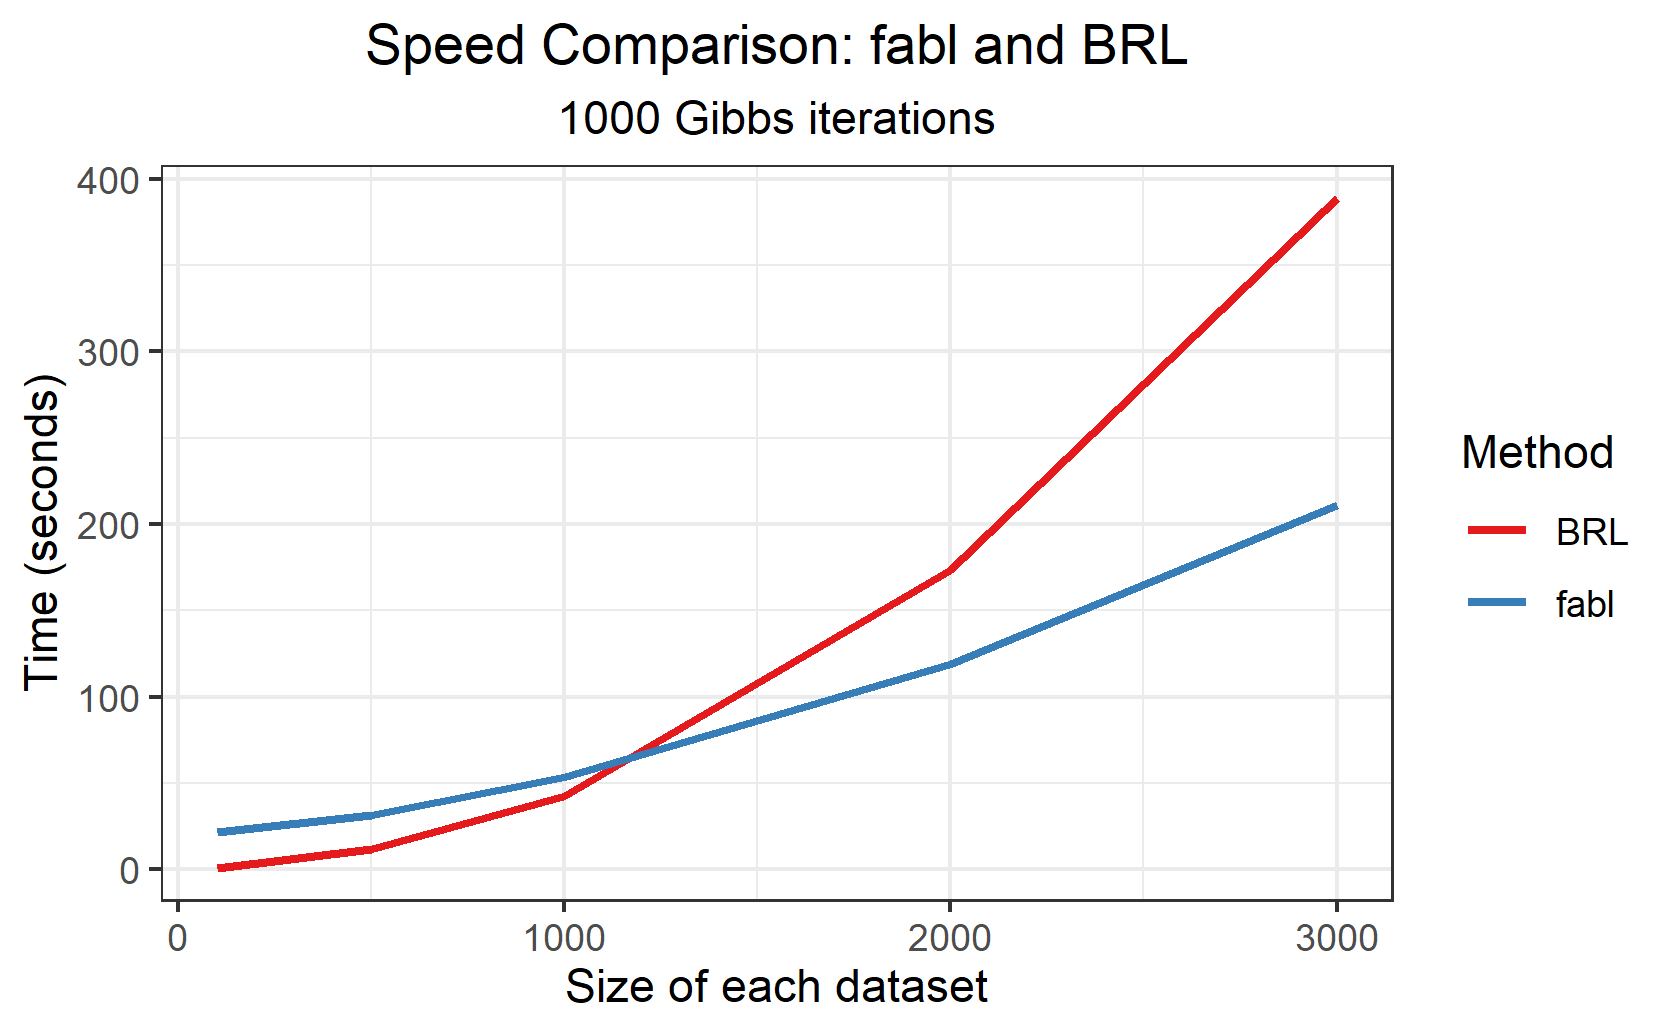
\includegraphics[width=0.6\textwidth]{../notes/figures/sadinle_speed_plot2} 
			\caption{Run-time for BRL and fabl to run 1000 Gibbs iterations, including hashing step for fabl, for increasing values of both $n_A$ and $n_B$. We see near quadratic growth in run-time for BRL, and near linear growth for fabl.}\label{fig:speed1}
		\end{center}
	\end{figure}
	
	The above discussion suggests that for fixed \(n_2\), computation time for \texttt{fabl} should remain mostly constant with growing \(n_1\). In the simulation results displayed in Figure~\ref{fig:speed2} fixing \(n_2 = 500\), we see linear growth for the run-time under \texttt{BRL} as \(n_1\) increases, with much more static run-time under \texttt{fabl}. The slight increases in run-time for \texttt{fabl} are due primarily to the hashing step, which again can be run in parallel for large data.
	
	\begin{figure}[h!]
		\begin{center} 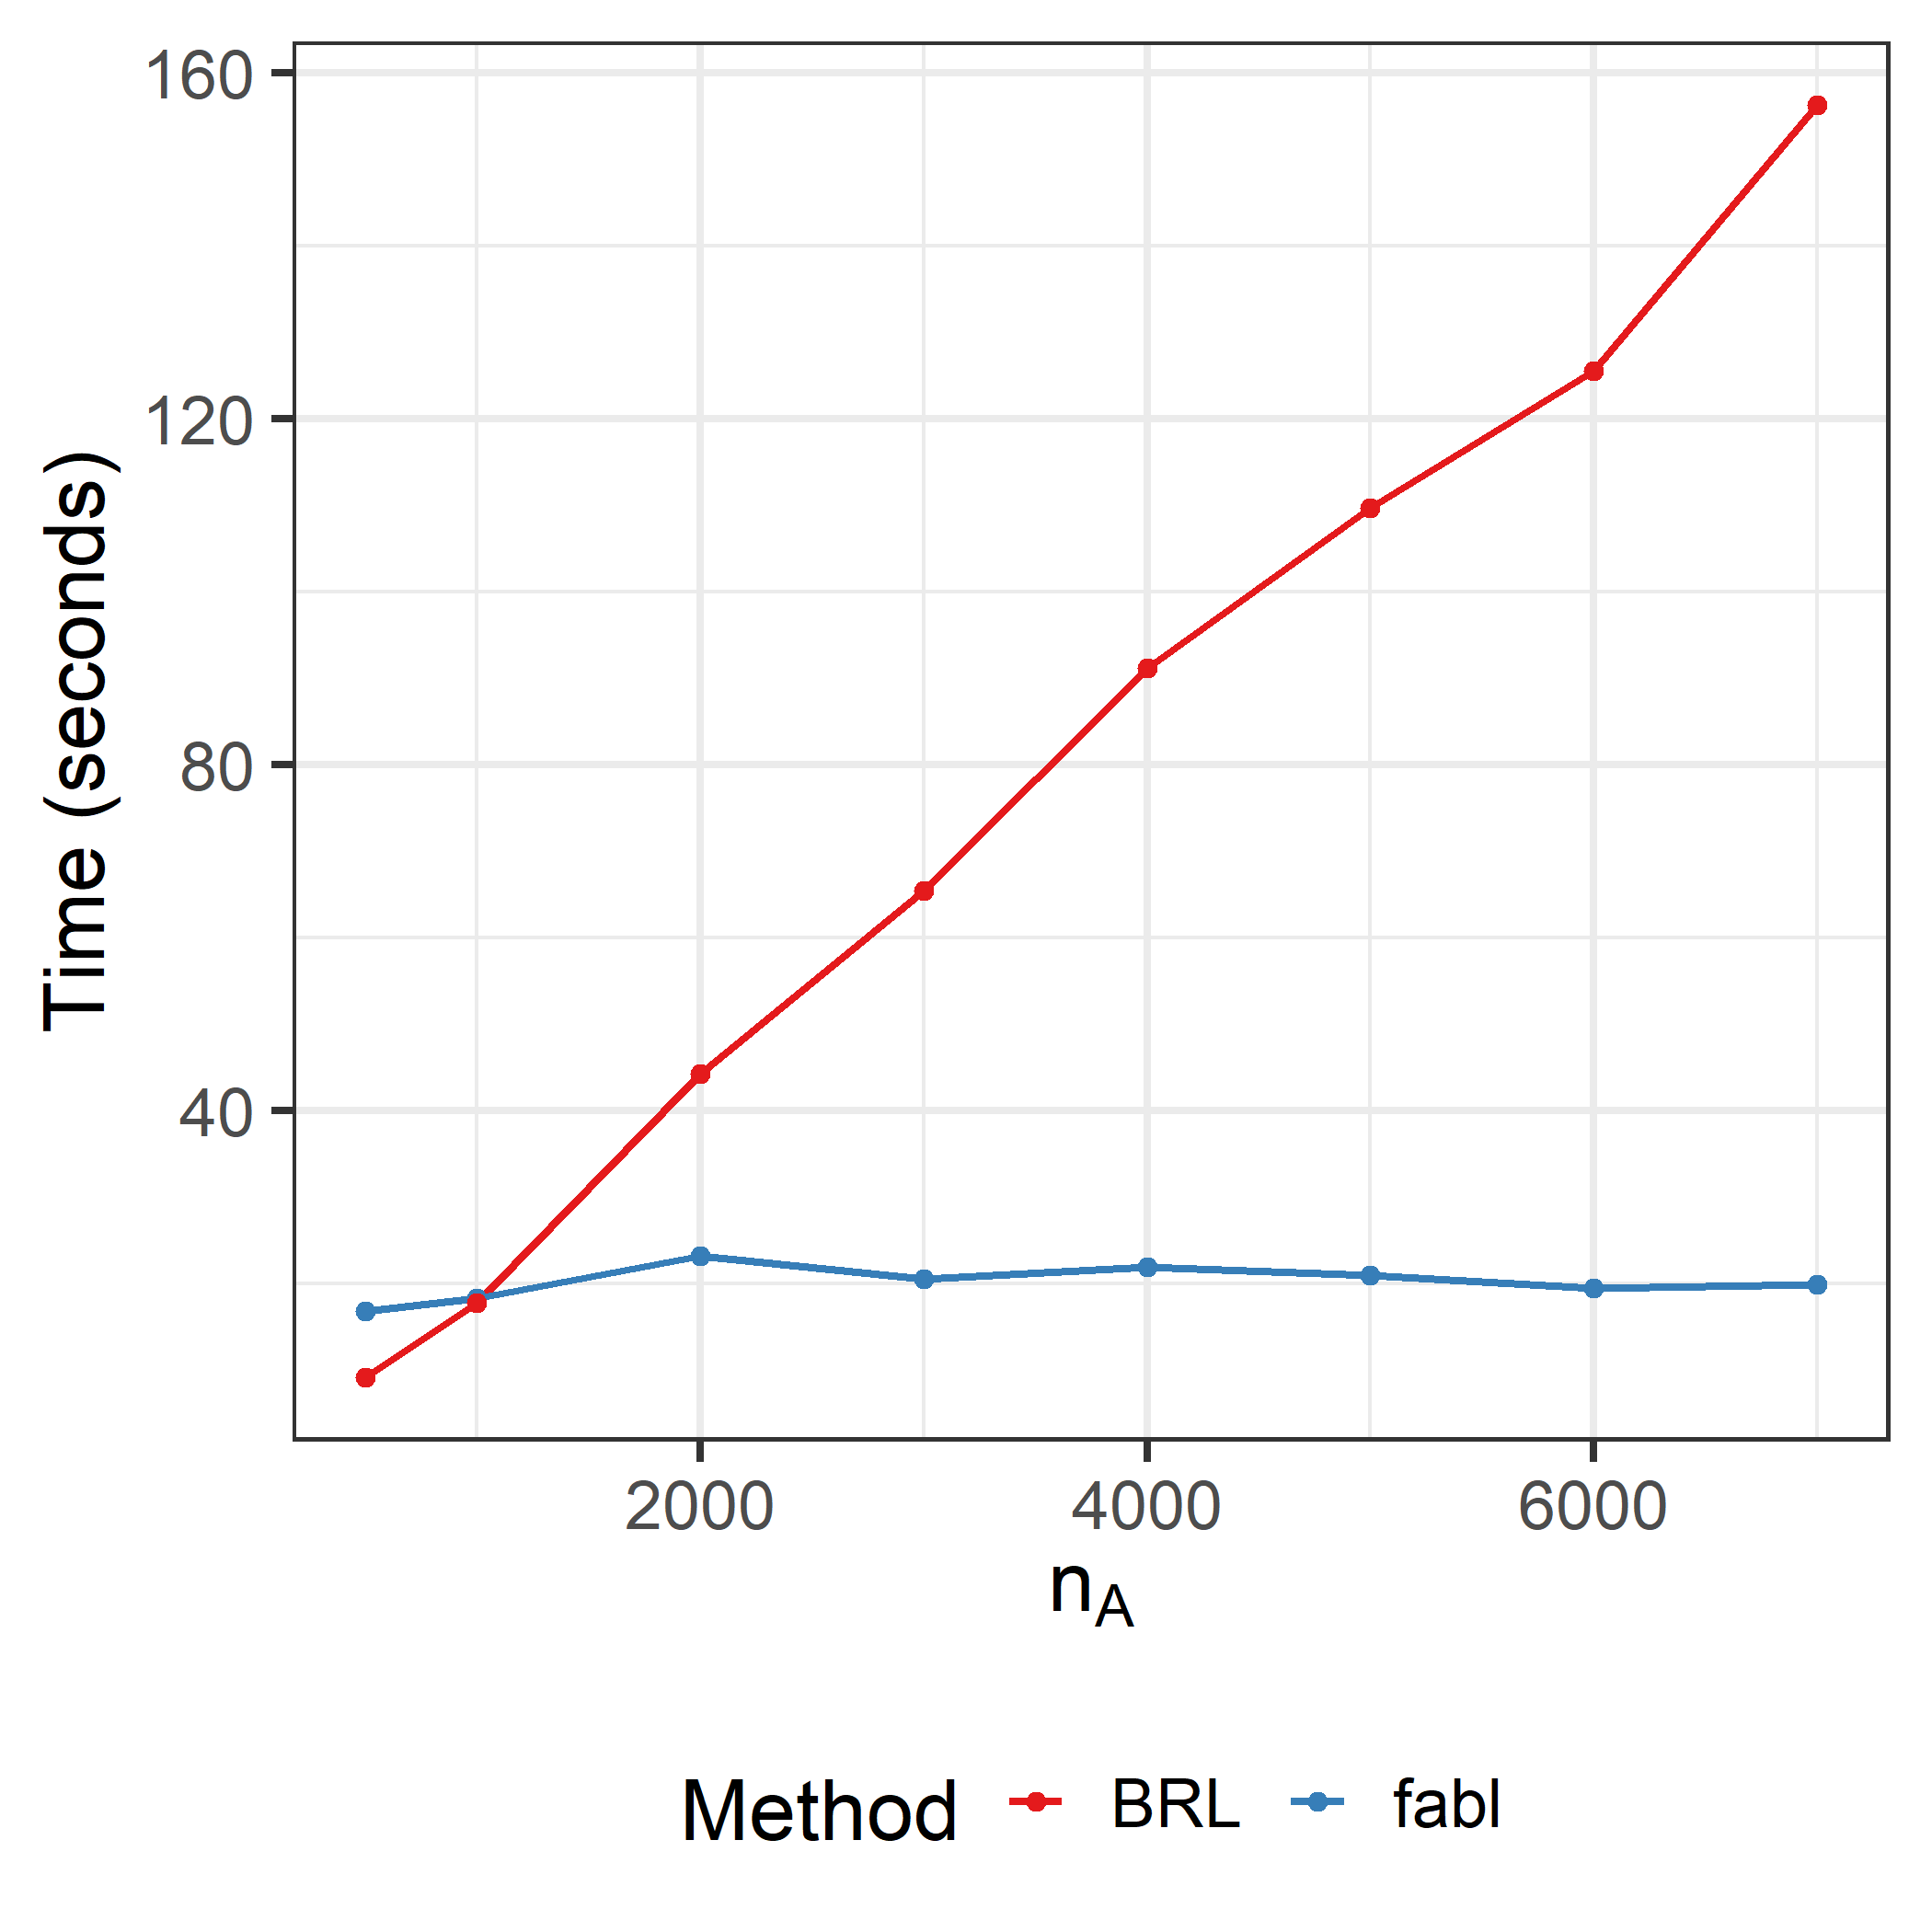
\includegraphics[width=0.6\textwidth]{../notes/figures/speed_plot_fixed_nB_slides} 
			\caption{Run-time for BRL and fabl to run 1000 Gibbs iterations, including hashing step for fabl, with increasing $n_A$, and $n_B$ fixed at 500. We see linear growth in run-time for BRL, and near constant run-time for fabl.}\label{fig:speed2}
		\end{center}
	\end{figure}
	
	
	\hypertarget{accuracy}{%
		\subsection{Accuracy under Full Estimates}\label{accuracy}}
	
	We replicate a simulation study from \cite{sadinle_bayesian_2017} to compare \texttt{fabl} against \texttt{BRL} on several synthetic datasets with varying amounts of error and overlap (the number of records in common across files). Following methods proposed by \cite{christen_pudjijono2009} and \cite{christen_vatsalan2013}, clean records are first simulated from frequency tables for first name, last name, age, and occupation in Australia. Fields are then chosen for distortion uniformly at random. Names are subject to string insertions, deletions and substitutions, as well as common keyboard, phonetic, and optical recognition errors. Age and occupation are distorted through keyboard errors and missingness.
	
	We create comparison vectors according to the default settings of the \texttt{compareRecords} function from the \texttt{BRL} package, shown in Table~\ref{Tab:sadinle_simulation_cutoffs}. Each simulation identifies matched individuals between two datasets, each with 500 records. We conduct linkage when matching records exhibit 1, 2, and 3 errors across the four fields, and when there are 50, 250, and 450 individuals in common across datasets. We use flat priors for all $m$ and $u$ parameters, run the Gibbs Sampler for 1000 iterations, and discard the first 100 as burn-in. We calculate Bayes estimates of the linkage structure using the losses $\theta_R = \infty, \theta_{10} = 1, \theta_{01} = 1, \theta_{11} = 2$. Traceplots for parameters of interest for one example simulation are provided in Appendix \ref{app:appendix-sim}; they show no obvious concern over MCMC convergence.
	
	\begin{table}[t]
		\centering
		\begin{tabular}[t]{llllll}
			
			\multicolumn{2}{c}{ } & \multicolumn{4}{c}{Level of Disagreement} \\
			\cline{3-6}
			Fields & Similarity & 1 & 2 & 3 & 4\\
			\hline
			First and Last Name & Levenstein & 0 & (0, .25] & (.25, .5] & (.5, .1]\\
			Age and Occupation & Binary & Agree & Disagree &  & \\
			\hline
		\end{tabular}
		\caption{Construction of comparison vectors for accuracy study with simulated datasets.}
		\label{Tab:sadinle_simulation_cutoffs}
	\end{table}
	
	We compare \texttt{fabl} to \texttt{BRL} in terms of recall, precision and F-measure, as defined in \cite{christen_2012}. Recall is the proportion of true matches found by the model, that is, $\sum_{j=1}^{n_2} I(\hat{Z}_j = Z_j, Z_j \leq n_1) / \sum_{j=1}^{n_2} I(Z_j \leq n_1)$. Precision is proportion of links found by the model that are true matches, that is $\sum_{j=1}^{n_2} I(\hat{Z}_j = Z_j, Z_j \leq n_1) / \sum_{j=1}^{n_2} I(\hat{Z}_j \leq n_1)$. The F-measure balances the two metrics to provide an overall measure of accuracy, and is defined as $2 \times (\text{Recall } + \text{ Precision}) / (\text{Recall } \times \text{ Precision})$. In Figure~\ref{fig:sadinle_simulation}, we see that the two methods have comparable performance at all levels of error and overlap. In the specific case of high error and low overlap, widely regarded as the most difficult linkage scenario, we see that \texttt{fabl} performs slightly worse on average; however, the overall accuracy level remains high. 
	
	
	%Each metric is provided explicitly below:
	%$$\text{Recall } = \frac{\sum_{j=1}^{n_2} I(\hat{Z}_j = Z_j, Z_j \leq n_1)}{\sum_{j=1}^{n_2} I(Z_j \leq n_1)}$$
	%$$\text{Precision } = \frac{\sum_{j=1}^{n_2} I(\hat{Z}_j = Z_j, Z_j \leq n_1)}{ \sum_{j=1}^{n_2} I(\hat{Z}_j \leq n_1)}$$
	%$$\text{F-measure } = 2 \frac{\text{Recall } + \text{Precision}}{\text{Recall } \times \text{Precision}}$$
	
	
	
	\begin{figure}[t]
		\begin{center}
			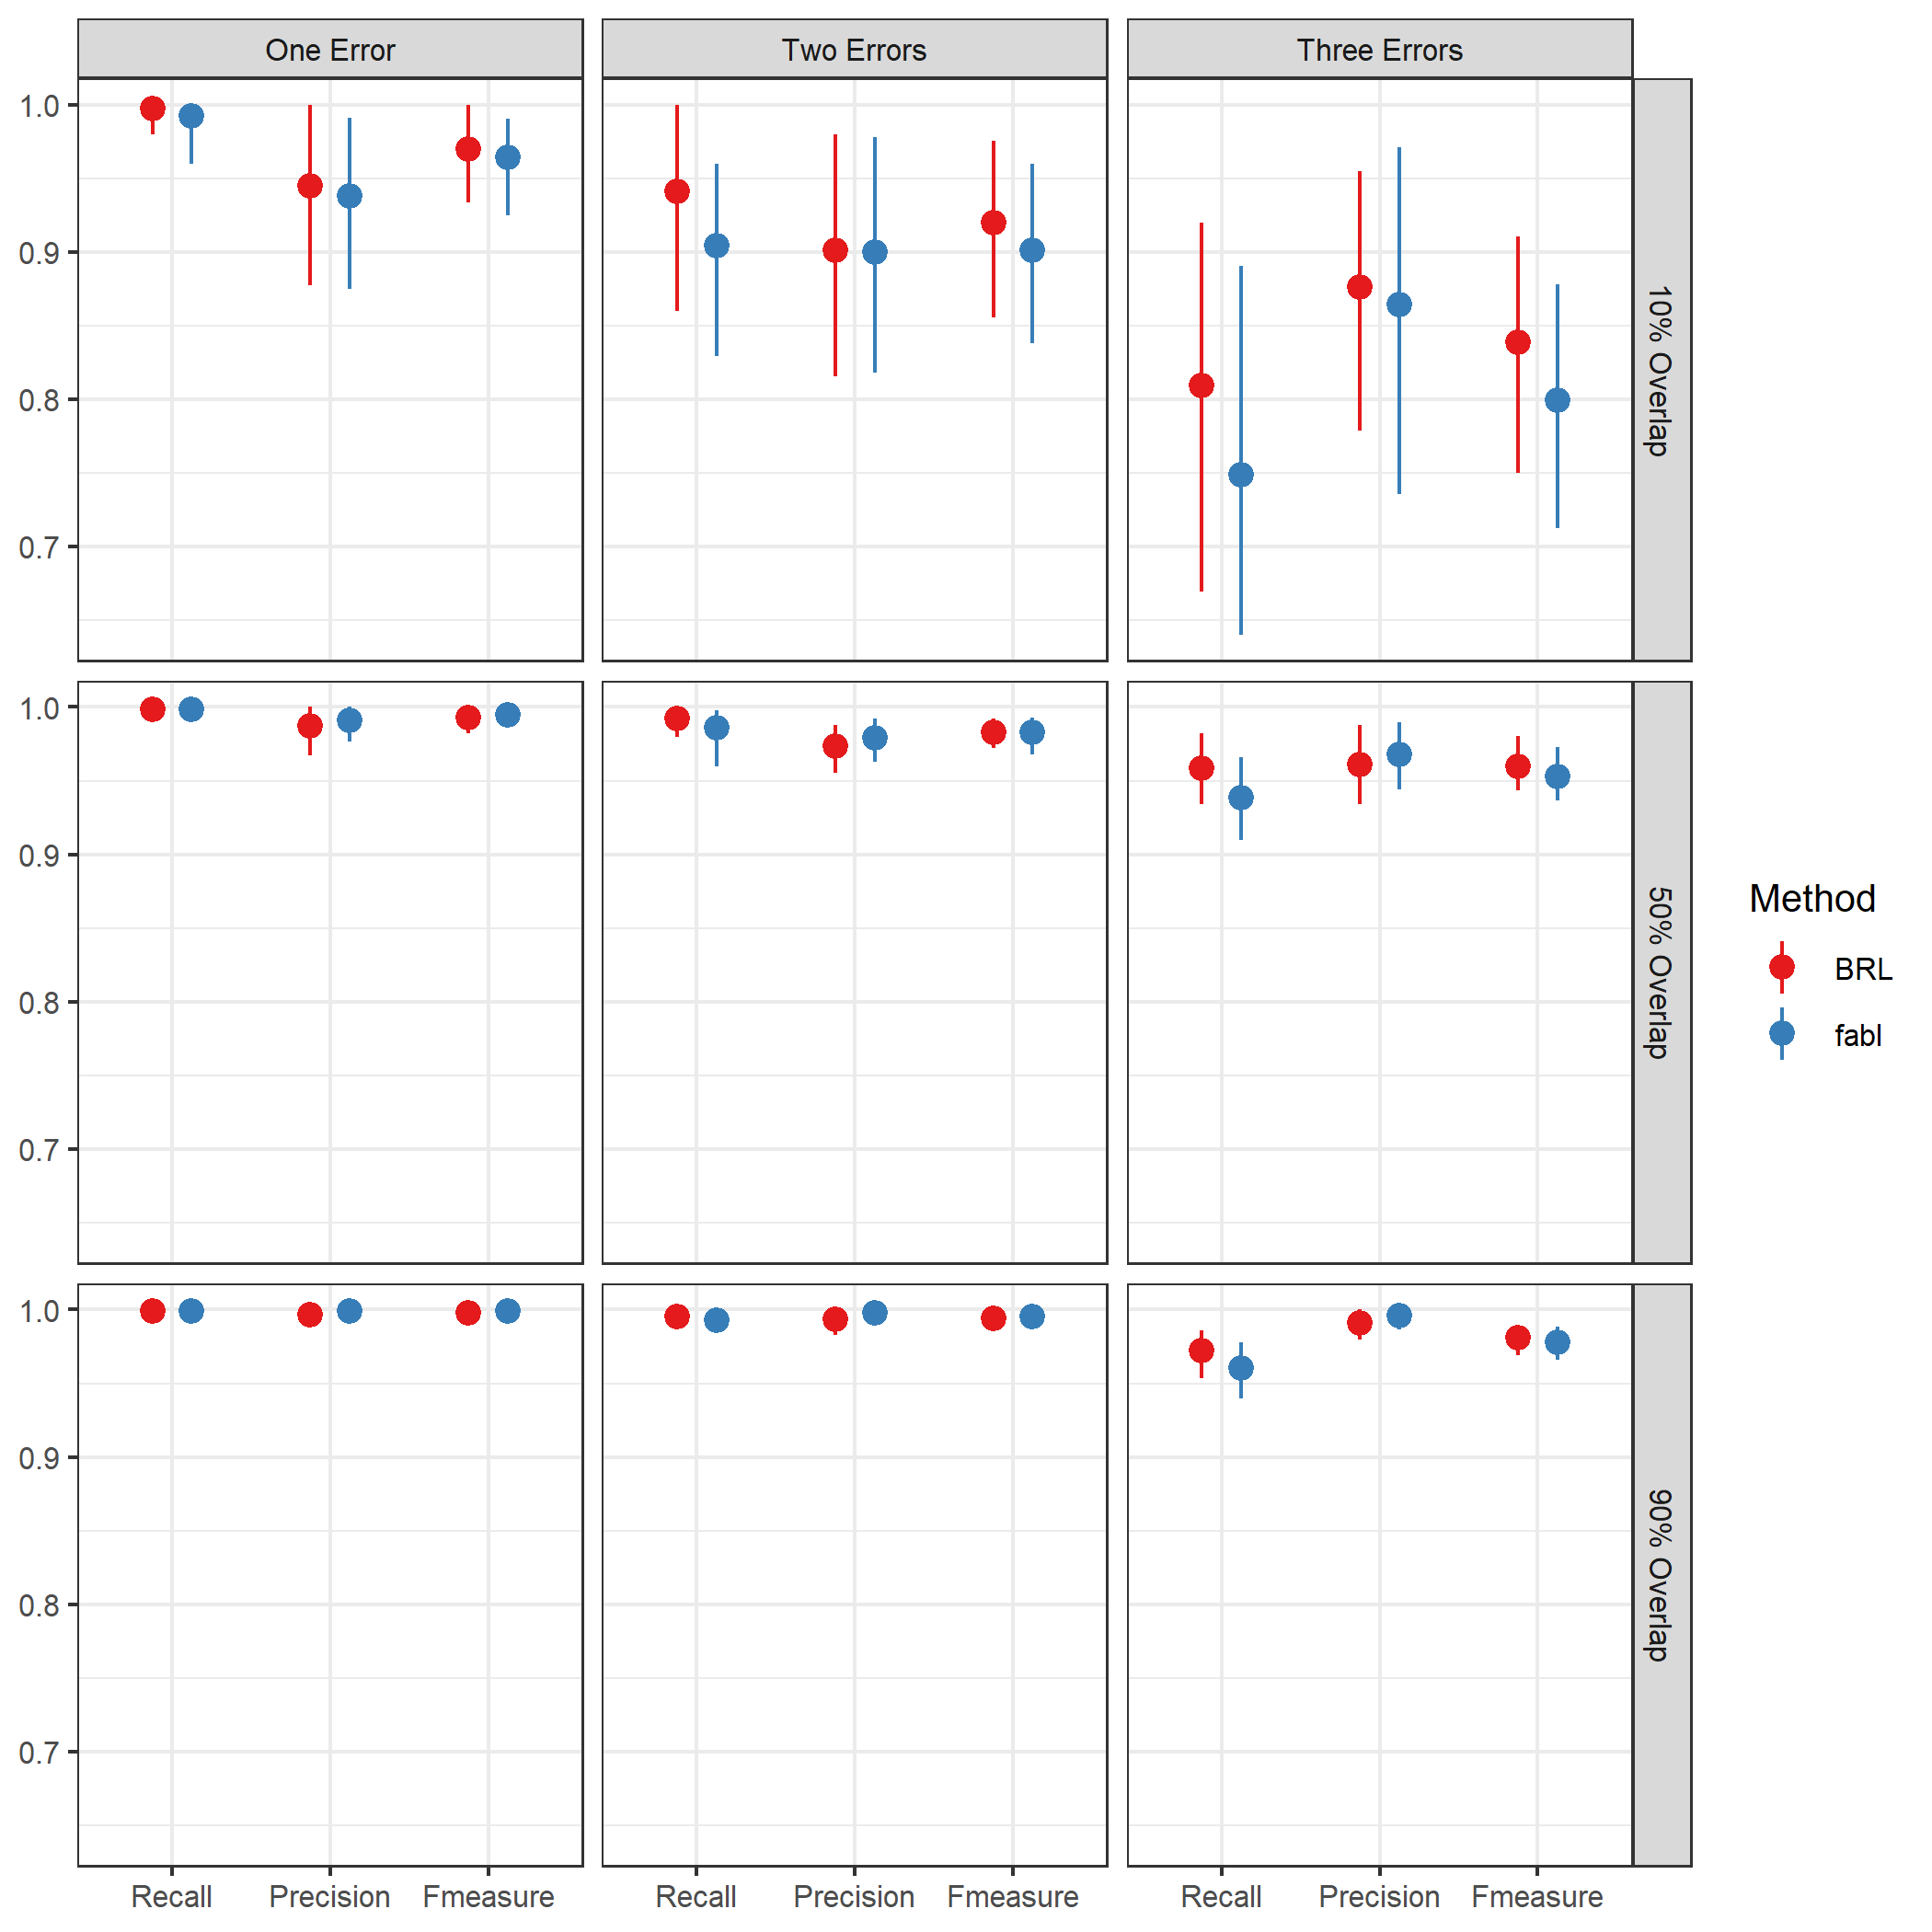
\includegraphics[width=0.6\textwidth]{../notes/figures/sadinle_sim_plot2} 
			\caption{Posterior means and credible intervals for accuracy metrics under the replication of simulation study from \cite{sadinle_bayesian_2017}. For each level of overlap and each level of error, we have 100 paired sets of 500 records. We see comparable performance for all levels of error and overlap.}
			\label{fig:sadinle_simulation}
		\end{center}
	\end{figure}
	
	\hypertarget{partial}{%
		\subsection{Accuracy under Partial Estimates}\label{partial}}
	
	By leaving $\theta_{10} = \theta_{01} = 1$ and $\theta_{11} = 2$, but setting $\theta_R = 0.1$, we allow the model to decline to decide a match for certain records, with nonassignment being 10\% as costly as a false match. In this context, we are no longer focused on finding all true matches, but rather protecting against false matches. Thus, instead of recall, we use the negative predictive value (NPV), defined as the proportion of non-links that are actual non-matches. Mathematically, $\text{NPV} = \sum_{j=1}^{n_2} I(\hat{Z}_j = Z_j = n_1 + j)$/$\sum_{j=1}^{n_2} I(\hat{Z}_j = n_1 + j)$. We continue to use the precision, which is renamed the positive predictive value (PPV) in this context. Lastly, we also report the rejection rate (RR), or how often the model declines to make a linkage decision, defined as RR = $\sum_{j=1}^{n_2} I(\hat{Z}_j = R)$.
	
	In Figure~\ref{fig:sadinle_simulation_partial}, we see that \texttt{fabl} maintains equivalently strong PPV as \texttt{BRL} across all linkage settings. However, with high amounts of error, and thus fewer accurate and discerning fields of information, the rejection rate under \texttt{fabl} rises, leading to a decrease in NPV. Since \texttt{fabl} does not remove previously matched records from consideration for a new record, posterior probabilities of matches at times can be split across more records; in contrast, \texttt{BRL} is able to maintain higher confidence in matches in this setting. If one wishes to use partial estimates, \texttt{fabl} will possibly leave more linkages for the modeller to match by hand than would be left under \texttt{BRL}, but the decisions made by each method will have nearly equal accuracy. 
	
	%In practice, it is rare to encounter linkage tasks with 90\% overlap, so we remain confident in \texttt{fabl}'s performance. If one wishes to use partial estimates, \texttt{fabl} will possibly leave more linkages for the modeller to match by hand that would be left under \texttt{BRL}, but the decisions made by each method will have nearly equal accuracy. 
	
	%This is reasonable because large numbers of errors blur the distinction between matched and non-matched pairs, leading to situations where one record in $\bf{X}_2$ has multiple plausible matches in $\bf{X}_1$, so that posterior match probability is split across more records.
	
	\begin{figure}[t]
		\begin{center}
			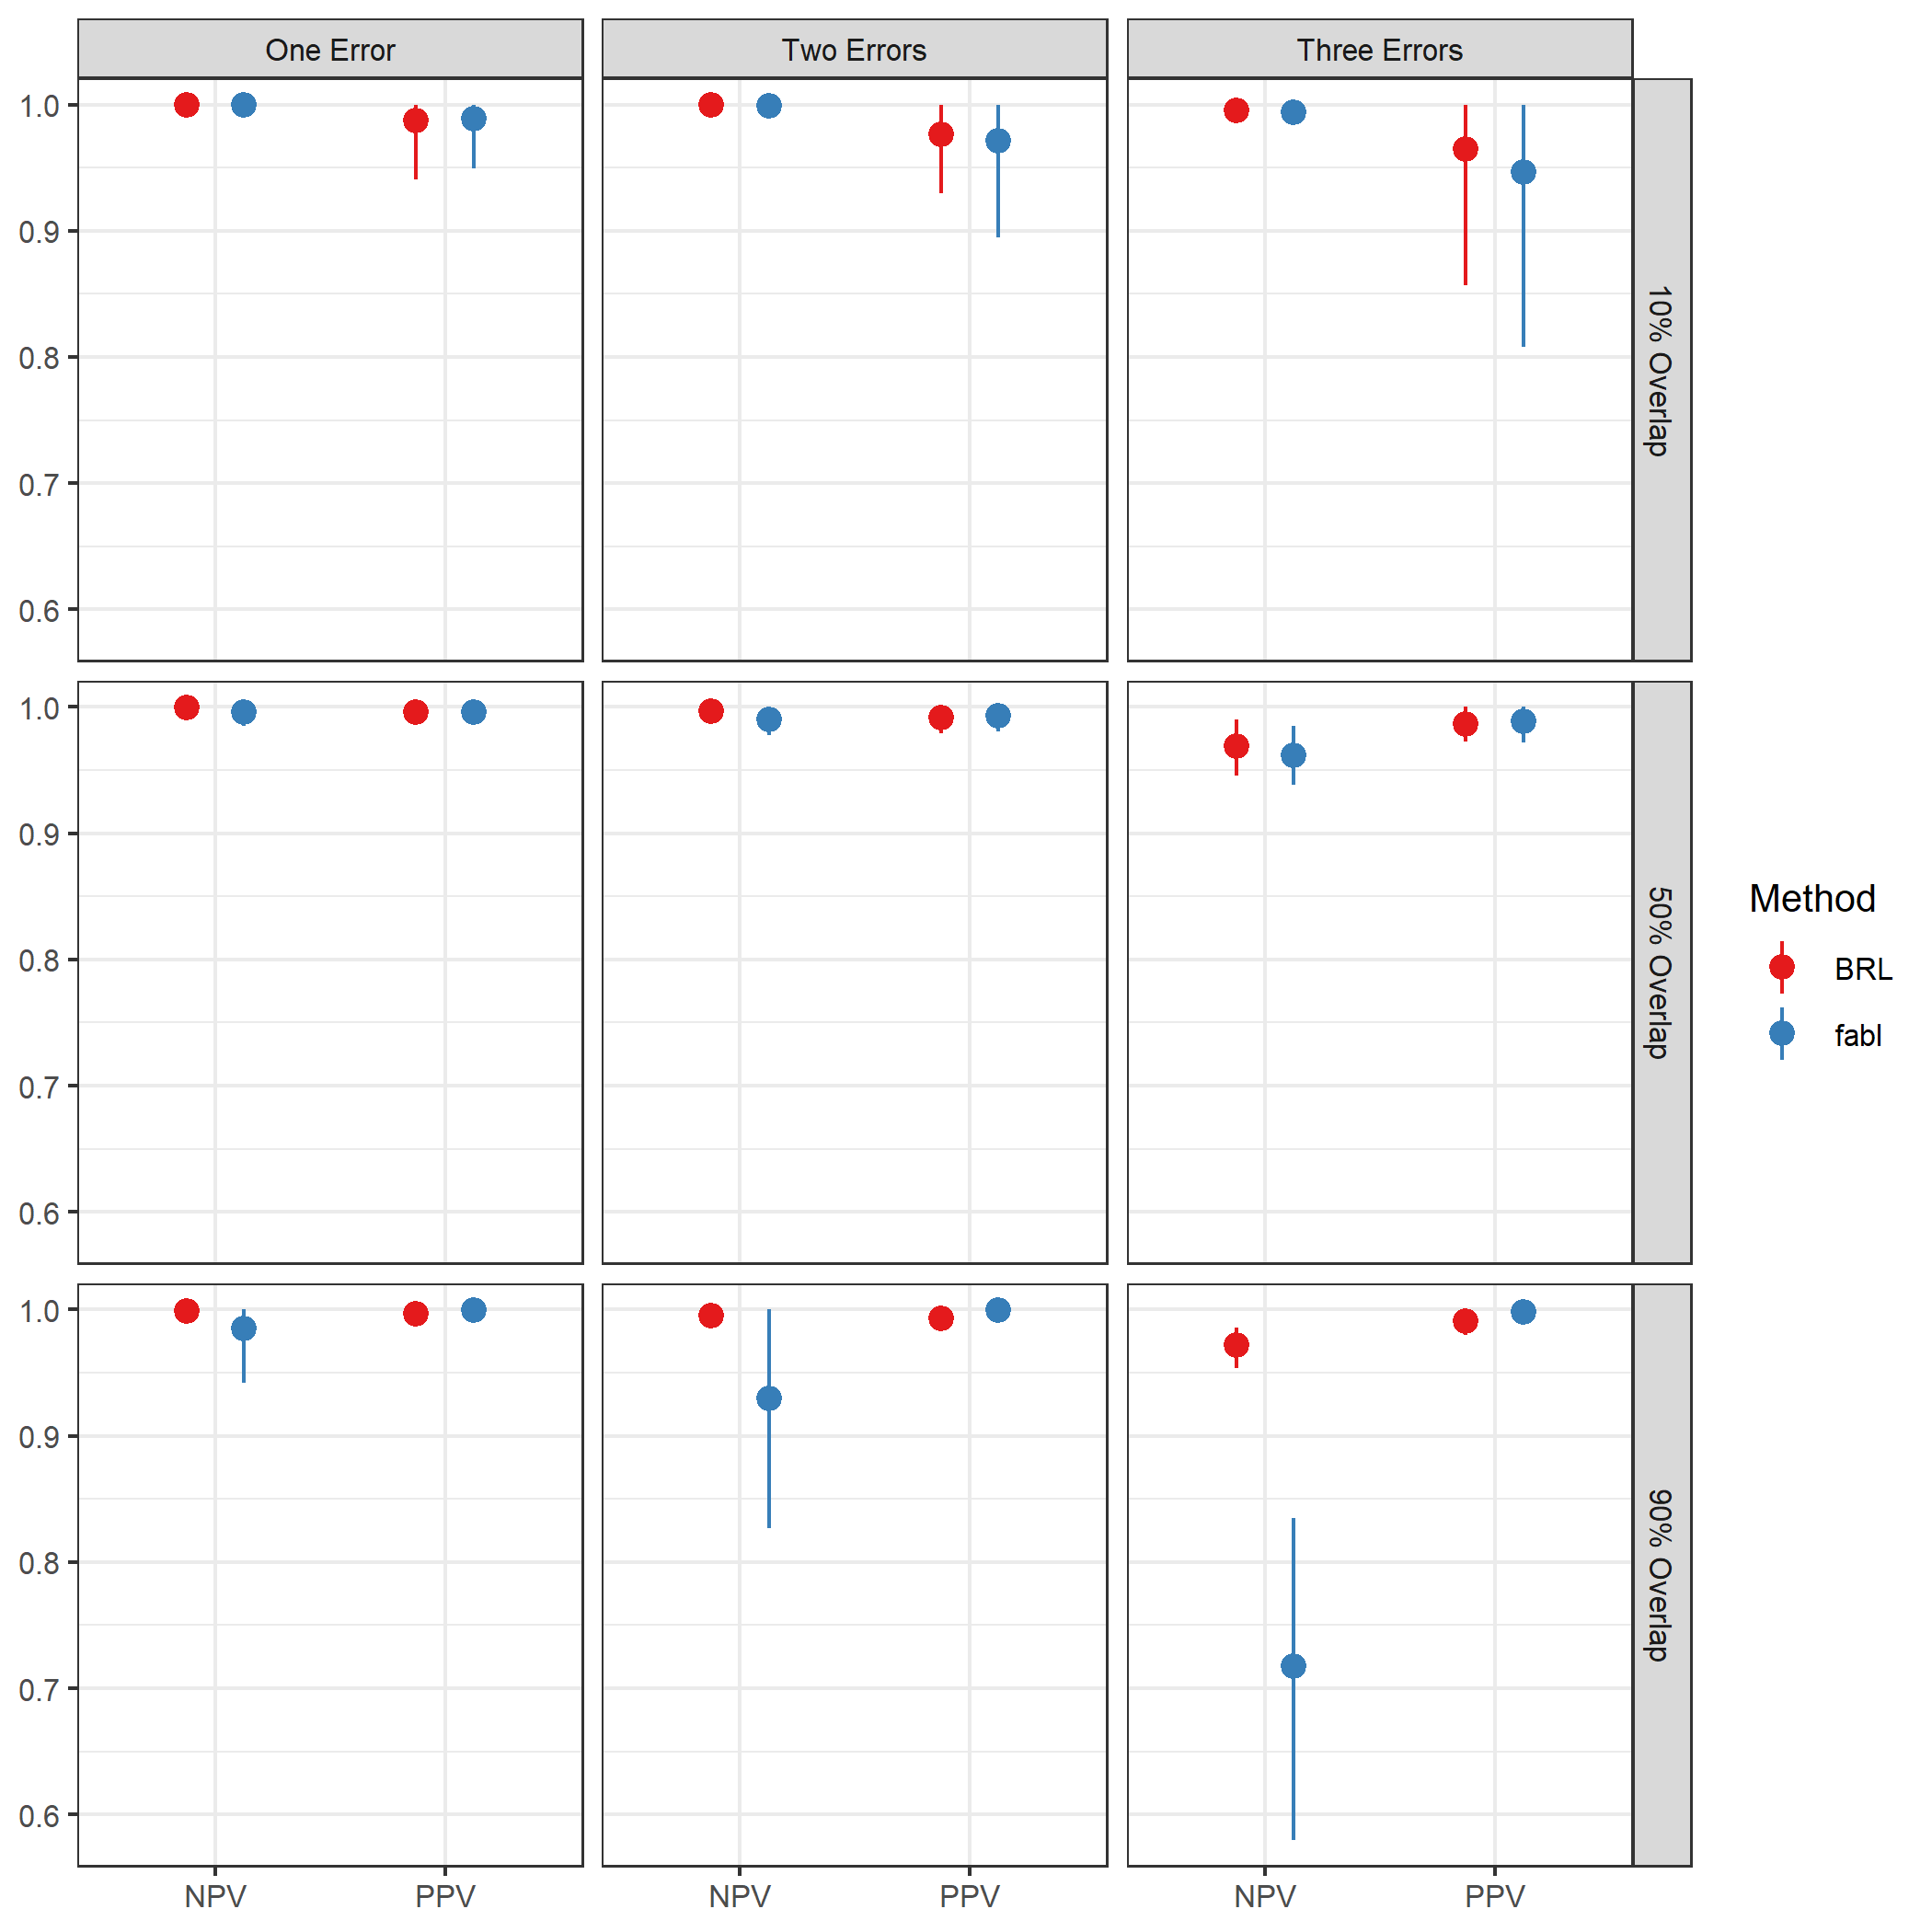
\includegraphics[width=0.6\textwidth]{../notes/figures/sadinle_sim_plot_partial} 
			\caption{Negative predictive value (NPV) and positive predictive value (PPV) on simulated datasets. We see poorer performance for \texttt{fabl} only in situations with high overlap.}
			\label{fig:sadinle_simulation_partial}
		\end{center}
	\end{figure}
	
	
	
	
	%\hypertarget{scale}{%
		%	\subsection{Scaling to a Larger Simulation Study}\label{scale}}
	%
	%To demonstrate the scale of the linkage tasks possible under \texttt{fabl}, we concatenate two sets of 40 simulated datasets from the original simulation studies of \cite{sadinle_bayesian_2017}, creating two larger files, each of 20,000 records (40,000 records total). Under standard Fellegi Sunter procedures, this would require 400,000,000 comparison vectors, each consisting for four integers, resulting in a final comparison matrix about 6.4 GB in size. Under default settings on a personal computer, \texttt{R} does not allow storing an object this size, so \texttt{BRL} is not usable on this linkage task. Through \texttt{fabl} however, using just one machine, we sequentially compare records across chunks, hash results, and then synthesize summary statistics for the entire simulation.  
	% 
	%For simplicity, we partition one dataset into 20 smaller chunks, and leave the second dataset fully intact. We compare records, hash results, and then synthesize summary statistics for all 20 chunk comparisons. The resulting data object is only 90 MB, about 1\% the size of the object required under the standard method. Executed sequentially, these comparisons and the Gibbs sampler take about one hour to run. However, this could be substantially sped up using distributed computing.
	%
	%Turning to evaluation metrics, this simulation achieved 96.5\% recall and 97.7\% precision, with an overall F-measure of 97.1\% F-measure. This is slightly worse performance than  in the smaller simulation studies; this is expected because it is naturally more difficult to link more records with the same amount of information. With more linkage fields, \texttt{fabl} maintains the high accuracy in Section~\ref{accuracy}. 
	
	\section{Case Studies}
	\label{sec:case-studies}
	
	In our first case study, we revisit data from the El Salvadoran Civil War analyzed by \cite{sadinle_bayesian_2017}. Though the data files used in this case study are small, it shows how the computational complexity of \texttt{fabl} depends on the number of unique agreement patterns found in the data, and how significant computational gains can be achieved by simplifying the construction of the comparison vectors. In the second case study, we apply \texttt{fabl} to link records from the National Long Term Care Study (NLTCS), a larger linkage task that is not feasible in reasonable time under \texttt{BRL} with typical computing setups. 
	
	\subsection{Civilian Casualties from the El Salvadoran Civil War}
	\label{el_salvador}
	
	The country of El Salvador was immersed in civil war from 1980 to 1991. Throughout the time, several organizations attempted to document casualties of the conflict. When estimating the total number of casualties, one cannot simply sum the numbers recorded by each organization, as it is likely that the same individuals are recorded in multiple casualty lists. This is an important step in estimating the total number of deaths from a conflict using multiple systems estimation \citep{lum2013applications}. We utilize lists of casualties from the war, one collected by El Rescate - Tutela Regal (ERTL) and another from the Salvadoran Human Rights Commission (CDHES, by its acronym in Spanish).\footnote{We thank the Human Rights Data Analysis Group (HRDAG) for granting access to this data.} The ERTL dataset consists of digitized denunciations that had been published throughout the conflict, and the CDHES dataset consists of casualties that had been reported directly to the organization \citep{howland2008rescate, ball2000salvadoran}. The ERTL required additional investigation before recording denunciations as human rights abuses, and reports to the CHDES were made shortly after the events occurred; thus, both datasets are thought to be fairly reliable.
	
	There are several challenges with these data. First, both datasets have been automatically digitized, which inherently leads to some degree of typographical error. Second, the only fields recorded are given name, last name, date of death, and place of death. It is relatively common for a parent and child to share the same given name, resulting in indistinguishable records for two different individuals. 
	
	%This last point nearly breaks the earlier mentioned assumption that there are no duplicates within files, and reveals a key difference between \texttt{BRL} and \texttt{fabl}.
	
	Following \cite{sadinle_bayesian_2017}, we utilize records that have non-missing entries for given and last name, which results in \(n_1 = 4420\) records in CHDES and \(n_2 = 1323\) records in ERTL. We standardize names to account for common misspellings and use a modified Levenstein distance when comparing names to account for the fact that second names are often omitted in Spanish. Place of death is recorded by municipality and department within that municipality; however, since department is missing in 95\% of records in CHDES and 80\% of records in ERTL, we exclude department from our analysis. Thus, we conduct record linkage using given name, last name, municipality, and day, month, and year of death. We again use flat priors for the \(\bm{m}\) and \(\bm{u}\) parameters.
	
	\cite{sadinle_bayesian_2017} constructs the comparison vectors using four levels of agreement for each field, according to the thresholds provided in Table~\ref{Tab:el_salvador_cutoffs_1}. This results in \(4^5 \times 2 = 2048\) possible agreement patterns, with 1173 patterns realized in the data. We initially used these comparisons to estimate fabl and BRL.  However, after investigating the posterior distributions of the $\bm{m}$ and $\bm{u}$ parameters, we noticed that posterior distributions of several levels of the m and u parameters are nearly identical, suggesting that these levels are unnecessary for meaningfully modeling the distribution of the comparison vectors. 
	
	%However, we observed that posterior distributions of several levels of the \(\bm{m}\) and \(\bm{u}\) parameters were nearly identical, suggesting that the number of levels used are unnecessary for meaningfully representing the data.
	
	%here, the number of patterns was sufficiently high enough that the computational savings from \texttt{fabl} does not overcome the inherent speed differences of C as opposed to \texttt{R}.
	
	\begin{table}
		\begin{tabular}[t]{llllll}
			\hline
			\multicolumn{2}{c}{ } & \multicolumn{4}{c}{Level of Disagreement} \\
			\cline{3-6}
			Fields & Similarity & 1 & 2 & 3 & 4\\
			\hline
			First and Last Name & Modified Levenstein & 0 & (0, .25] & (.25, .5] & (.5, 1]\\
			Year of Death & Absolute Difference & 0 & 1 & 2 & 3+\\
			Month of Death & Absolute Difference & 0 & 1 & 2-3 & 4+\\
			Day of Death & Absolute Difference & 0 & 1-2 & 3-7 & 8+\\
			Municipality & Binary & Agree & Disagree &  & \\
			\hline
		\end{tabular}
		\caption{Construction of comparison vectors for El Salvador data resembling original implementation from \citep{sadinle2018bayesian}. This set up leads to 2048 possible agreement patterns in total.}\label{Tab:el_salvador_cutoffs_1}
	\end{table}
	
	Therefore we re-ran our analysis with fewer agreement levels for each field according to Table~\ref{Tab:el_salvador_cutoffs_2}. Among the 216 possible agreement patterns, 159 are realized in the data. With this revised comparison specification, fabl ran in 61 seconds, approximately 4 times faster than BRL 239 second run time.  The estimates of the $\bm{m}$ parameters under each method are very similar, as shown in Figure~\ref{fig:m-and-u}. Traceplots for parameters of interest are provided in Appendix \ref{app:appendix-es}.
	
	For completeness, we note that the more detailed comparison vector produced a run time of 240 seconds for BRL, and 261 seconds for fabl.  Apparently, the number of patterns was sufficiently many that the computational savings from fabl does not overcome the inherent speed differences of C as opposed to R.
	
	\begin{table}
		\centering
		\begin{tabular}[t]{lllll}
			\hline
			\multicolumn{2}{c}{ } & \multicolumn{3}{c}{Level of Disagreement} \\
			\cline{3-5}
			Fields & Similarity & 1 & 2 & 3\\
			\hline
			First and Last Name & Modified Levenstein & 0 & (0, .25] & (.25, 1]\\
			Year of Death & Binary & Agree & Disagree & \\
			Month of Death & Binary & Agree & Disagree & \\
			Day of Death & Absolute Difference & 0 & 1 & 2+\\
			Municipality & Binary & Agree & Disagree & \\
			\hline
		\end{tabular}
		\caption{Construction of comparison vectors for El Salvador for increased speed under \texttt{fabl}. This set up leads to 216 possible agreement patterns in total.}\label{Tab:el_salvador_cutoffs_2}
	\end{table}
	
	Through \texttt{fabl}, we arrive at a Bayes estimate of 179 individuals recorded in both datasets. We calculate posterior samples of the size of the overlap across files by finding the number of matches found in each iteration of the Gibbs sampler, and subtracting the number of matches that violate one-to-one matching. The posterior 95\% credible interval for the overlap across files is (206, 238), indicating that the Bayes estimate identifies fewer matches than the Gibbs sampler identifies on average. This is because a large number of records in ERTL have multiple plausible matches in CDHES; \texttt{fabl} recognizes that a match exists among the several options, but is unable to definitely declare a specific pair as a match in the Bayes estimate. We also compute a partial estimate of the linkage structure, using $\theta_{10} = \theta_{01} = 1$, $\theta_{11} = 2$, and $\theta_R = 0.1$ as in the simulation study in Section ~\ref{accuracy}. Here, the Bayes estimate provides 136 matches of which the model is quite confident, and 175 records to verify manually. This means that after clerical review, the number of individuals replicated across datasets would fall in the interval (136, 311), encapsulating the posterior credible interval. More or fewer records could be identified for clerical review by decreasing or increasing $\theta_R$. 
	
	We see similar results under \texttt{BRL}, with a Bayes estimate of 181 individuals recorded in both datasets, a posterior 95\% credible interval of (211, 244), and a range of (140, 294) after the partial estimate and clerical review. We note that Bayes estimates falling outside of posterior credible intervals has occurred previously in the record linkage literature \citep{sadinle_bayesian_2017, steorts_bayesian_2016}, and remains a topic for future research.
	
	We note that reconciling Bayes estimates that fall outside of posterior credible intervals is a common challenge in record linkage and an avenue of future work. 
	
	\begin{figure}[t]
		\begin{center}
			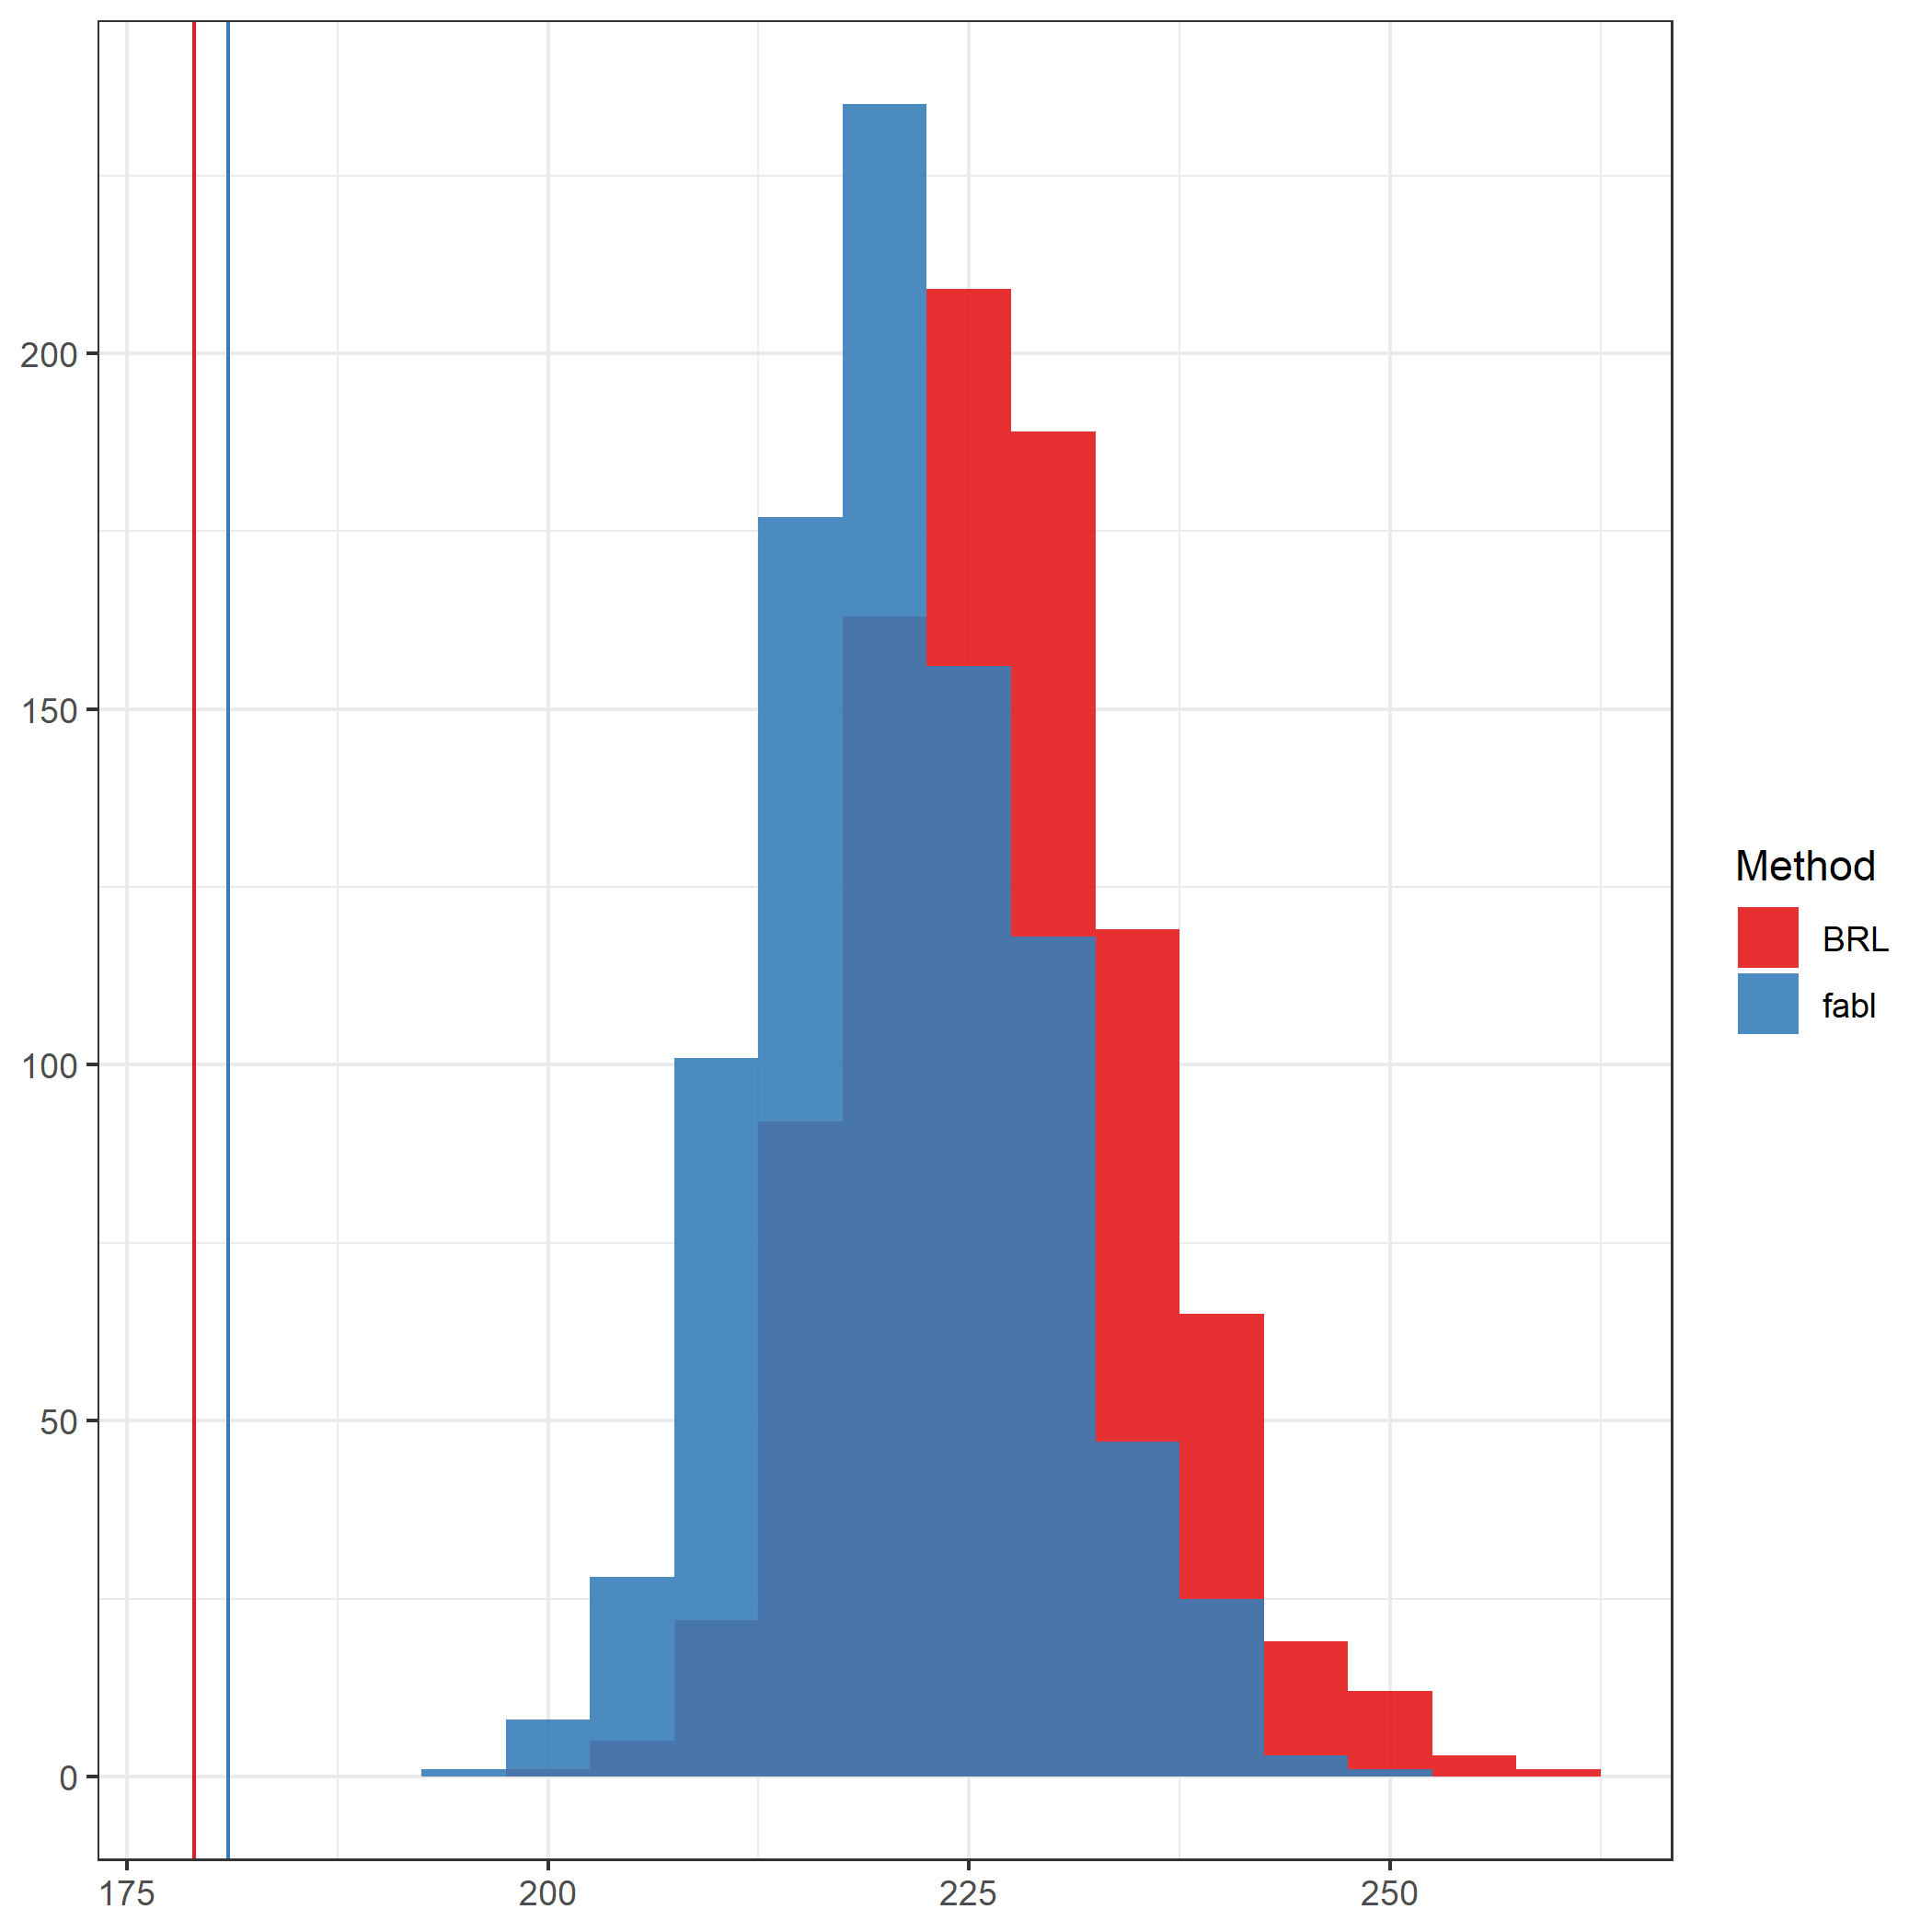
\includegraphics[width=0.6\textwidth]{../notes/figures/el_salvador/overlap_distribution_smallP_bayes}
			\caption{Posterior distribution and Bayes estimate of overlap across the two files. We note they are quite similar under both methods.}
			\label{fig:overlap-plot}
		\end{center}
	\end{figure}
	
	
	\begin{figure}[t]
		\begin{center}
			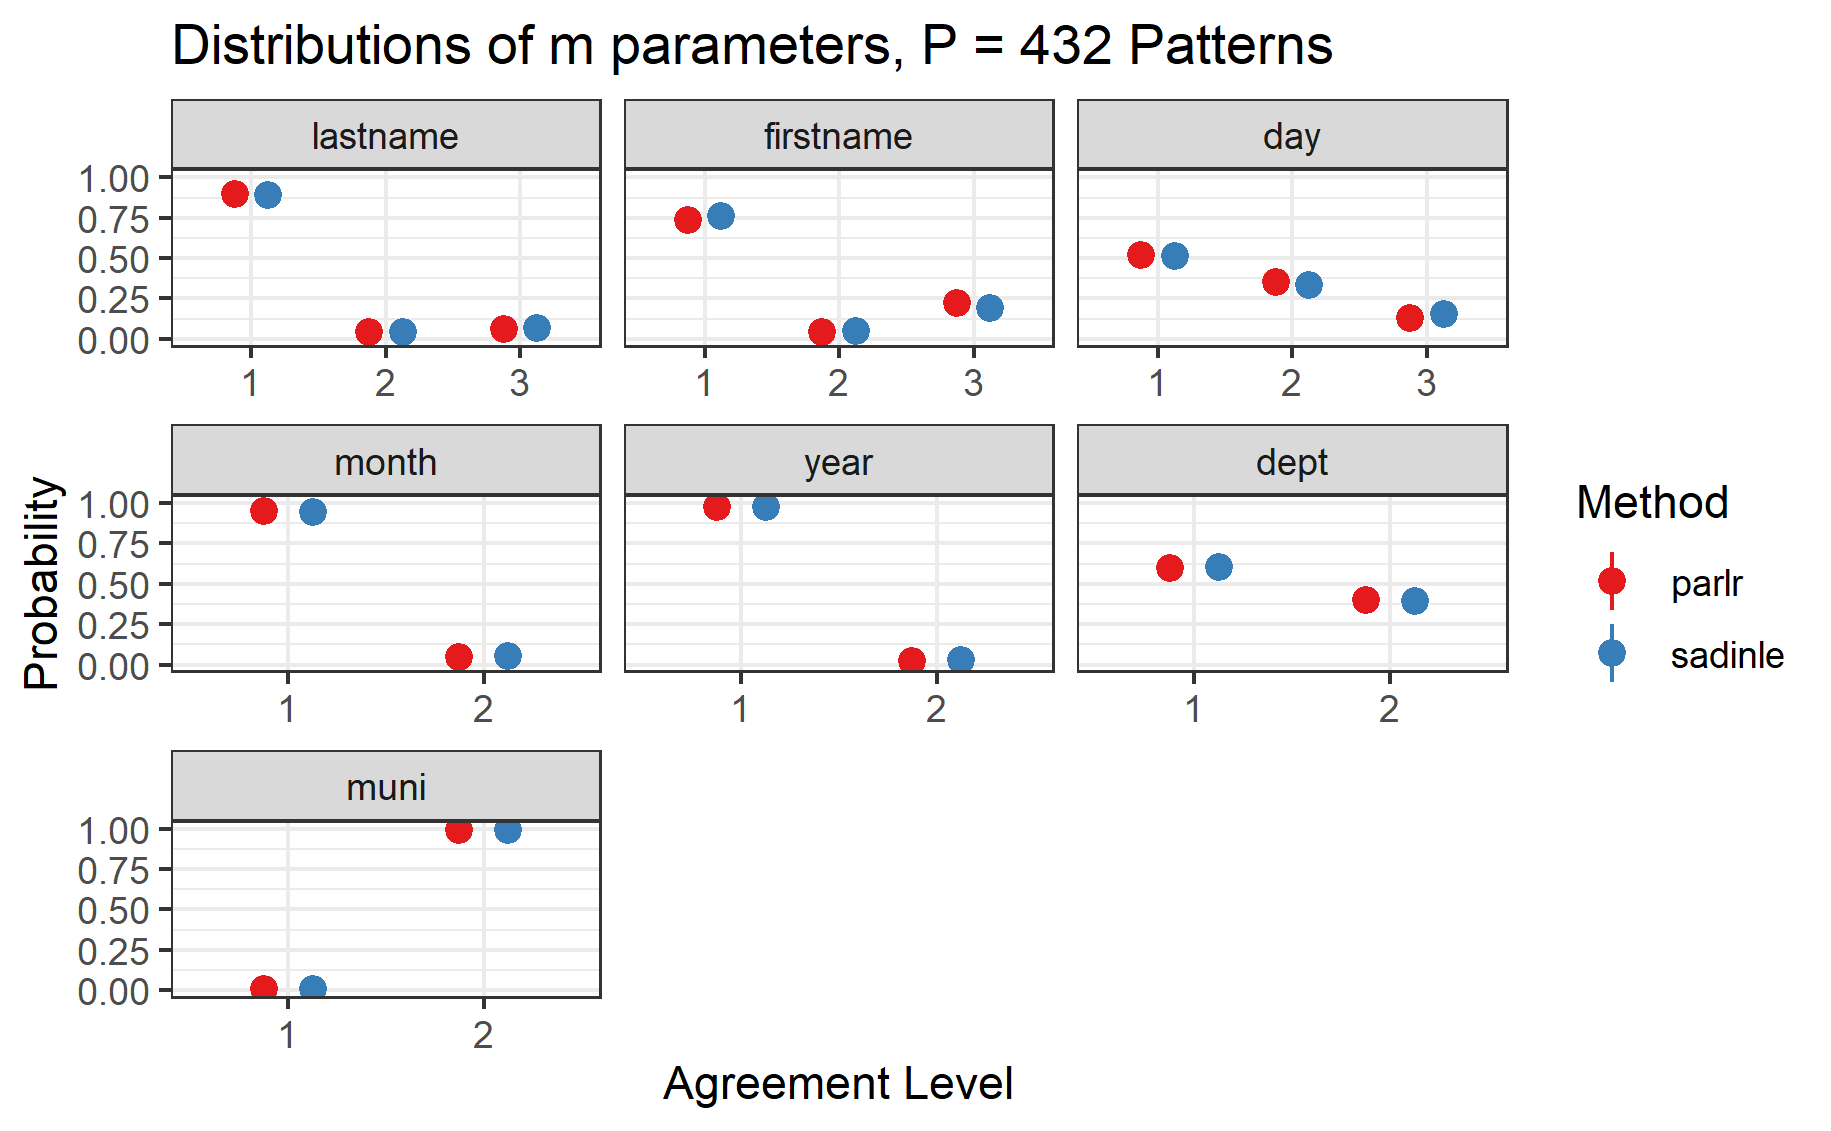
\includegraphics[width=0.6\textwidth]{../notes/figures/el_salvador/m_posterior_smallP} 
			\caption{Posterior estimates of m parameters with 95\% credible intervals for El Salvador case study. They are quite similar across the two methods.}\label{fig:m-and-u}
			\label{fig:m-and-u}
		\end{center}
	\end{figure}
	
	\subsection{National Long Term Care Study}
	\label{nltcs}
	
	The National Long Term Care Study (NLTCS) is a longitudinal study tracking the health outcomes of Medicare recipients. The initial began in 1982, with follow-up surveys taken approximately every five years. For this study, we seek to link records over the $n_A = 20485$ records from 1982 to the $n_B = 17466$ records from 1989. The NLTCS data have longitudinal links, so that in reality one does not need to do a record linkage.  However, following the strategy in \cite{guha:reiter:BA} we break the longitudinal links and treat the data from 1982 and 1989 as stand-alone files.
	
	We link records using sex, date of birth, and location using the thresholds shown in Table~\ref{Tab:nltcs-comparisons}. Storing five comparison scores for each of $20485 \times 17466 \approx 400,000,000$ record pairs would require approximately 8GB of memory. Standard settings on a 16GB personal computer do not allow storage of an object of this size, and thus \texttt{BRL} is unable to perform this linkage task on such a machine. However, through the \texttt{fabl} framework, we compute comparisons over 30 smaller comparison tasks, hash results, and compress information through storage efficient indexing; the resulting data object is just 10 MB, approximately 0.1\% of what is required for the raw comparisons. Constructing the comparisons sequentially took approximately 40 minutes, which could be reduced considerably through parallel computing. 
	
	We run a Gibbs sampler for 1000 iterations, taking about 235 seconds. The Bayes estimate of the linkage structure consists of 9634 matches, with a 95\% credible interval of (9581, 9740). Since we have access to the true linkage structure, we can calculate recall to be 0.89 and precision to be 0.98, resulting in an F-measure of 0.94. Traceplots indicate quick convergence, and are similar to those seen in Appendix \ref{app:appendix-sim} and \ref{app:appendix-es}
	
	\begin{table}
		\centering
		\begin{tabular}[t]{lllll}
			\hline
			\multicolumn{2}{c}{ } & \multicolumn{3}{c}{Level of Disagreement} \\
			\cline{3-5}
			Fields & Similarity & 1 & 2 & 3\\
			\hline
			Sex & Binary & Agree & Disagree & \\
			Year of Birth & Binary & Agree & Disagree & \\
			Month of Birth & Binary & Agree & Disagree & \\
			Day of Birth & Binary & Agree & Disagree & \\
			Location & Custom & Same State and Office & Same State & Otherwise \\
			\hline
		\end{tabular}
		\caption{Construction of comparison vectors for NTLCS data}\label{Tab:nltcs-comparisons}
	\end{table}
	
	\begin{figure}[t]
		\begin{center}
			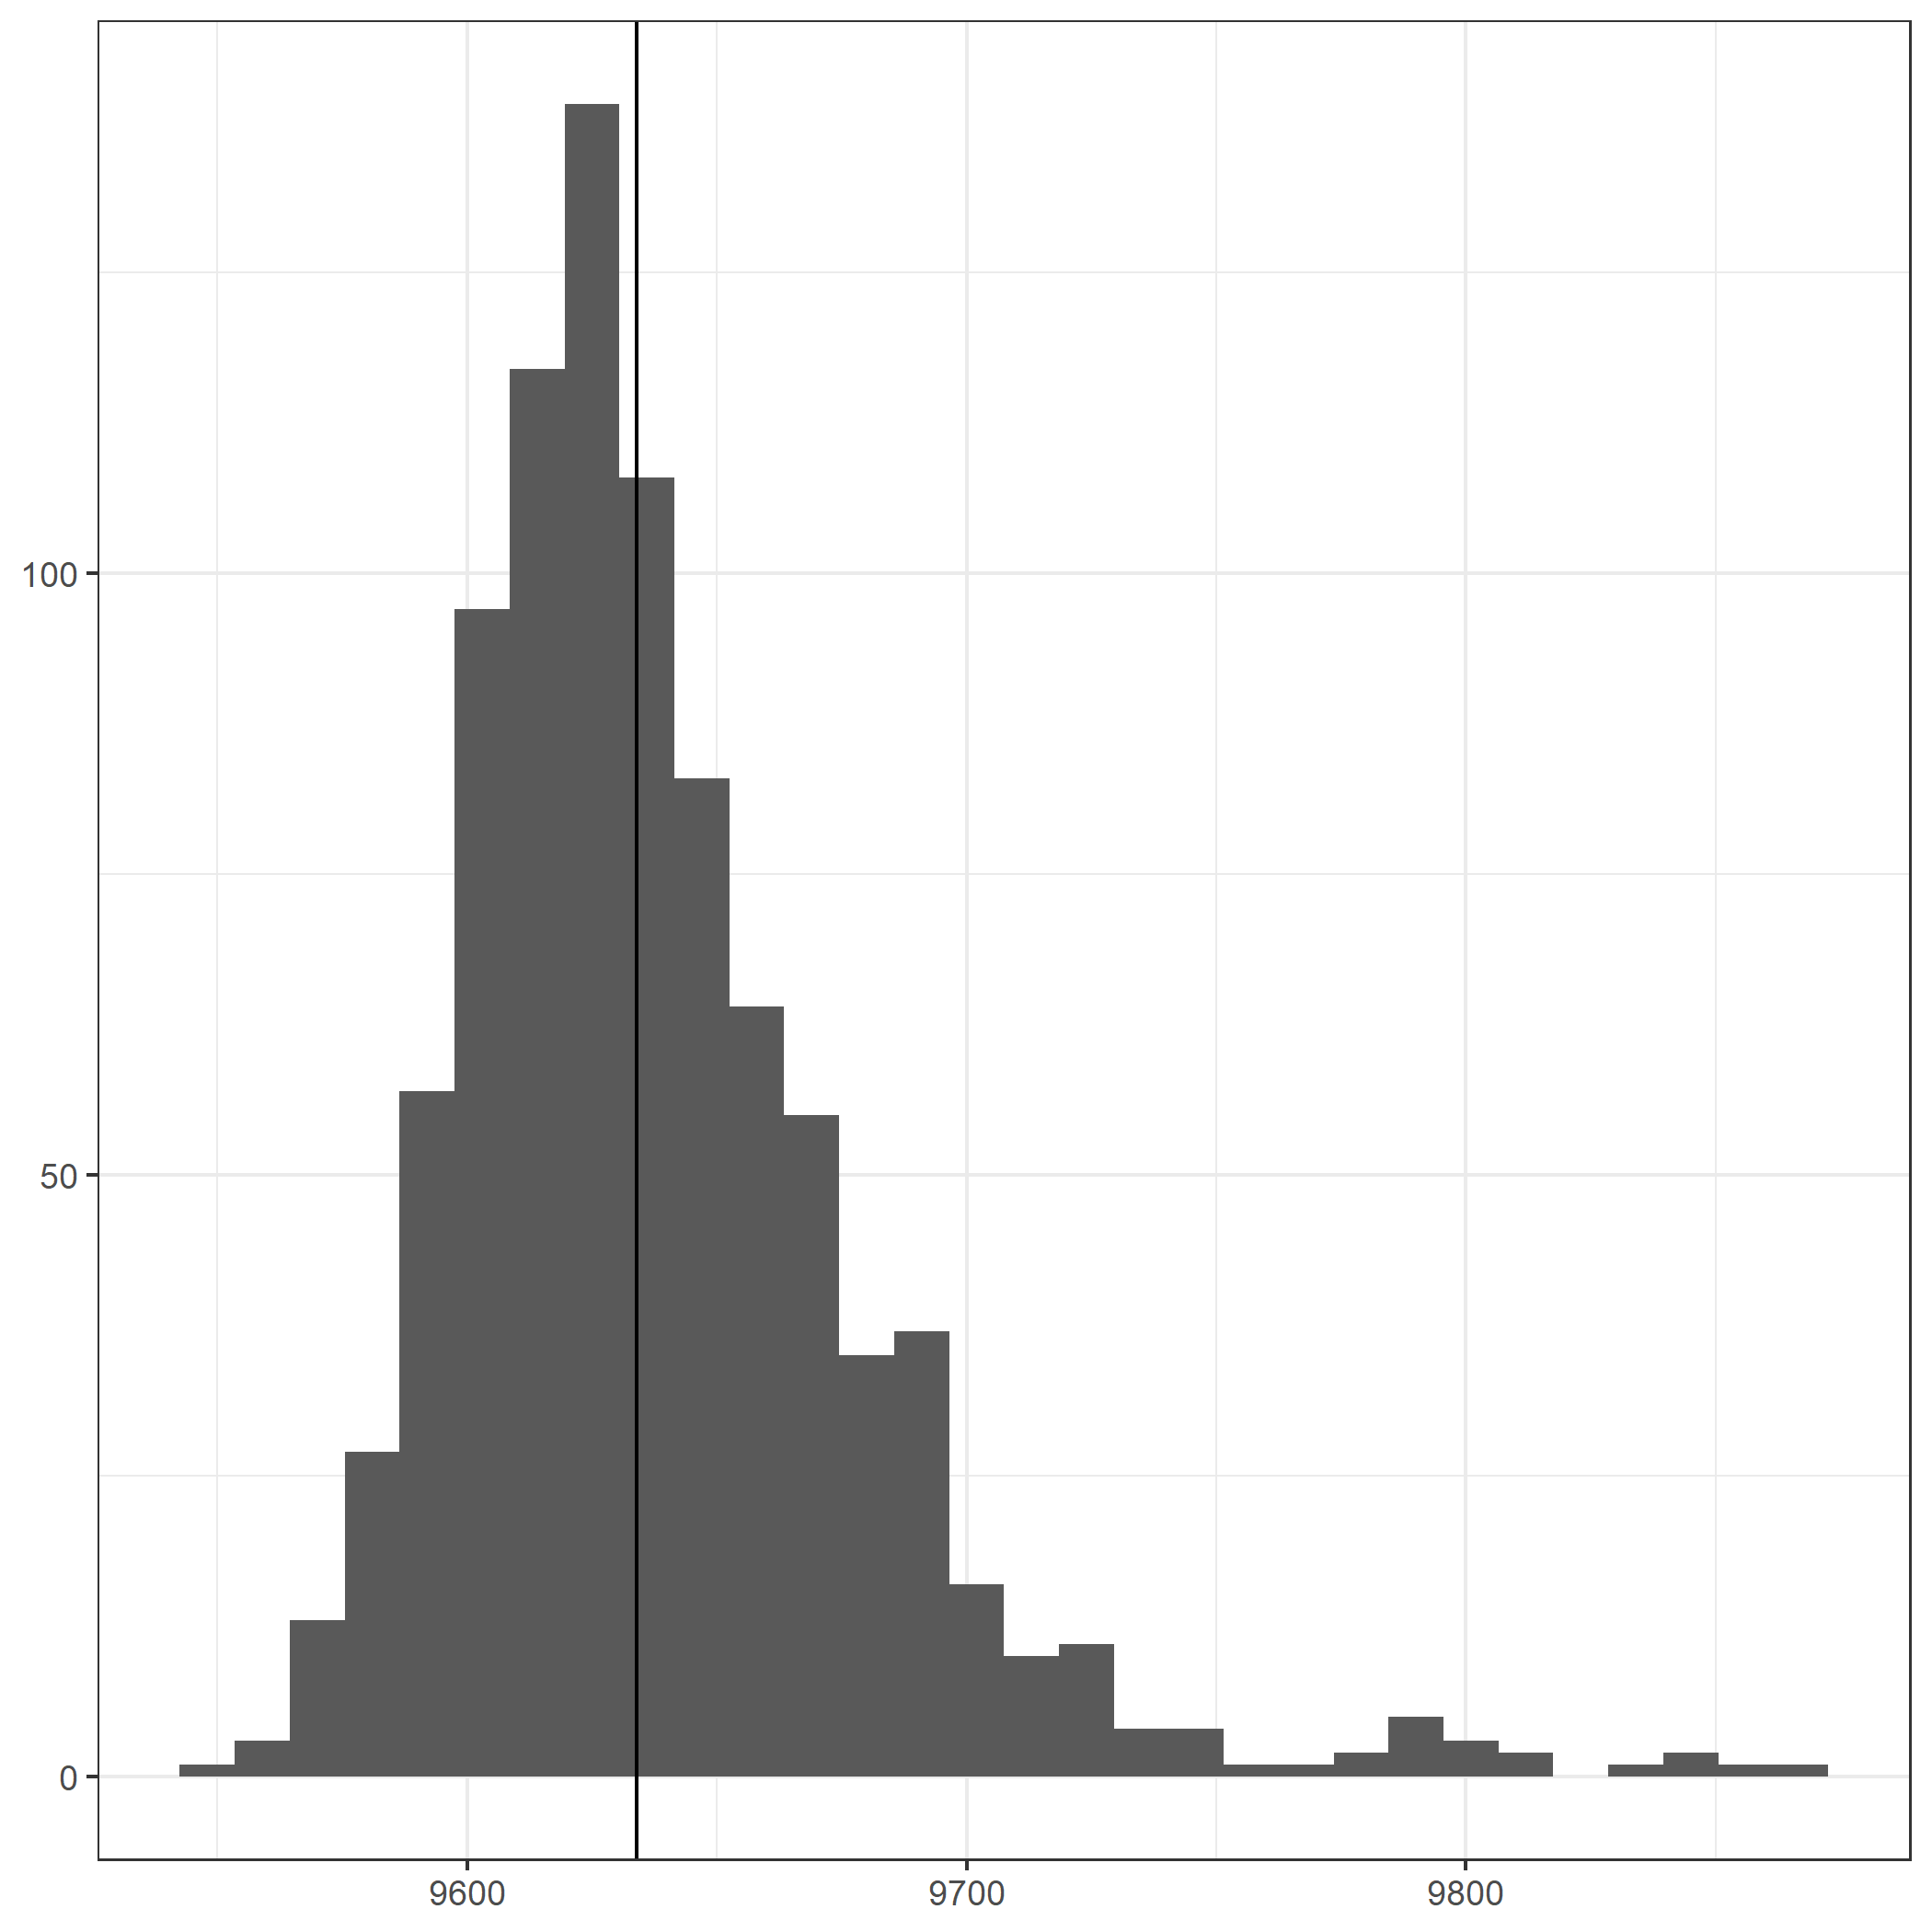
\includegraphics[width=0.6\textwidth]{../notes/figures/nltcs/overlap_posterior4}
			\caption{Posterior distribution and Bayes estimate of overlap across years 1982 and 1989 of NLTCS data.}
			\label{fig:overlap-plot}
		\end{center}
	\end{figure}
	
	%\hypertarget{violations}{%
		%	\subsection{Violations of One-to-One Matching}\label{violations}}
	%
	%As noted previously, the application exhibits many situations in which bipartite matching is difficult. To explore further, we calculate the number of matchings throughout the \texttt{fabl} Gibbs sampler that violate our one-to-one assumption, and find on average 26.17 matchings in violation. These matchings are impossible under the \texttt{BRL} Gibbs sampler, so examining these more closely can provide insight how each model handles situations in which one file in $\bm{X}_1$ has
	%multiple plausible matches in $\bm{X}_2$. 
	%
	%Table~\ref{Tab:rosa-maria} illustrates an example. Note that these records present a near violation of our assumption that there are no duplications within files; we continue to assume that records 825 and 826 in ERTL correspond to different individuals (most likely a mother and daughter), but their records are nearly identical. In addition, using the modified Levenstein distance, the comparison vectors \(\gamma_{2776, 825}\) and \(\gamma_{2776, 826}\) are exactly identical.
	%
	%\begin{table}
	%	\centering
	%	\begin{tabular}[h!]{llllllll}
		%		\hline
		%		Record No. & Dataset & Last Name & First Name & Day & Month & Year & Dept \\
		%		\hline
		%		825 & CDHES & Pineda & Rosa & 6 & 4 & 1984 & NA\\
		%		826 & CDHES & Pineda & Rosa Maria & 6 & 4 & 1984 & NA\\
		%		2776 & ERTL & Pineda & Rosa Maria & 4 & 4 & 1984 & Cuscatlan\\
		%		\hline
		%	\end{tabular}
	%	\caption{Example of linkage situation in which record 2776 in ERTL has multiple plausible matches in CDHES, leading to undesirable behavior both \texttt{fabl} and \texttt{BRL}.}\label{Tab:rosa-maria}
	%\end{table}
	%
	%Figure~\ref{fig:mixing-plot} shows the values that $Z_{825}$ and $Z_{826}$ take on throughout the Gibbs sampler, and demonstrates how each method handles this situation. Under \texttt{fabl}, both records in $\bm{X}_2$ match to the same record in $\bm{X}_1$ throughout the Gibbs process, creating consistent violations of one-to-one matching. Under \texttt{BRL}, the Gibbs process creates one matching configuration and stays there for a while. However, if one pair ``unmatches,'' then the other record has a chance to latch on. Then, the Gibbs process is stuck with that matching status for a while, resulting in a Gibbs process with poor mixing. 
	%
	%Through its independent sampling,\texttt{fabl} allows the modeler to inspect records with multiple plausible matches, and if they desire, to then choose the record pairing with the highest posterior probability. \texttt{BRL} in contrast, in strictly enforcing one-to-one matching throughout the sampler, can lead to situations where none of the plausible matches reach the threshold to be identified through the Bayes estimate. Thus relaxing the one-to-one constraint has served as a useful tool for identifying model misspecification. 
	%
	%\begin{figure}[h!]
	%\begin{center}
	%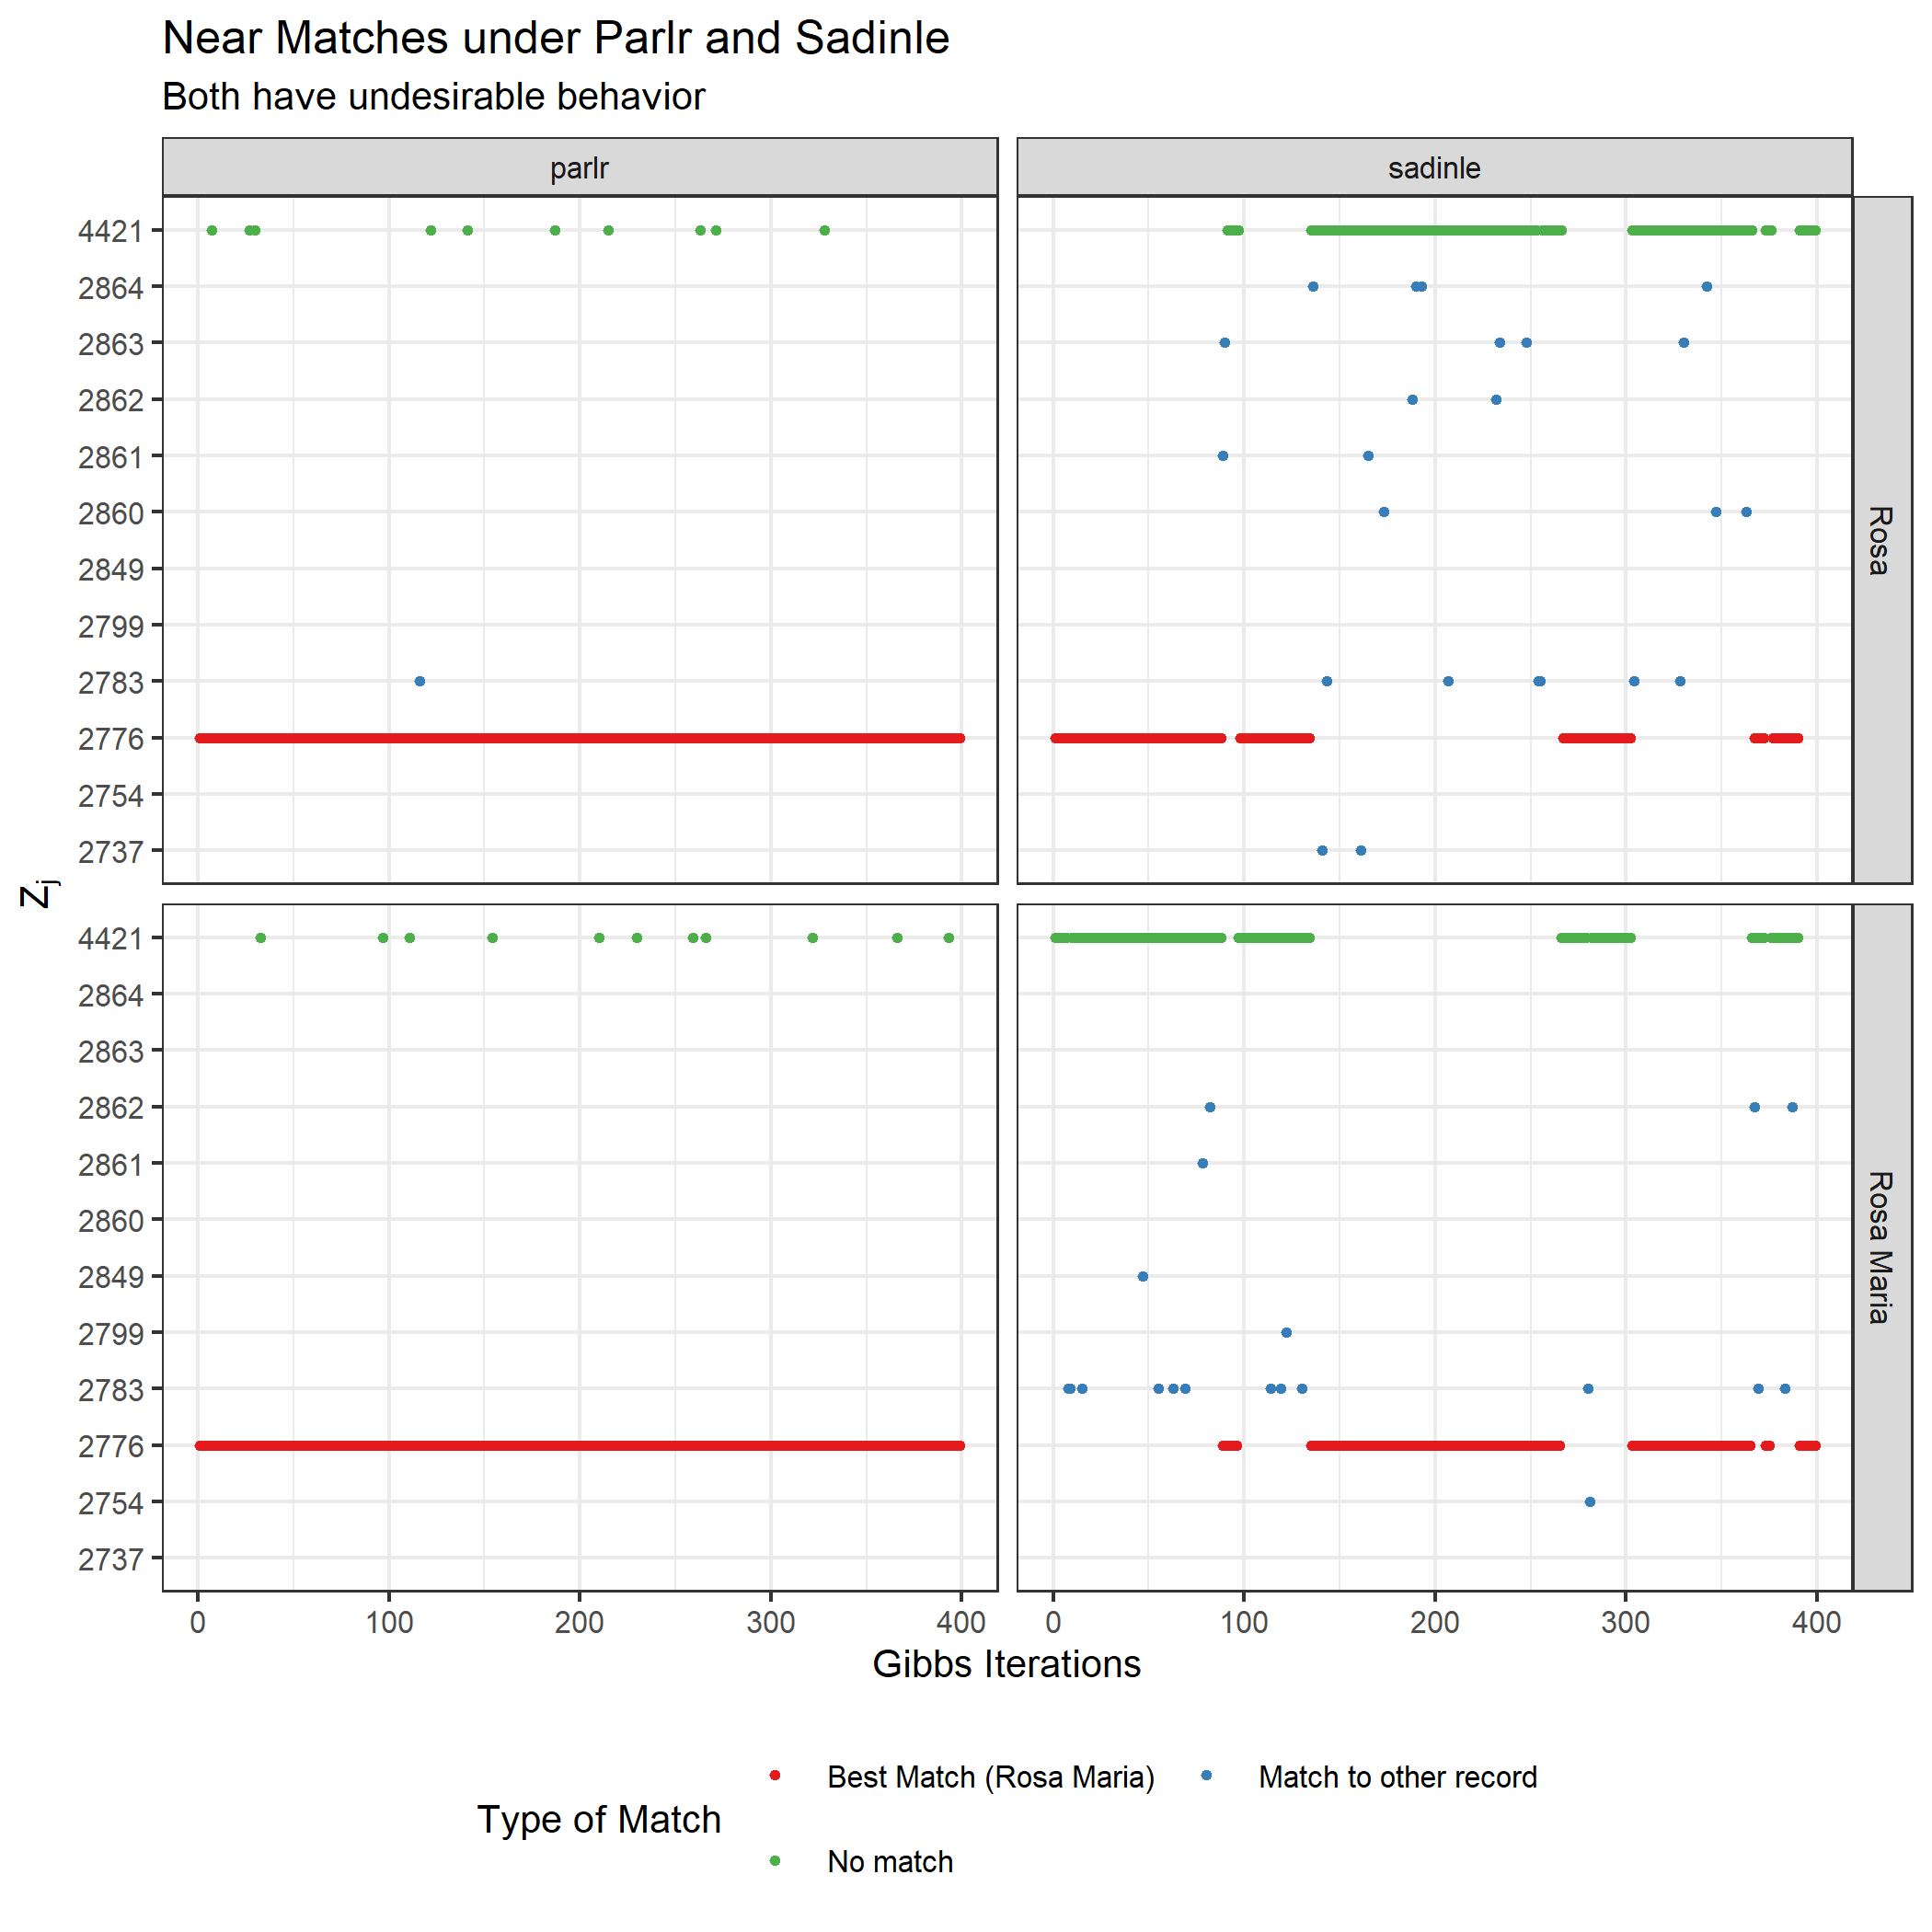
\includegraphics[width=0.6\textwidth]{../notes/figures/el_salvador/bad_mixing} 
	%\caption{Gibbs sampling in situation with multiple plausible matches. Under \texttt{BRL}, two records in ERTL compete for their most similar record, splitting the posterior probability. Under \texttt{fabl}, both record consistently match with their most similar record, consistently violating one-to-one matching.} \label{fig:mixing-plot}
	%\end{center}
	%\end{figure}
	
	\section{Conclusion}
	\label{discussion}
	
	In this paper, we have proposed \texttt{fabl}, a Bayesian record linkage method that scales to large data sets. We have proven that the proposed hashing method
	and model assumptions allow for a linkage procedure whose computational complexity does not scale with the size of the larger dataset. This makes \texttt{fabl} computationally advantageous in many linkage scenarios, particularly when one datafile is substantially smaller than the other. We have demonstrated the speed and accuracy of \texttt{fabl} by replicating a simulation study and a case study in \cite{sadinle_bayesian_2017}, and through an additional case study that is computationally infeasible under \texttt{BRL}. Open source software to use \texttt{fabl} in \texttt{R} is available through \href{https://github.com/briankundinger/parlrdev}{Github}.
	
	%Throughout our paper, we have discussed independent pairwise matching assumptions, one-to-one matching assumptions, and when such assumptions are not met in practice. We explored ``one-to-many'' scenarios in which one record in $\bm{X}_2$ has multiple plausible matches in $\bm{X}_1$, and showed how both \texttt{fabl} and \texttt{BRL} demonstrated undesirable qualities. Other issues arise under ``many-to-one'' scenarios, where one record in $\bm{X}_2$ has multiple plausible matches in $\bm{X}_1$, and ``many-to-many'' scenarios in which there is duplication both across and within datasets. Extending \texttt{fabl} in such scenarios with a more robust linkage structure parameter $\bm{Z}$ is a topic for future work. 
	%
	%To our knowledge, \texttt{fabl} is the first method within the Fellegi Sunter comparison vector approaches with an interpretable parameter for the rate of matching across datasets. This motivates extensions to \texttt{fabl} with additional parameters that allow the quality of information (the $\bm{m}$ and $\bm{u}$ parameters) and the rate of matching (the $\lambda$ parameter) to differ by subgroups in the linkage task. Similar work has been been proposed by \cite{wortman2019} and \cite{Larsen2005}, and would need to be adapted for our prior distribution and model assumptions. We see these types of heirarchical record linkage models as potential contributions to the growing algorithmic fairness literature, and useful to practitioners working with or studying marginalized populations. 
	
	%Tuning \texttt{fabl} for use in these scenarios is one potential avenue for
	%future work.
	
	%\begin{figure}[t]
	%	
	%	{\centering 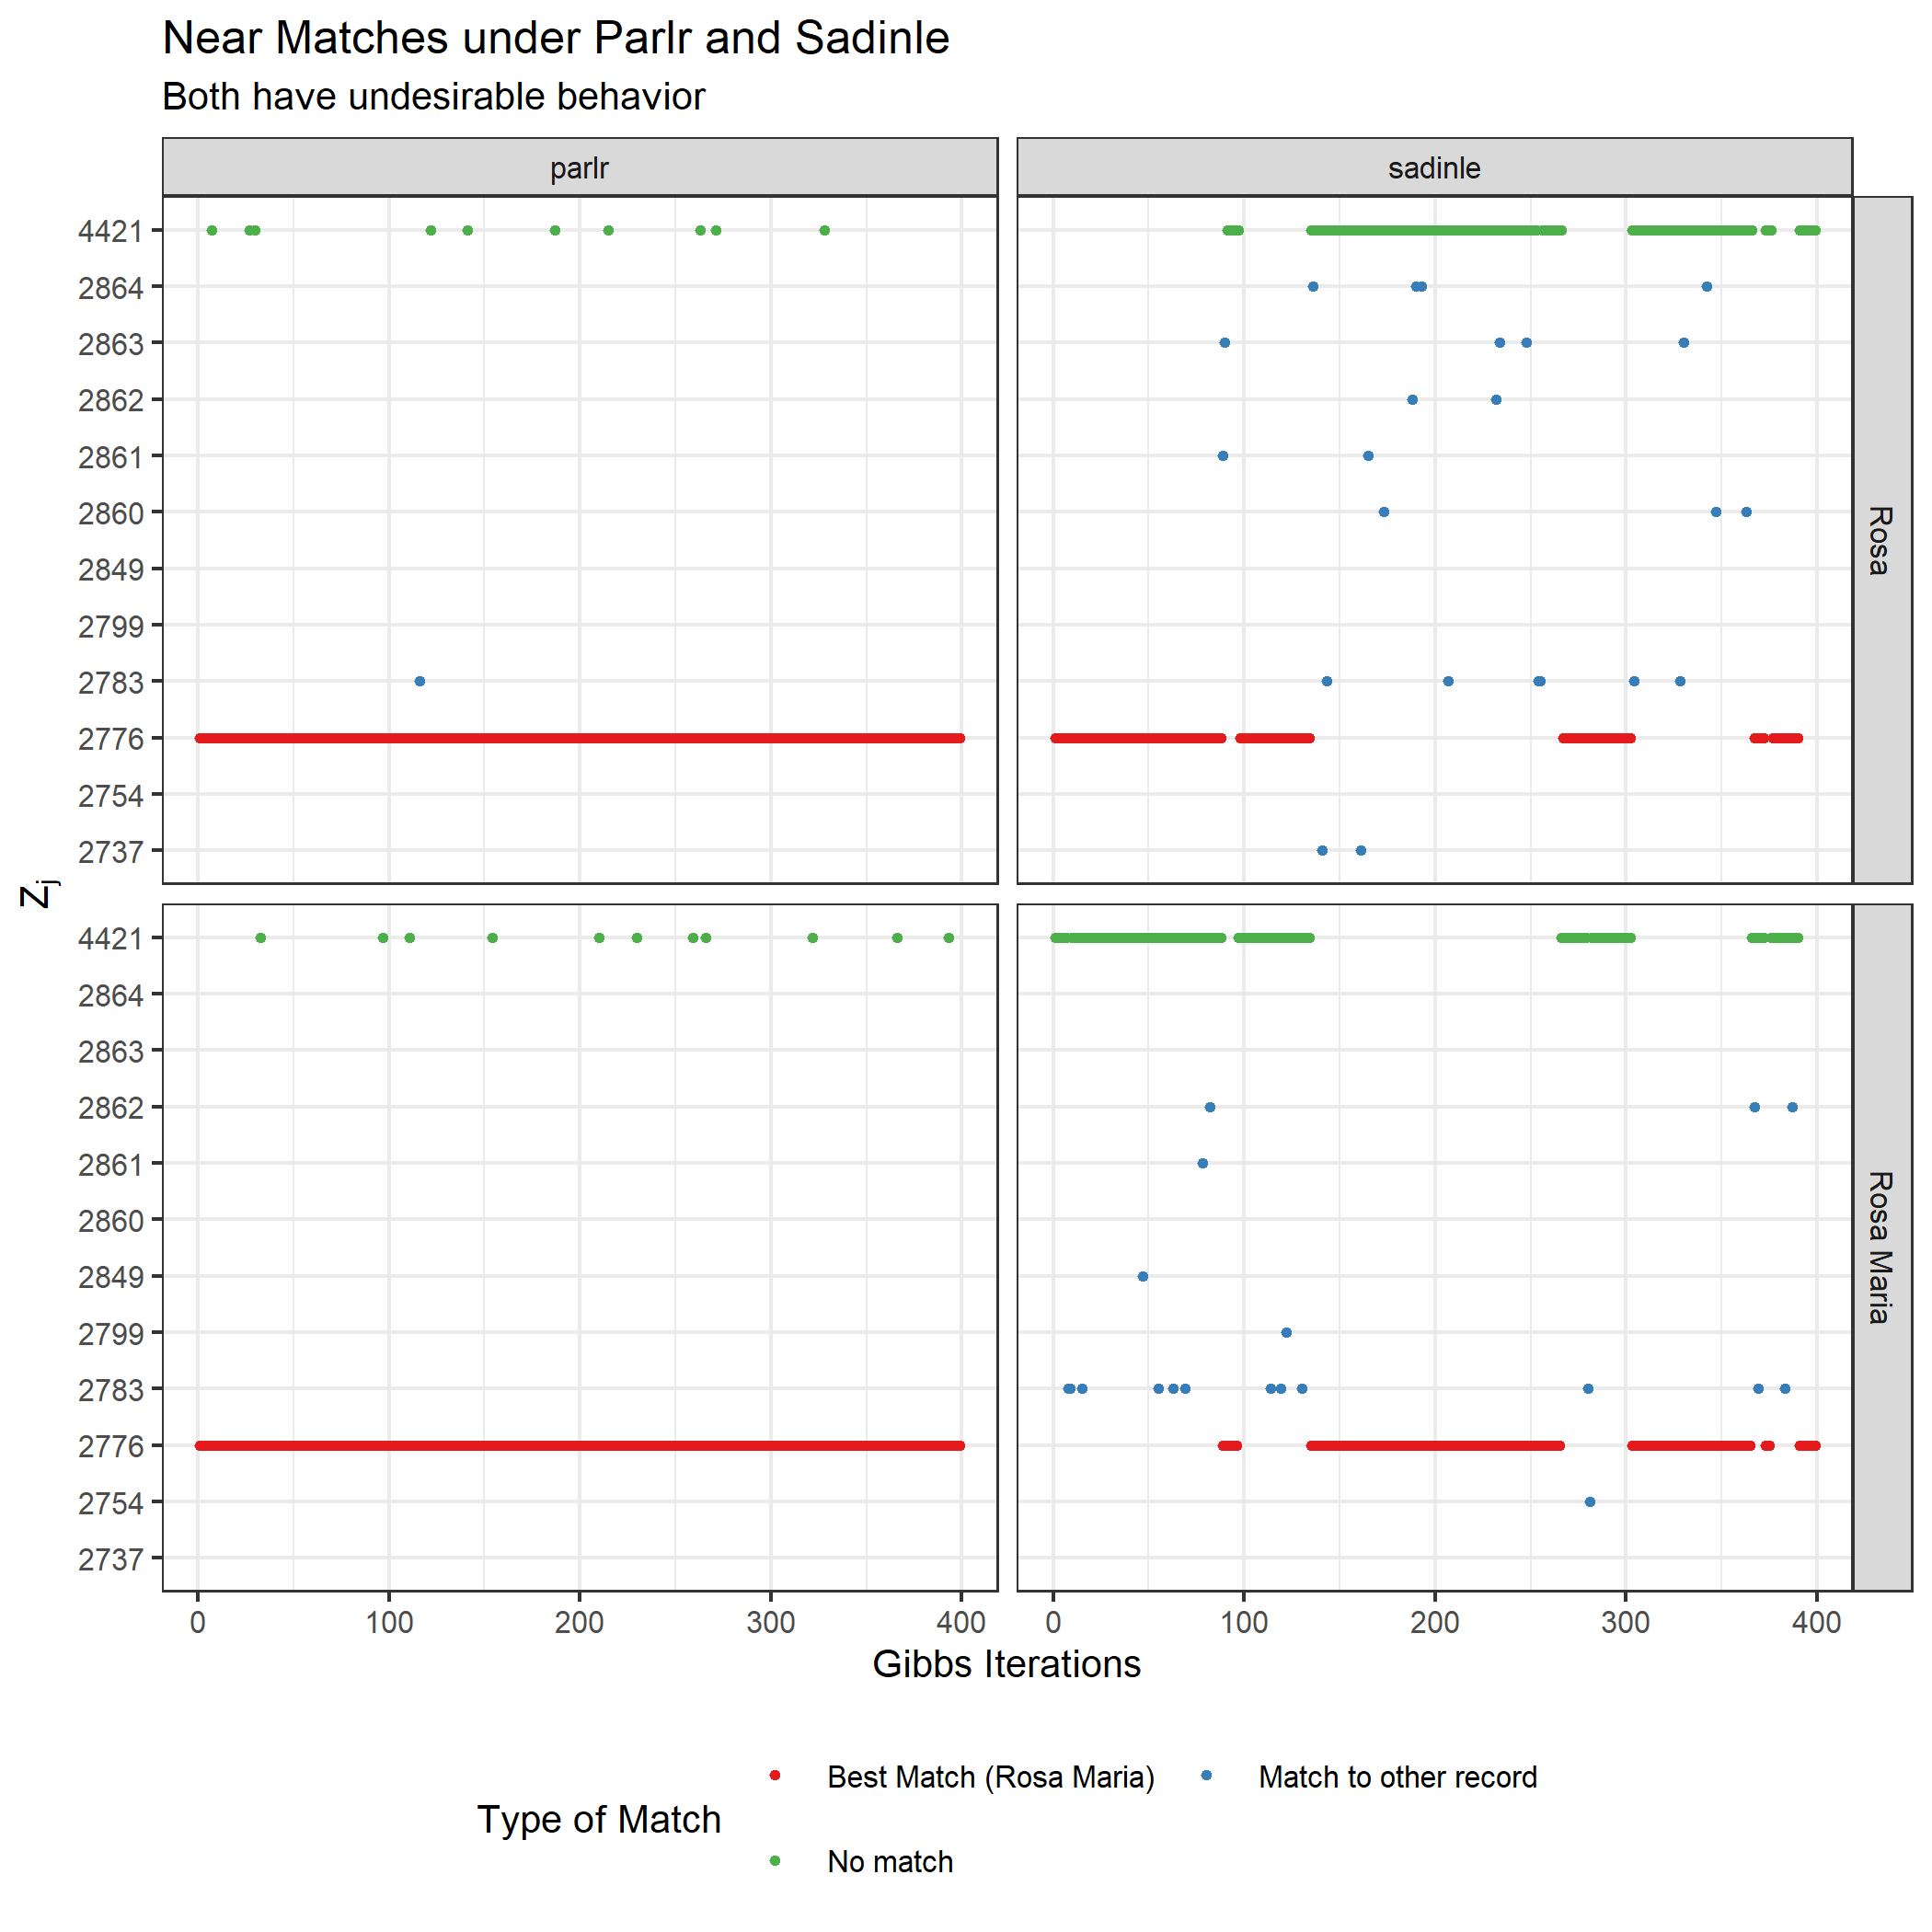
\includegraphics[width=0.6\textwidth]{../notes/figures/el_salvador/bad_mixing} 
		%		
		%	}
	%	
	%	\caption{Gibbs sampling in situation with multiple plausible matches.}\label{fig:mixing-plot}
	%\end{figure}
	
	%\subsection{National Long Term Care Survey}
	%\label{nltcs} 
	%
	%The National Long Term Care Survey is a longitudinal study to track changes in health among Medicare recipients. It was conducted approximately every five years, and we concern ourselves here with linking records from years 1982 and 1989. The data only contains day, month, and year of birth, sex, state the individual lives in, and regional office. State and regional office have been anonymized, presented as numbers instead of their actual values. We construct the comparison vectors using only binary exact matching for each field, since there is no straightfoward way to incorporate partial matching in this context. The 1982 file contains $n_A = 20485$ records, 1989 file contains $n_B = 17466$ files, and the six linkage fields induces $2^6 = 64$ possible unique agreement patterns. We note that linkage quality is bound to be quite weak for many potential matches with such a large number of records and such limited identifying information.  
	%
	%With such large files, performing all-to-all comparisons under the original Fellegi-Sunter framework is infeasible. Indeed, this would require nearly 400 million comparison vectors, each containing 6 integer comparisons; the resulting data object would contain over 2 billion integers, and would require approximately 16 GBs of memory to hold. Instead, we take the partitioning approach reviewed in \ref{data-representation-hashing-and-storage}, and split each dataset into 10 smaller datasets. We use parallel computing on cluster service create the comparison vectors for each pair of data chunks, hash the results, and compress in size through storage efficient indexing. We then aggregate the results, creating a data object of just 87 MB, and proceed with the Gibbs Sampler. 
	%
	%Were a personal computer able to hold the 16 GB data object required by the direct approach, the Gibbs sampler under \texttt{BRL} would be tortuously slow, with computational complexity $O(n_A \times n_B \times F)$ where $n_A = 20485$. However, under \texttt{fabl} the sampler has complexity $O(P \times n_B \times F)$ where $P = 64$, so 1000 iterations of the Gibbs sampler are completed in just XX seconds. Posterior analysis yields an initial estimate of 9991 individuals linked across the the two datasets, and 8895 individuals linked once conflicts are resolved to ensure one-to-one matching. 
	%
	%Lastly, we comment on the significance of conducting this linkage without the use of deterministic blocking. With previous methods, one could link these two records by blocking on a certain field, and running separate Gibbs samplers on each of the separate blocks. This strategy drastically improves computation since it significantly reduces the number of comparison vectors that need to be formed and uses smaller data objects throughout the sampler. However, this computational savings comes at the cost of missing potential links, specifically in cases where the blocking variable is recorded in error. In this case, 62 of the matched pairs exhibit a disagreement in sex, 17 exhibit a disagreement in state, and 39 exhibit a disagreement in regional office. We have no way to verify that the matches found under \texttt{fabl} are indeed correct, so it is possible that matches found with such disagreements are false positives. Even if not, the modeler may conclude that, for example, 17 missed matches are a small price to pay to be able to block on state and run 50 smaller, independent linkage procedures. However, \texttt{fabl} allows the modeler to make this choice for themselves, rather than being forced to do so for computational reasons. Additionally, by running on the Gibbs sampler the entirety of both files, we achieve $m$ and $u$ parameters that are interpretale for the entire study, rather than separate parameters for each block. Although these $m$ and $u$'s are often regarded as nuisance parameters in the record linkage literature, \texttt{fabl} allows for study of these parameters that has been been possible before. 
	
	\clearpage
	
	\bigskip
	
	\bibliographystyle{jasa}
	\bibliography{biblio}
	
	\clearpage
	
	\section*{Appendix}
	\label{sec:appendix}
	
	
	
	\hypertarget{app:fabl-psuedocode}{%
		\subsection{Summary of Fast Beta Linkage Method}\label{app:fabl-psuedocode}}
	
	\begin{algorithm}[h!]
		\begin{algorithmic}[1]
			
			\Procedure{Hashing and Preprocessing}{}
			\State Construct and enumerate set of unique patterns $\mathcal{P}$ from $F$ and $\{L_f\}$.
			\State Partition files $\bm{X_1}$ and $\bm{X_1}$ into chunks $\{\bm{X_{1n}}\}$, $\{\bm{X_{2m}}\}$.
			\For{each $n$, $m$}
			\State Create comparison vectors between $\bm{X_{1n}}$ and $\bm{X_{2m}}$.
			\State Hash records to $\mathcal{R}_{nm}$ and calculate summary statistics $\mathcal{H}_{nm}$.
			\State Use SEI to reduce memory usage; $\mathcal{R}_{nm} \to \mathcal{R}_{nm}^{\text{SEI}}$.
			\EndFor
			\State Synthesize results across pairings to get $\tilde{\Gamma} = \{\mathcal{P}, \mathcal{R}, \mathcal{H} \}$.
			\EndProcedure
			
			\Procedure{Gibbs Sampling}{}
			\State Initialize $m$, $u$, and $Z$ parameters.
			
			\For{$t \in \{1, \ldots, T\}$} 
			\State Sample $\Phi^{t+1}|Z^{t}, \tilde{\Gamma}$.
			\State Sample $h\left(Z^{t+1}\right)|\Phi^{t+1}, \tilde{\Gamma}$.  \Comment{Sample agreement pattern, not record}
			\EndFor
			\State Sample $Z | h(Z), \tilde{\Gamma}$. \Comment{Fills in record label based on agreement pattern}
			
			\EndProcedure
			
		\end{algorithmic}
	\end{algorithm}
	\clearpage
	
	\hypertarget{app:ohe}{%
		\subsection{One Hot Encoding Transformation}\label{app:ohe}}
	
	\texttt{fabl} makes use of one-hot encodings to aid in vectorized computations. For $\gamma_{ij}^f$ with $L_f$ levels, define $e_{ij}^f$ to be an $L_f \times 1$ vector.  When $\gamma_{ij}^f = \ell$, we set the $\ell^{th}$ element of $e_{ij}^f$ to be 1, and set the other $L_f - 1$ elements of $e_{ij}^f$ to be 0. We then concatenate the $e_{ij}^f$ for all $f \in \{1, \ldots, F\}$, resulting in the one-hot encoded comparison vector $e_{ij}$ of length $\sum_{f=1}^F L_f$.
	
	For example, consider comparing the toy records shown in Table \ref{tab:ohe} with $L = (3, 3, 2, 2)$ levels of agreement for last name, first name, DOB, and city respectively. Since the first name differs by only one letter, a reasonable comparison vector for this pair would be $\gamma_{ij} = (1, 2, 1, 2)$. The one hot encoding representation of this vector is $e_{ij} = (1, 0, 0, 0, 1, 0, 1, 0, 0, 1)$. 
	\begin{table}[h!]
		\centering
		\begin{tabular}[h!]{llll}
			\hline
			Last Name & First Name & DOB & City \\
			\hline
			Smith & Taylor & 01/01/2000 & Durham\\
			Smith & Tayler & 01/01/2000 & Raleigh\\
			\hline
		\end{tabular}
		\caption{Example records for one hot encoding.}\label{tab:ohe}
	\end{table}
	
	
	\hypertarget{appendix-sim}{%
		\subsection{Traceplots for Simulation Study}\label{app:appendix-sim}}
	Below are traceplots for one of the 900 linkage tasks that comprise the simulation in Section \ref{accuracy}. It is set up with one error across the linkage fields and 50 duplicates across files. Traceplots across other settings exhibit similar behavior. Note that traceplots for $\bf{u}$ parameters show very little variation because the overwhelming majority of record pairs are nonmatching.  
	
	\begin{figure}[!h]
		\begin{center}
			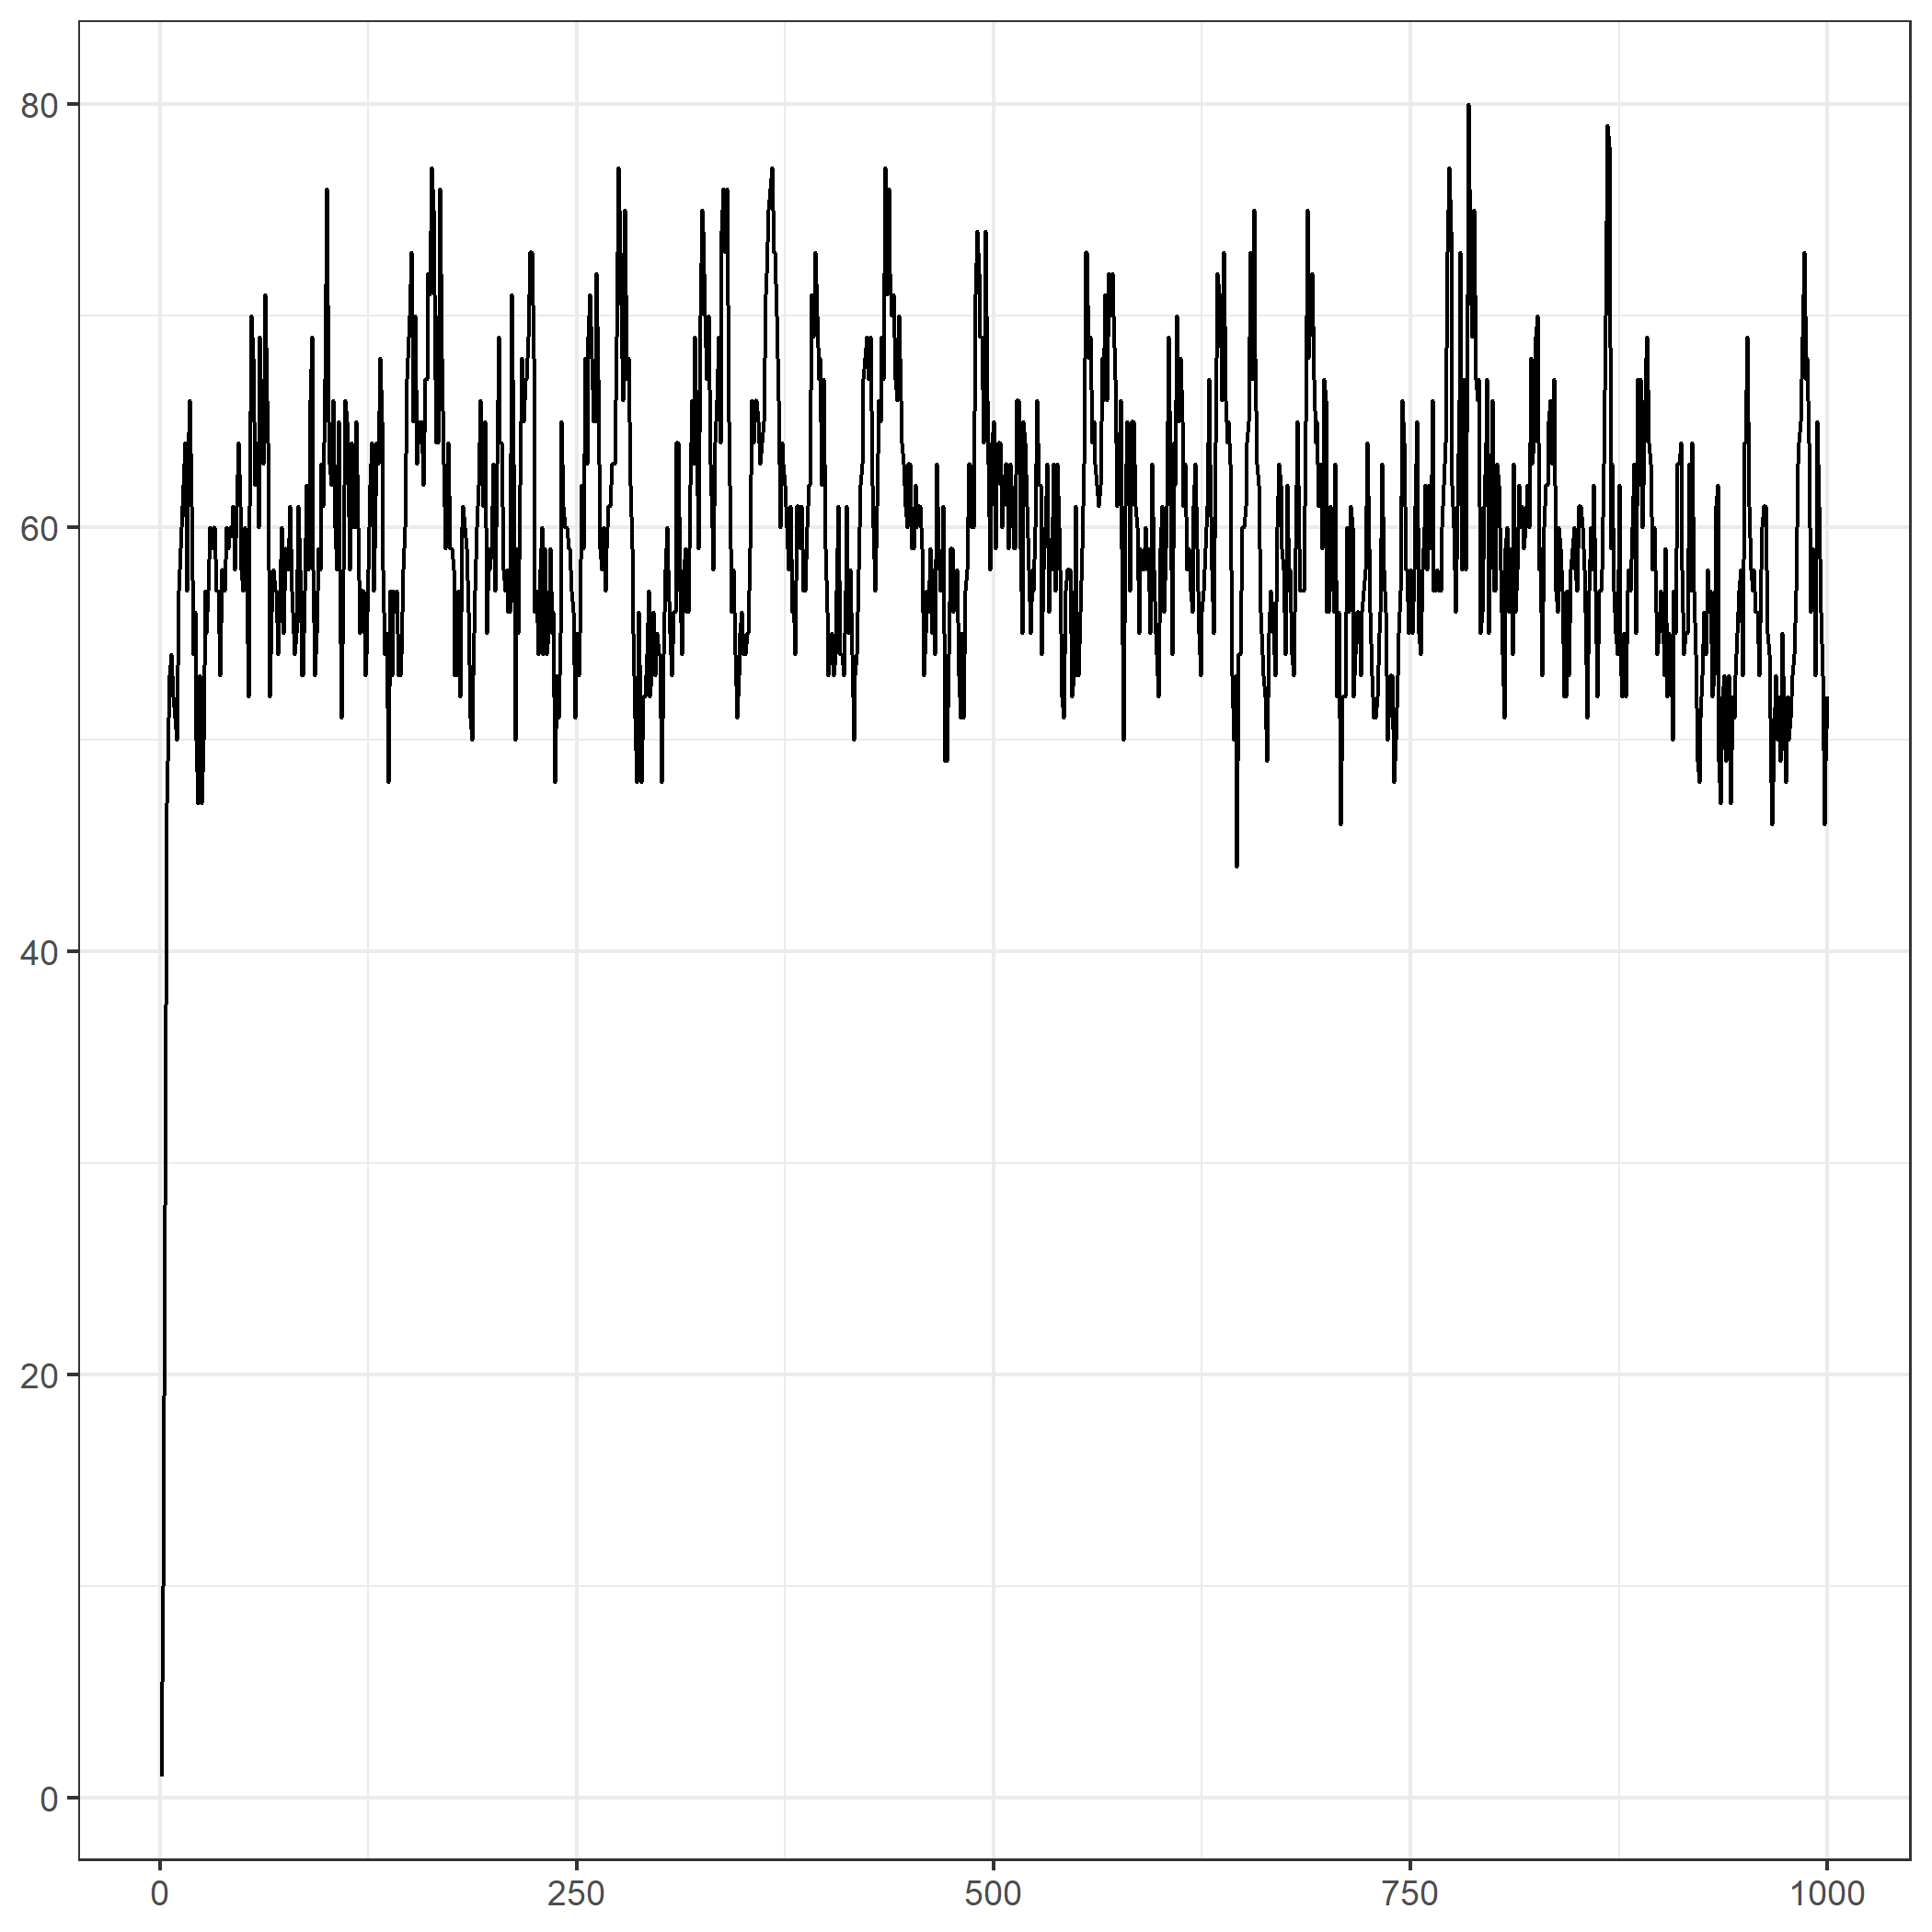
\includegraphics[width=0.6\textwidth]{../notes/figures/sim_overlap_trace} 
			\caption{Representative traceplot of overlap between files from simulation study in Section \ref{accuracy}}\label{fig:sim_overlap_trace}
		\end{center}
	\end{figure}
	
	
	
	\begin{figure}[!h]
		\begin{center}
			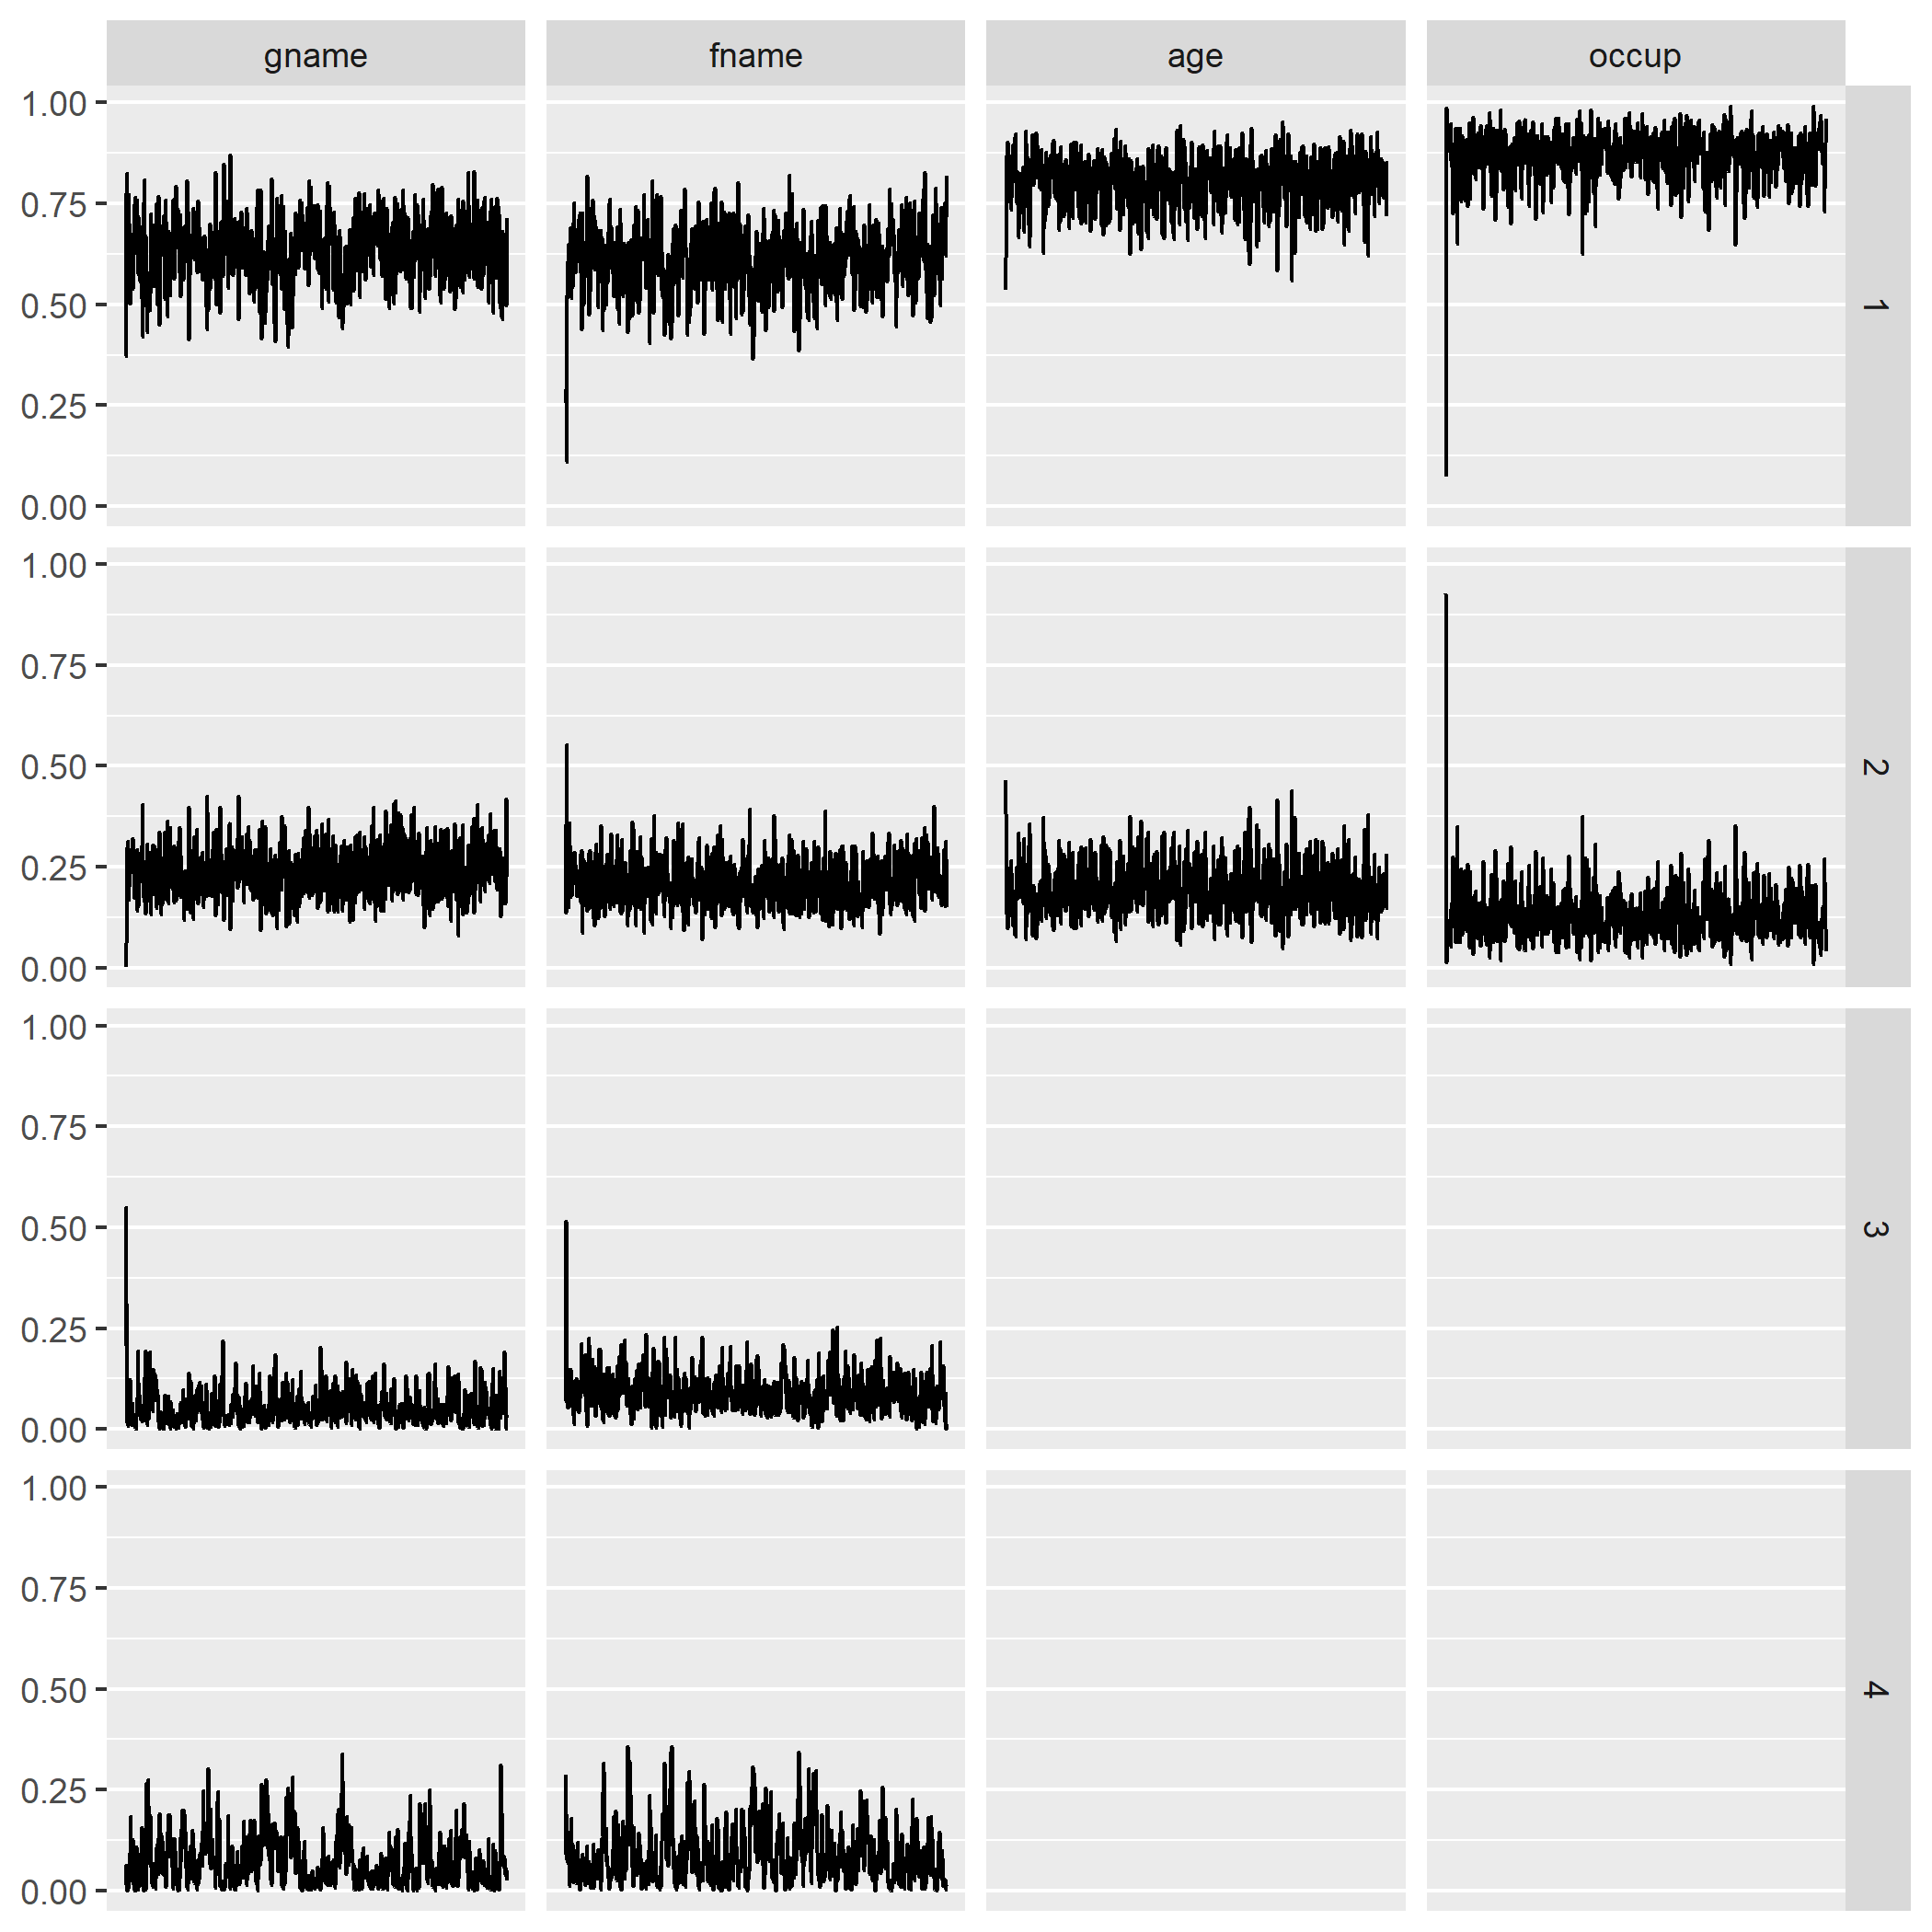
\includegraphics[width=0.6\textwidth]{../notes/figures/sim_m_trace} 
			\caption{Representative traceplot of m parameter from simulation study in Section \ref{accuracy}}\label{fig:sim_m_trace}
		\end{center}
	\end{figure}
	
	\begin{figure}[!h]
		\begin{center}
			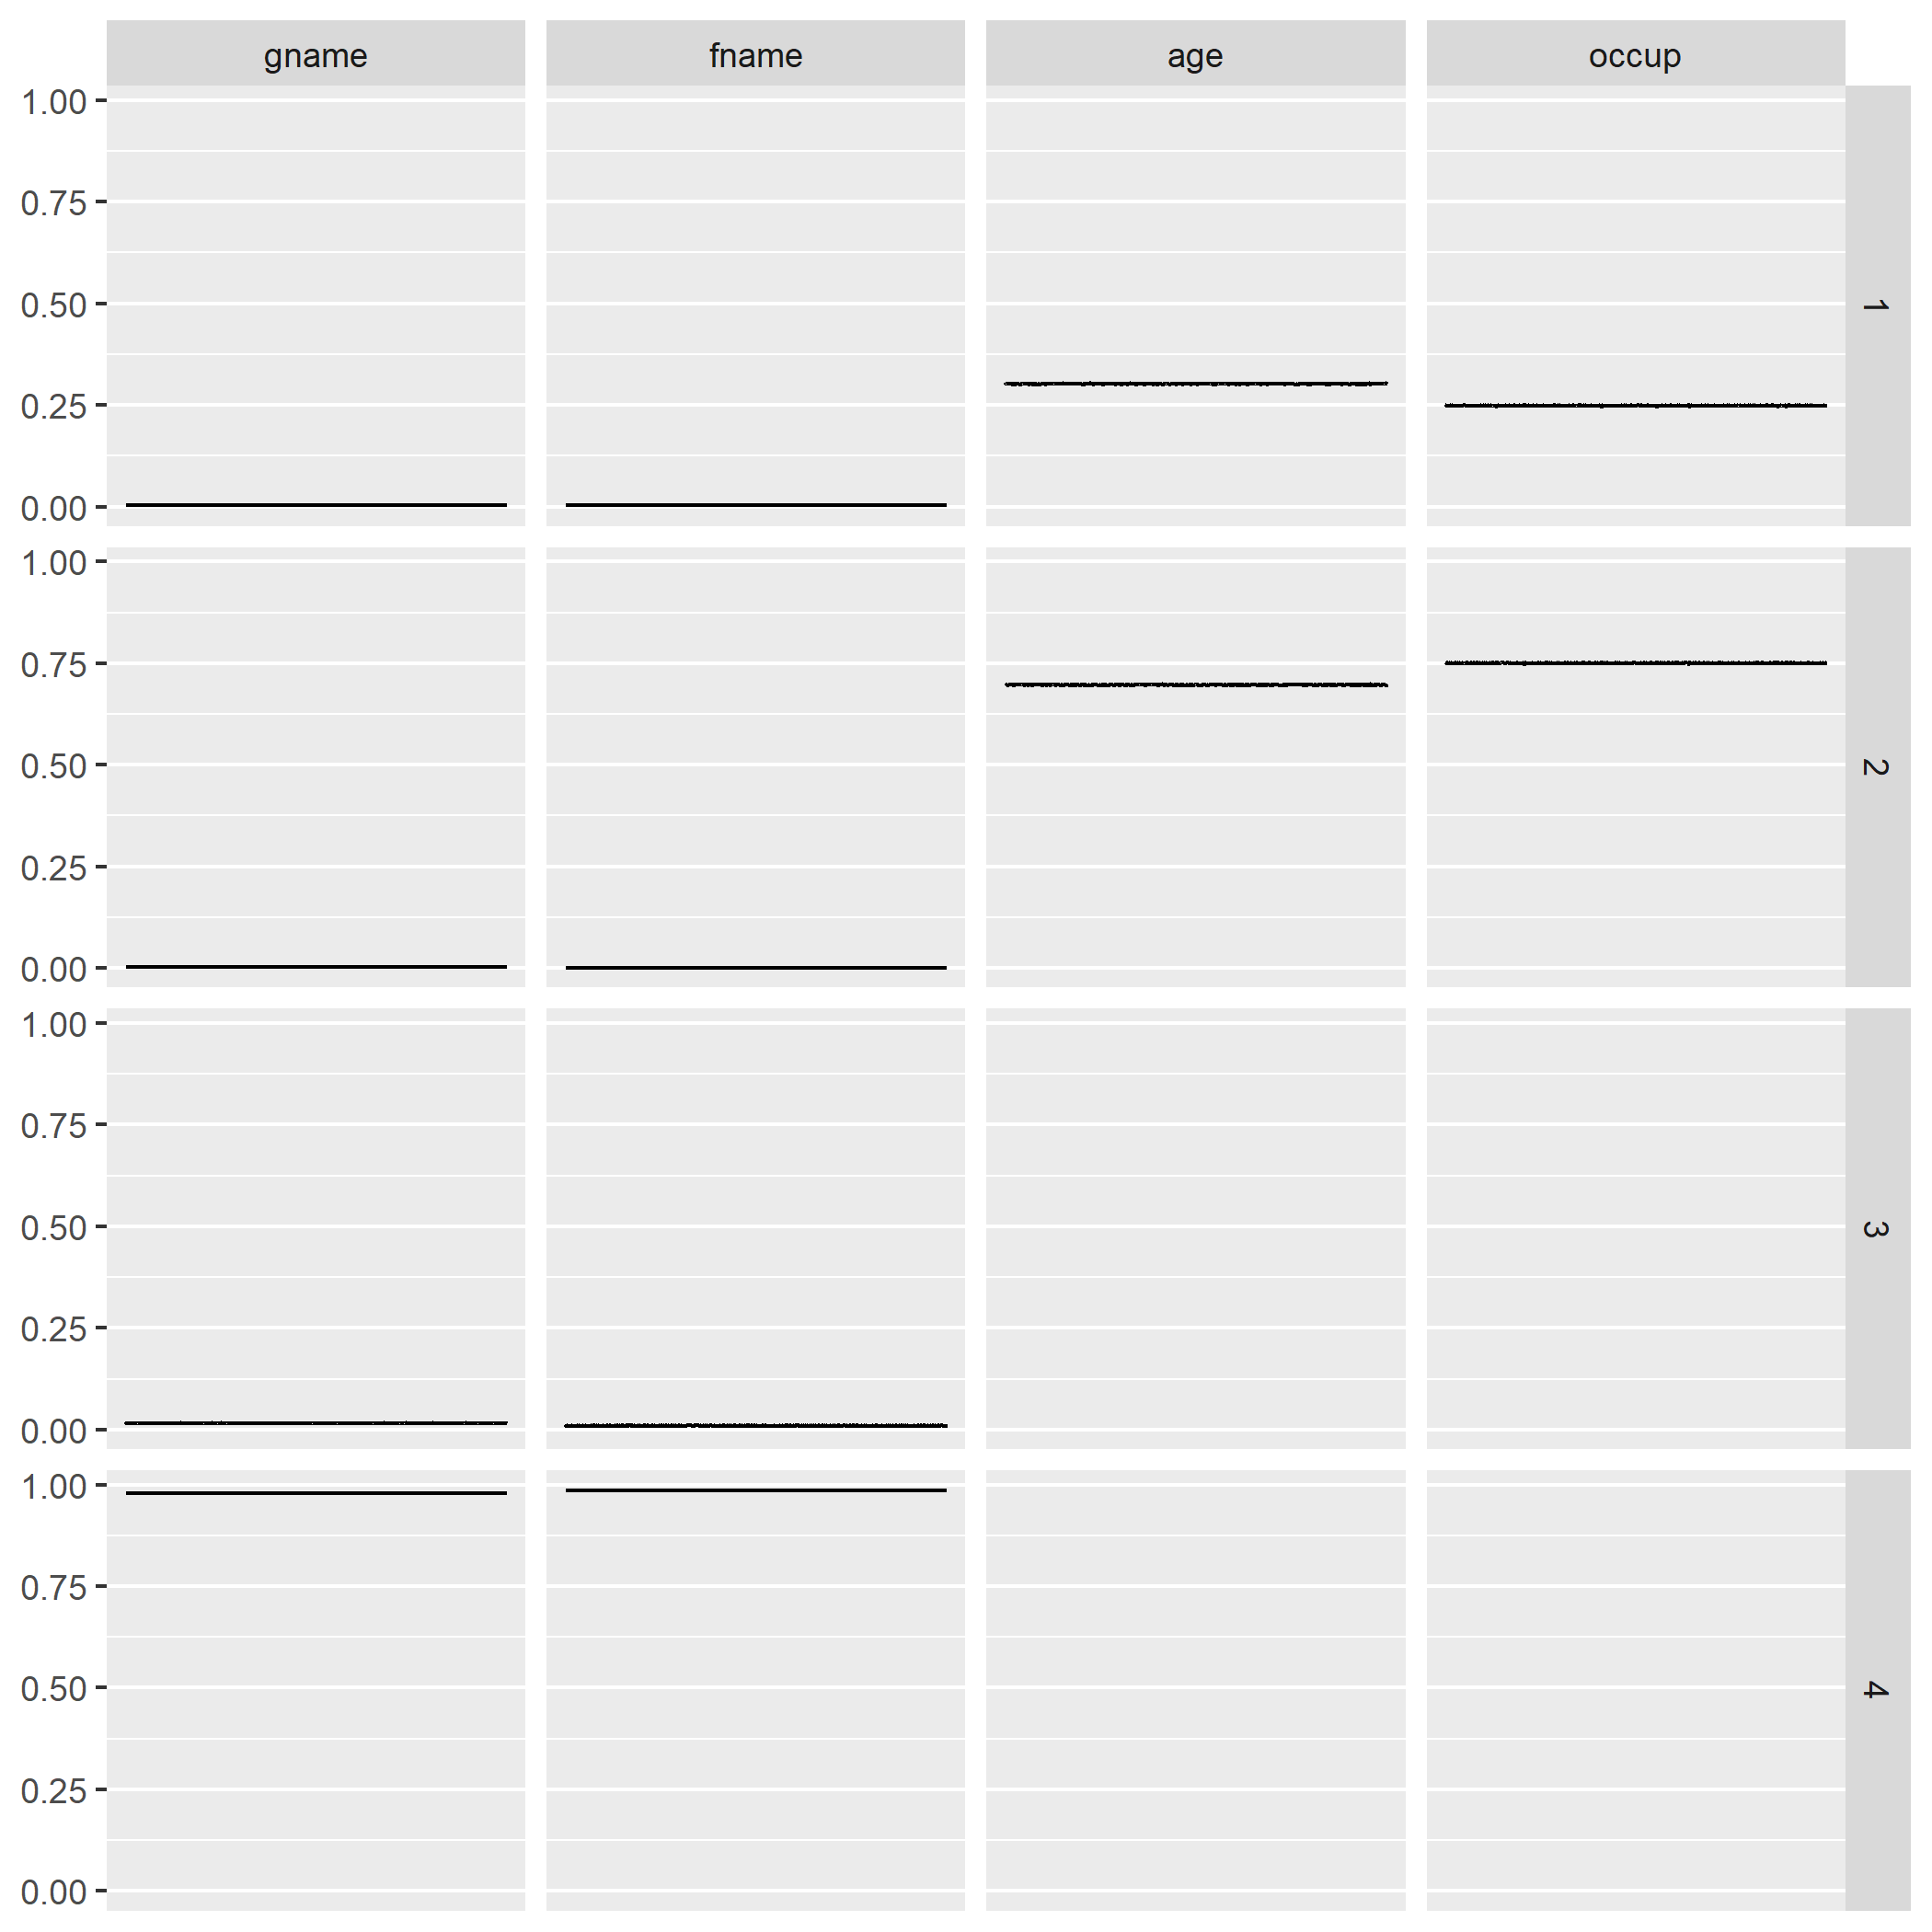
\includegraphics[width=0.6\textwidth]{../notes/figures/sim_u_trace} 
			\caption{Representative traceplot of u parameters from simulation study in Section \ref{accuracy}}\label{fig:sim_u_trace}
		\end{center}
	\end{figure}
	
	\clearpage
	
	\hypertarget{appendix-es}{%
		\subsection{Traceplots for El Salvador Case Study}\label{app:appendix-es}}
	
	\begin{figure}[!h]
		\begin{center}
			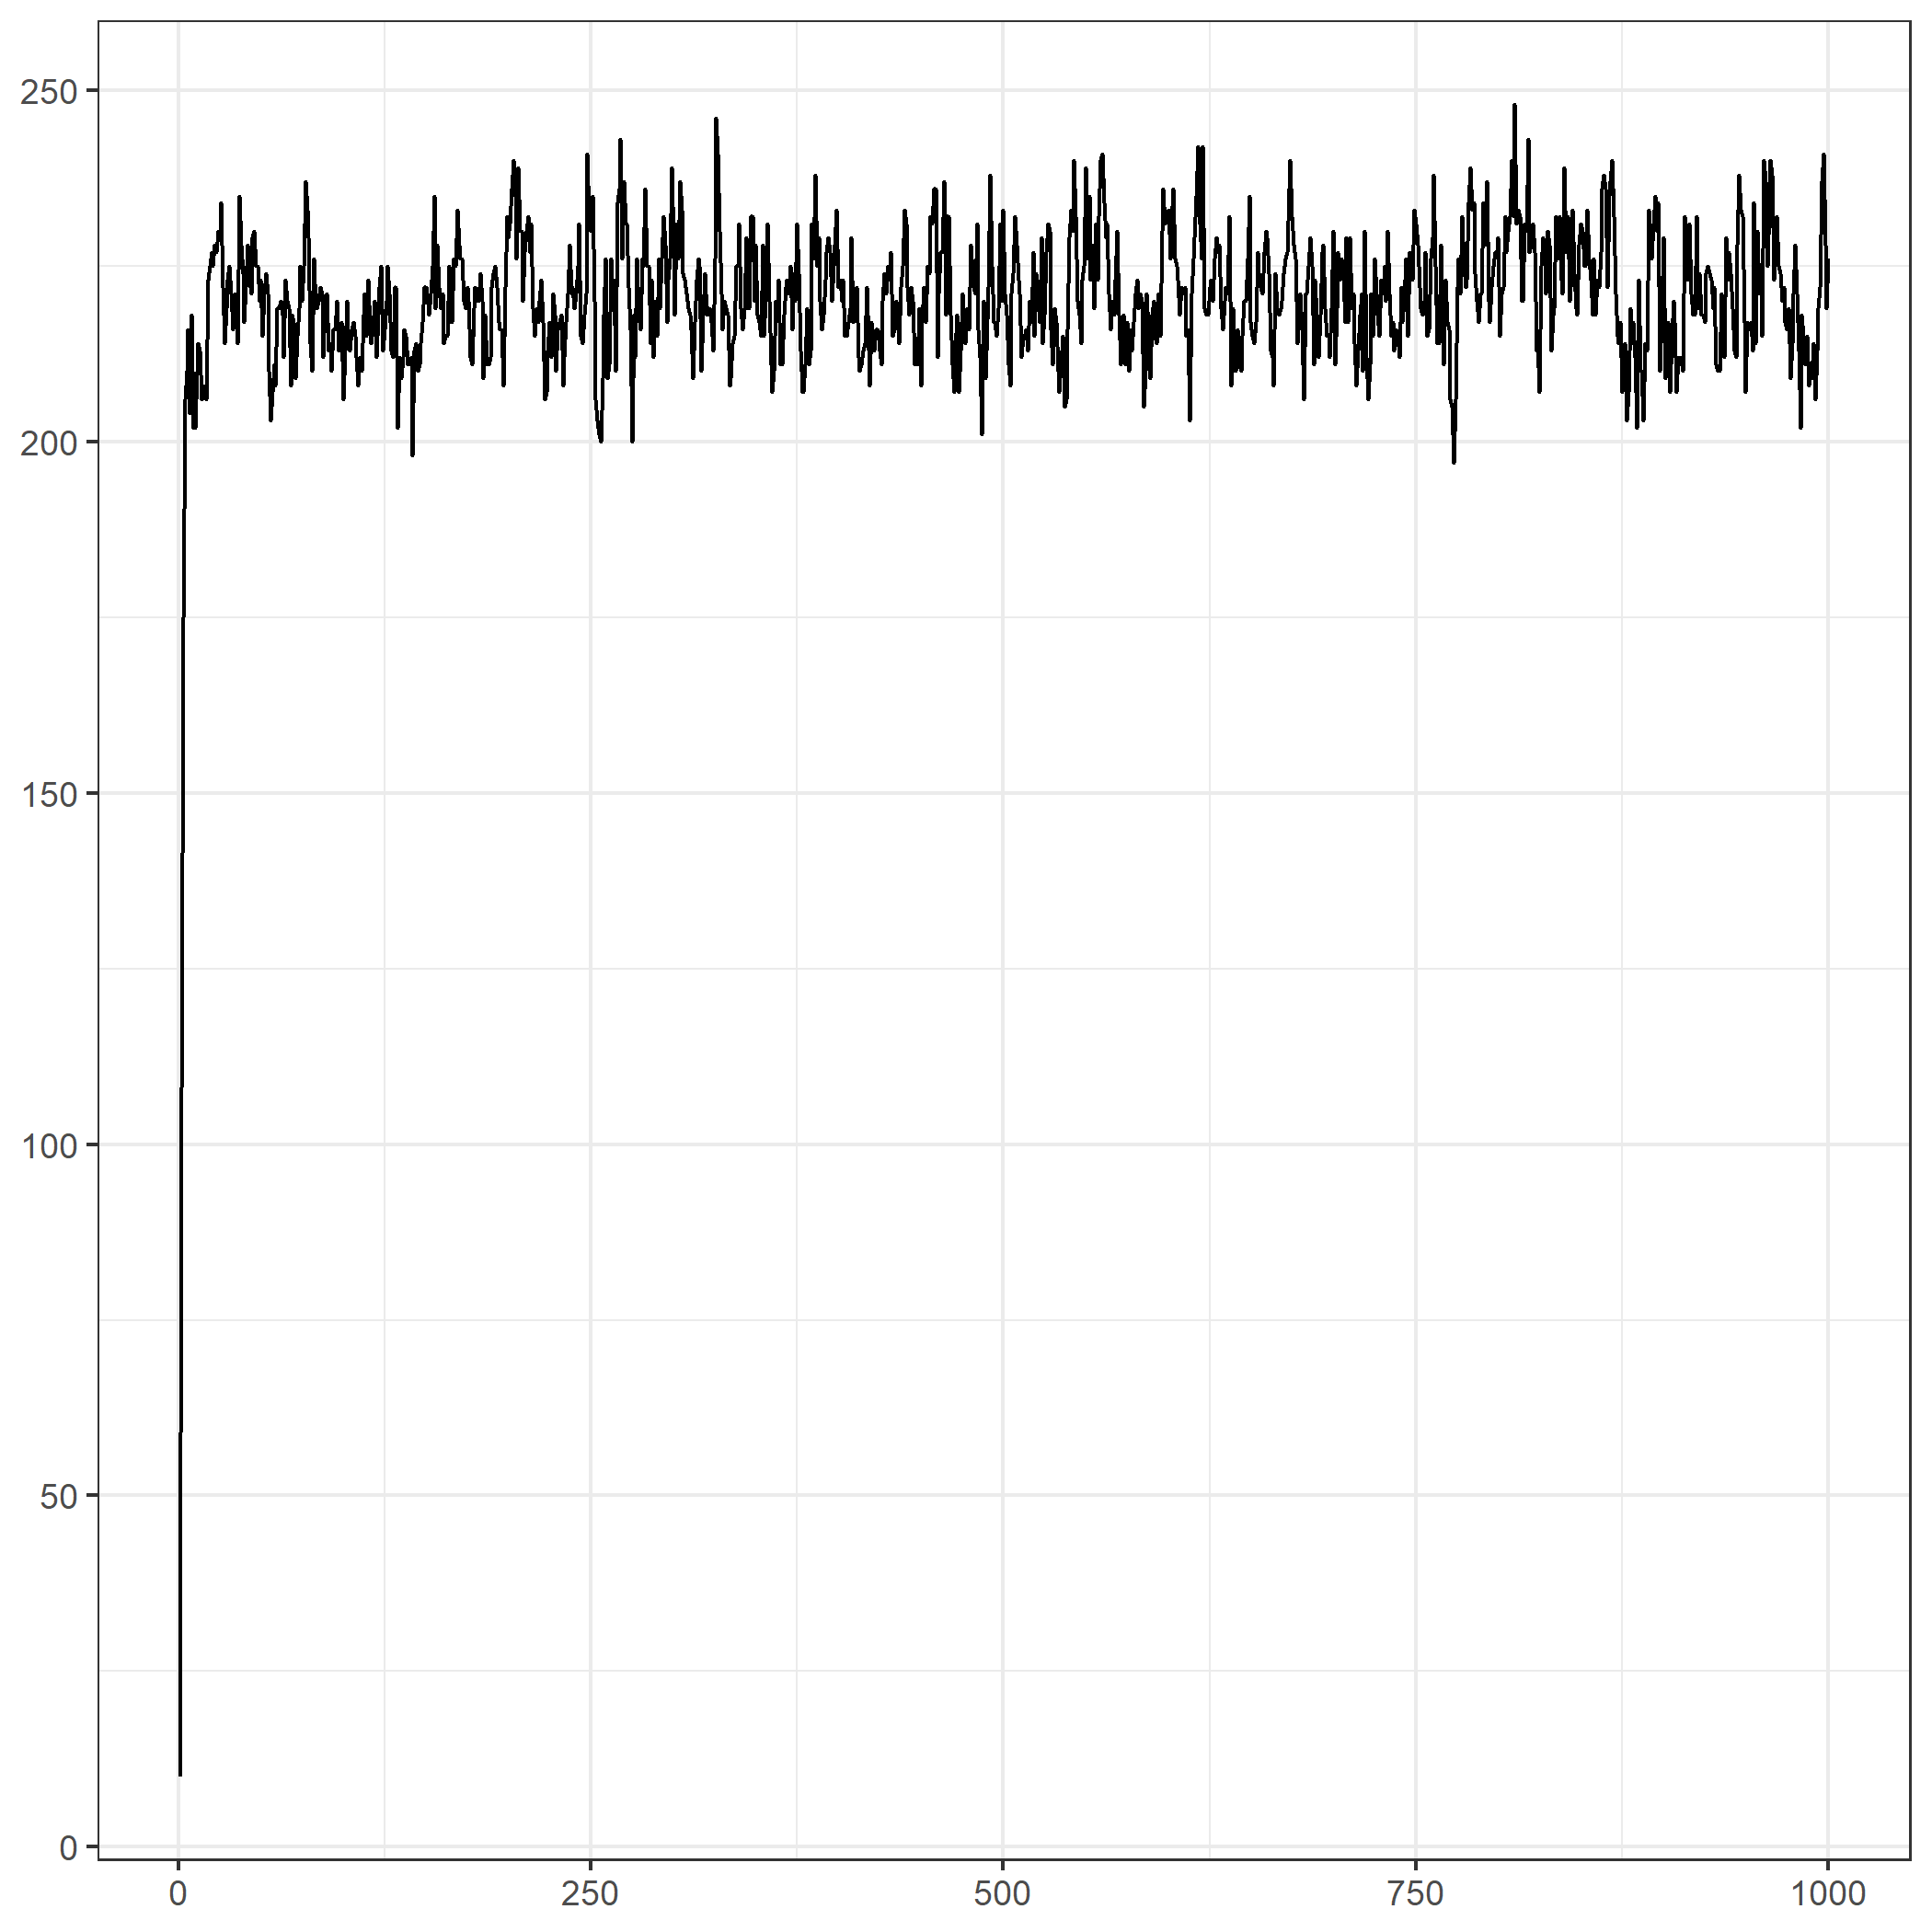
\includegraphics[width=0.6\textwidth]{../notes/figures/el_salvador/overlap_trace} 
			\caption{Traceplot for number of matches found across datasets in El Salvador case study}\label{fig:overlap_trace}
		\end{center}
	\end{figure}
	
	\begin{figure}[!h]
		\begin{center}
			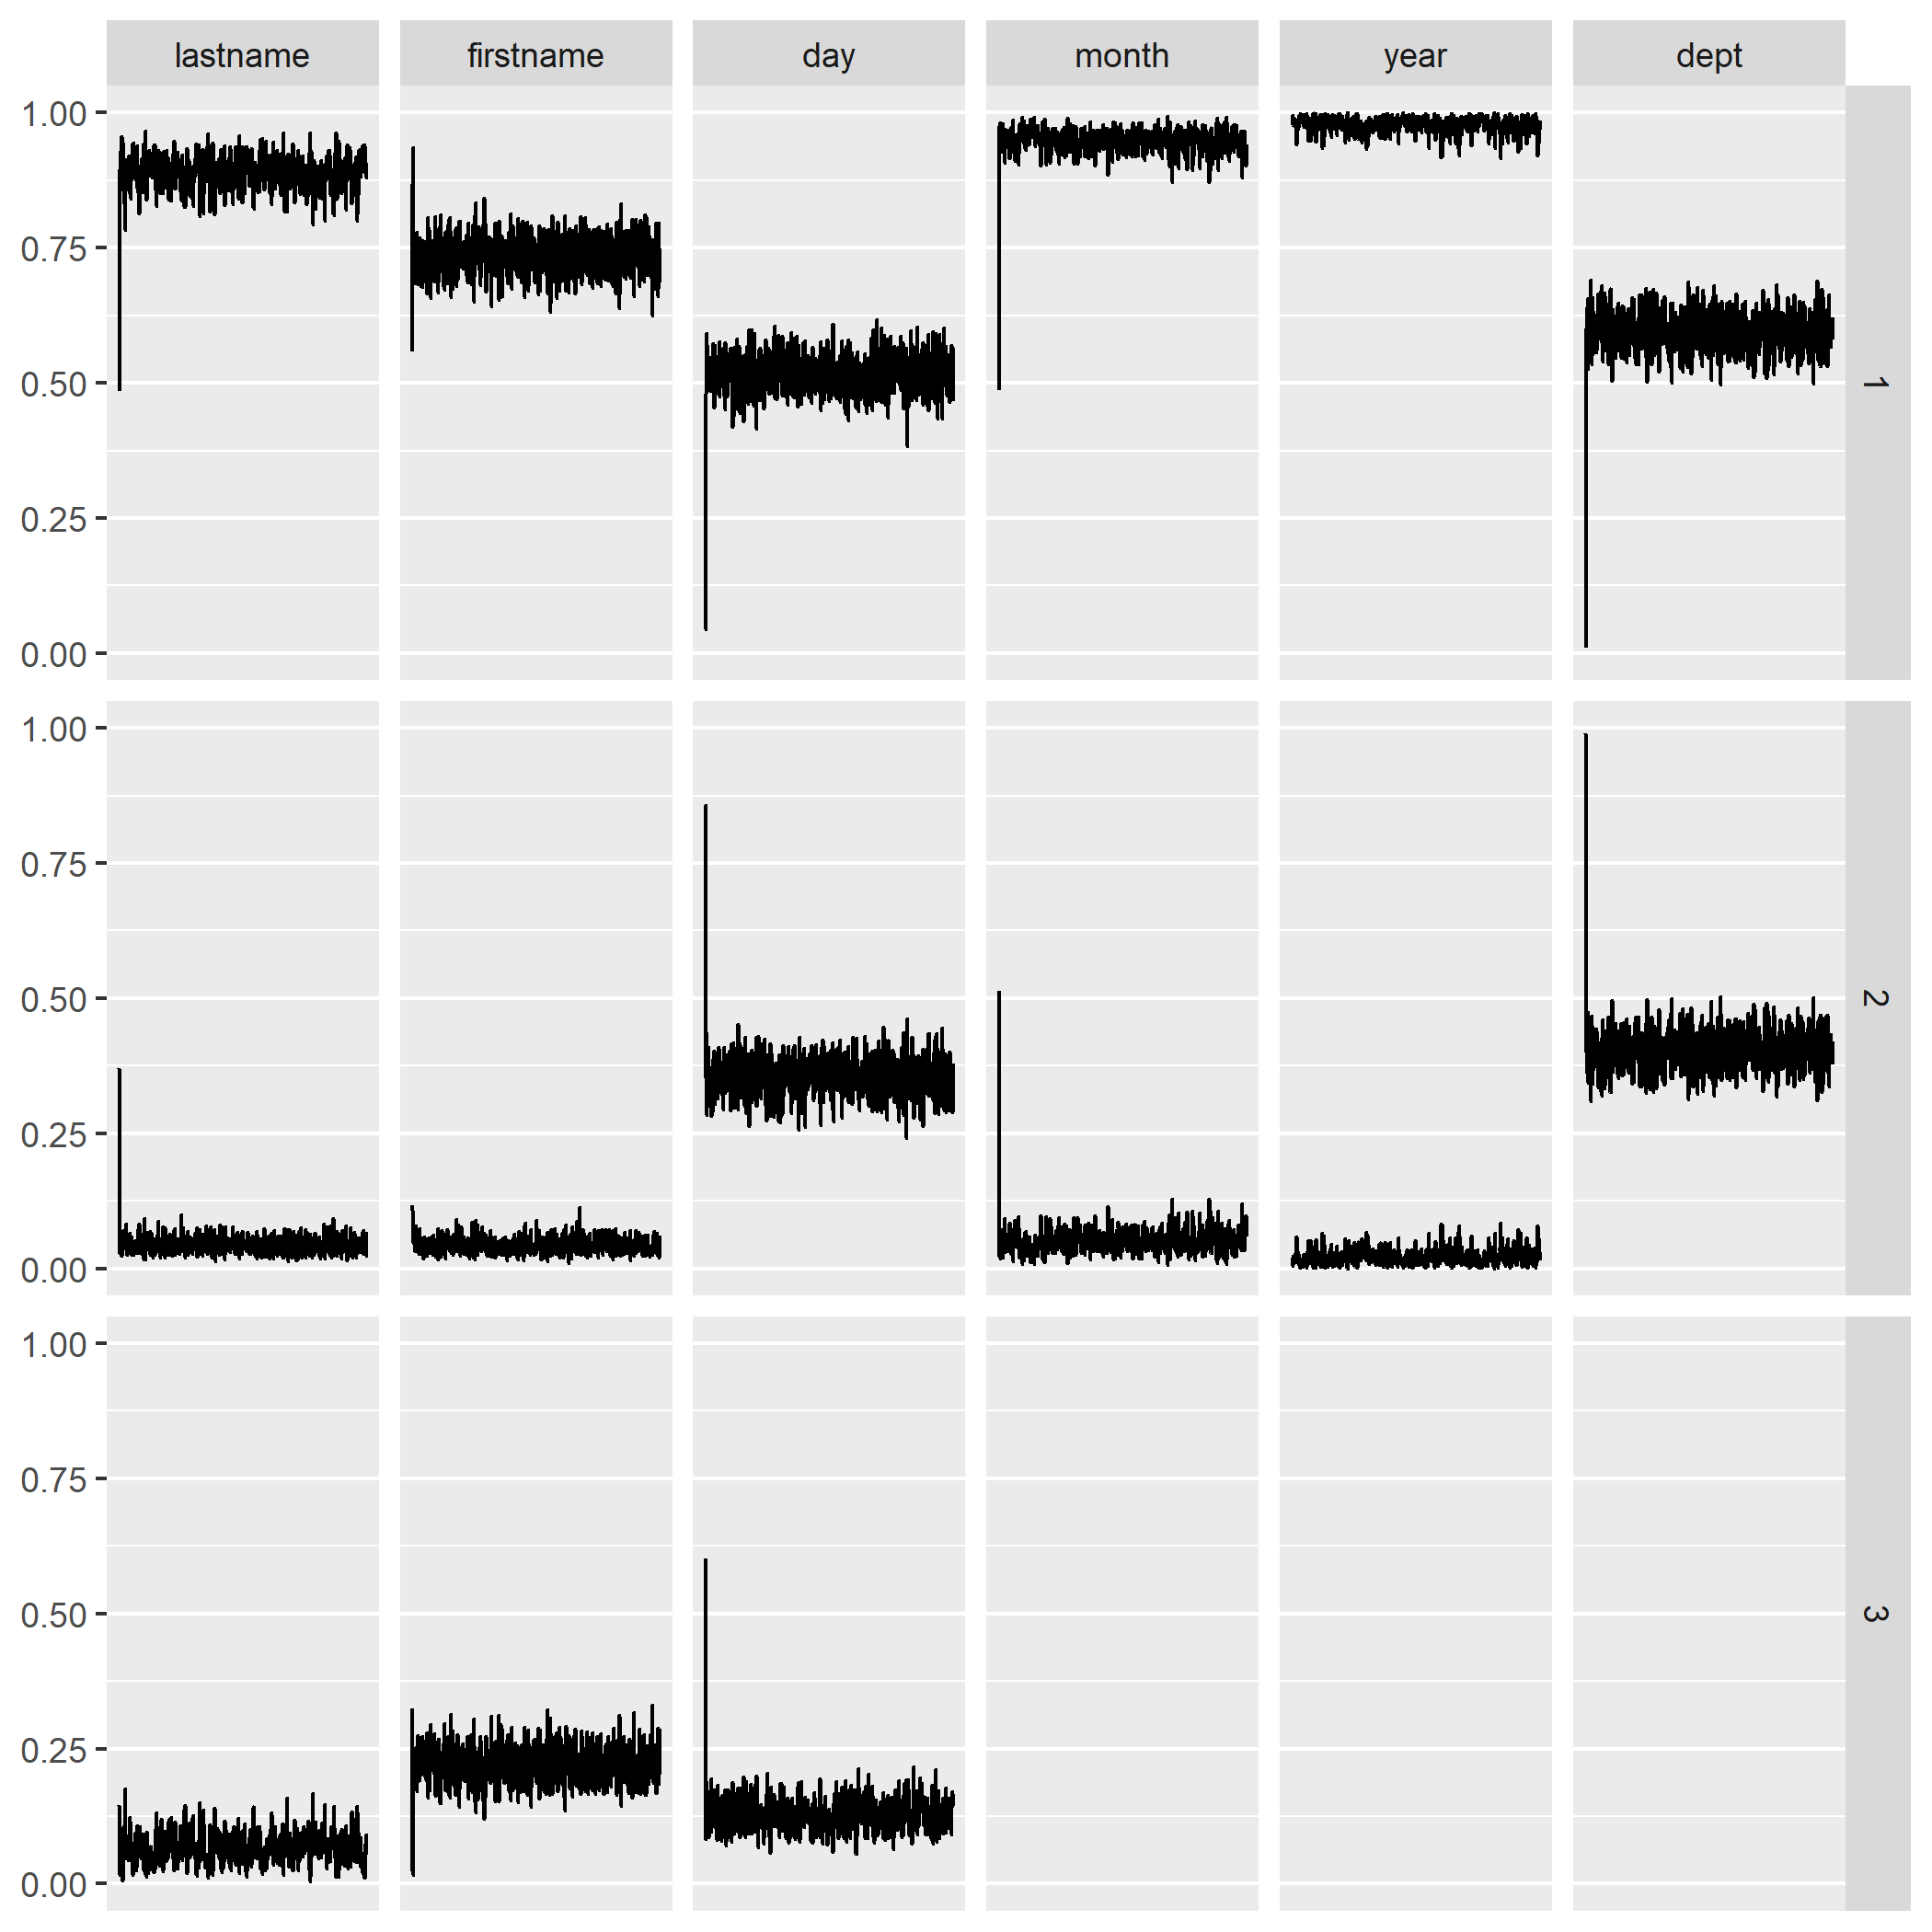
\includegraphics[width=0.6\textwidth]{../notes/figures/el_salvador/m_trace} 
			\caption{Traceplot for m parameter in El Salvador case study}\label{fig:m_trace}
		\end{center}
	\end{figure}
	
	\begin{figure}[!h]
		\begin{center}
			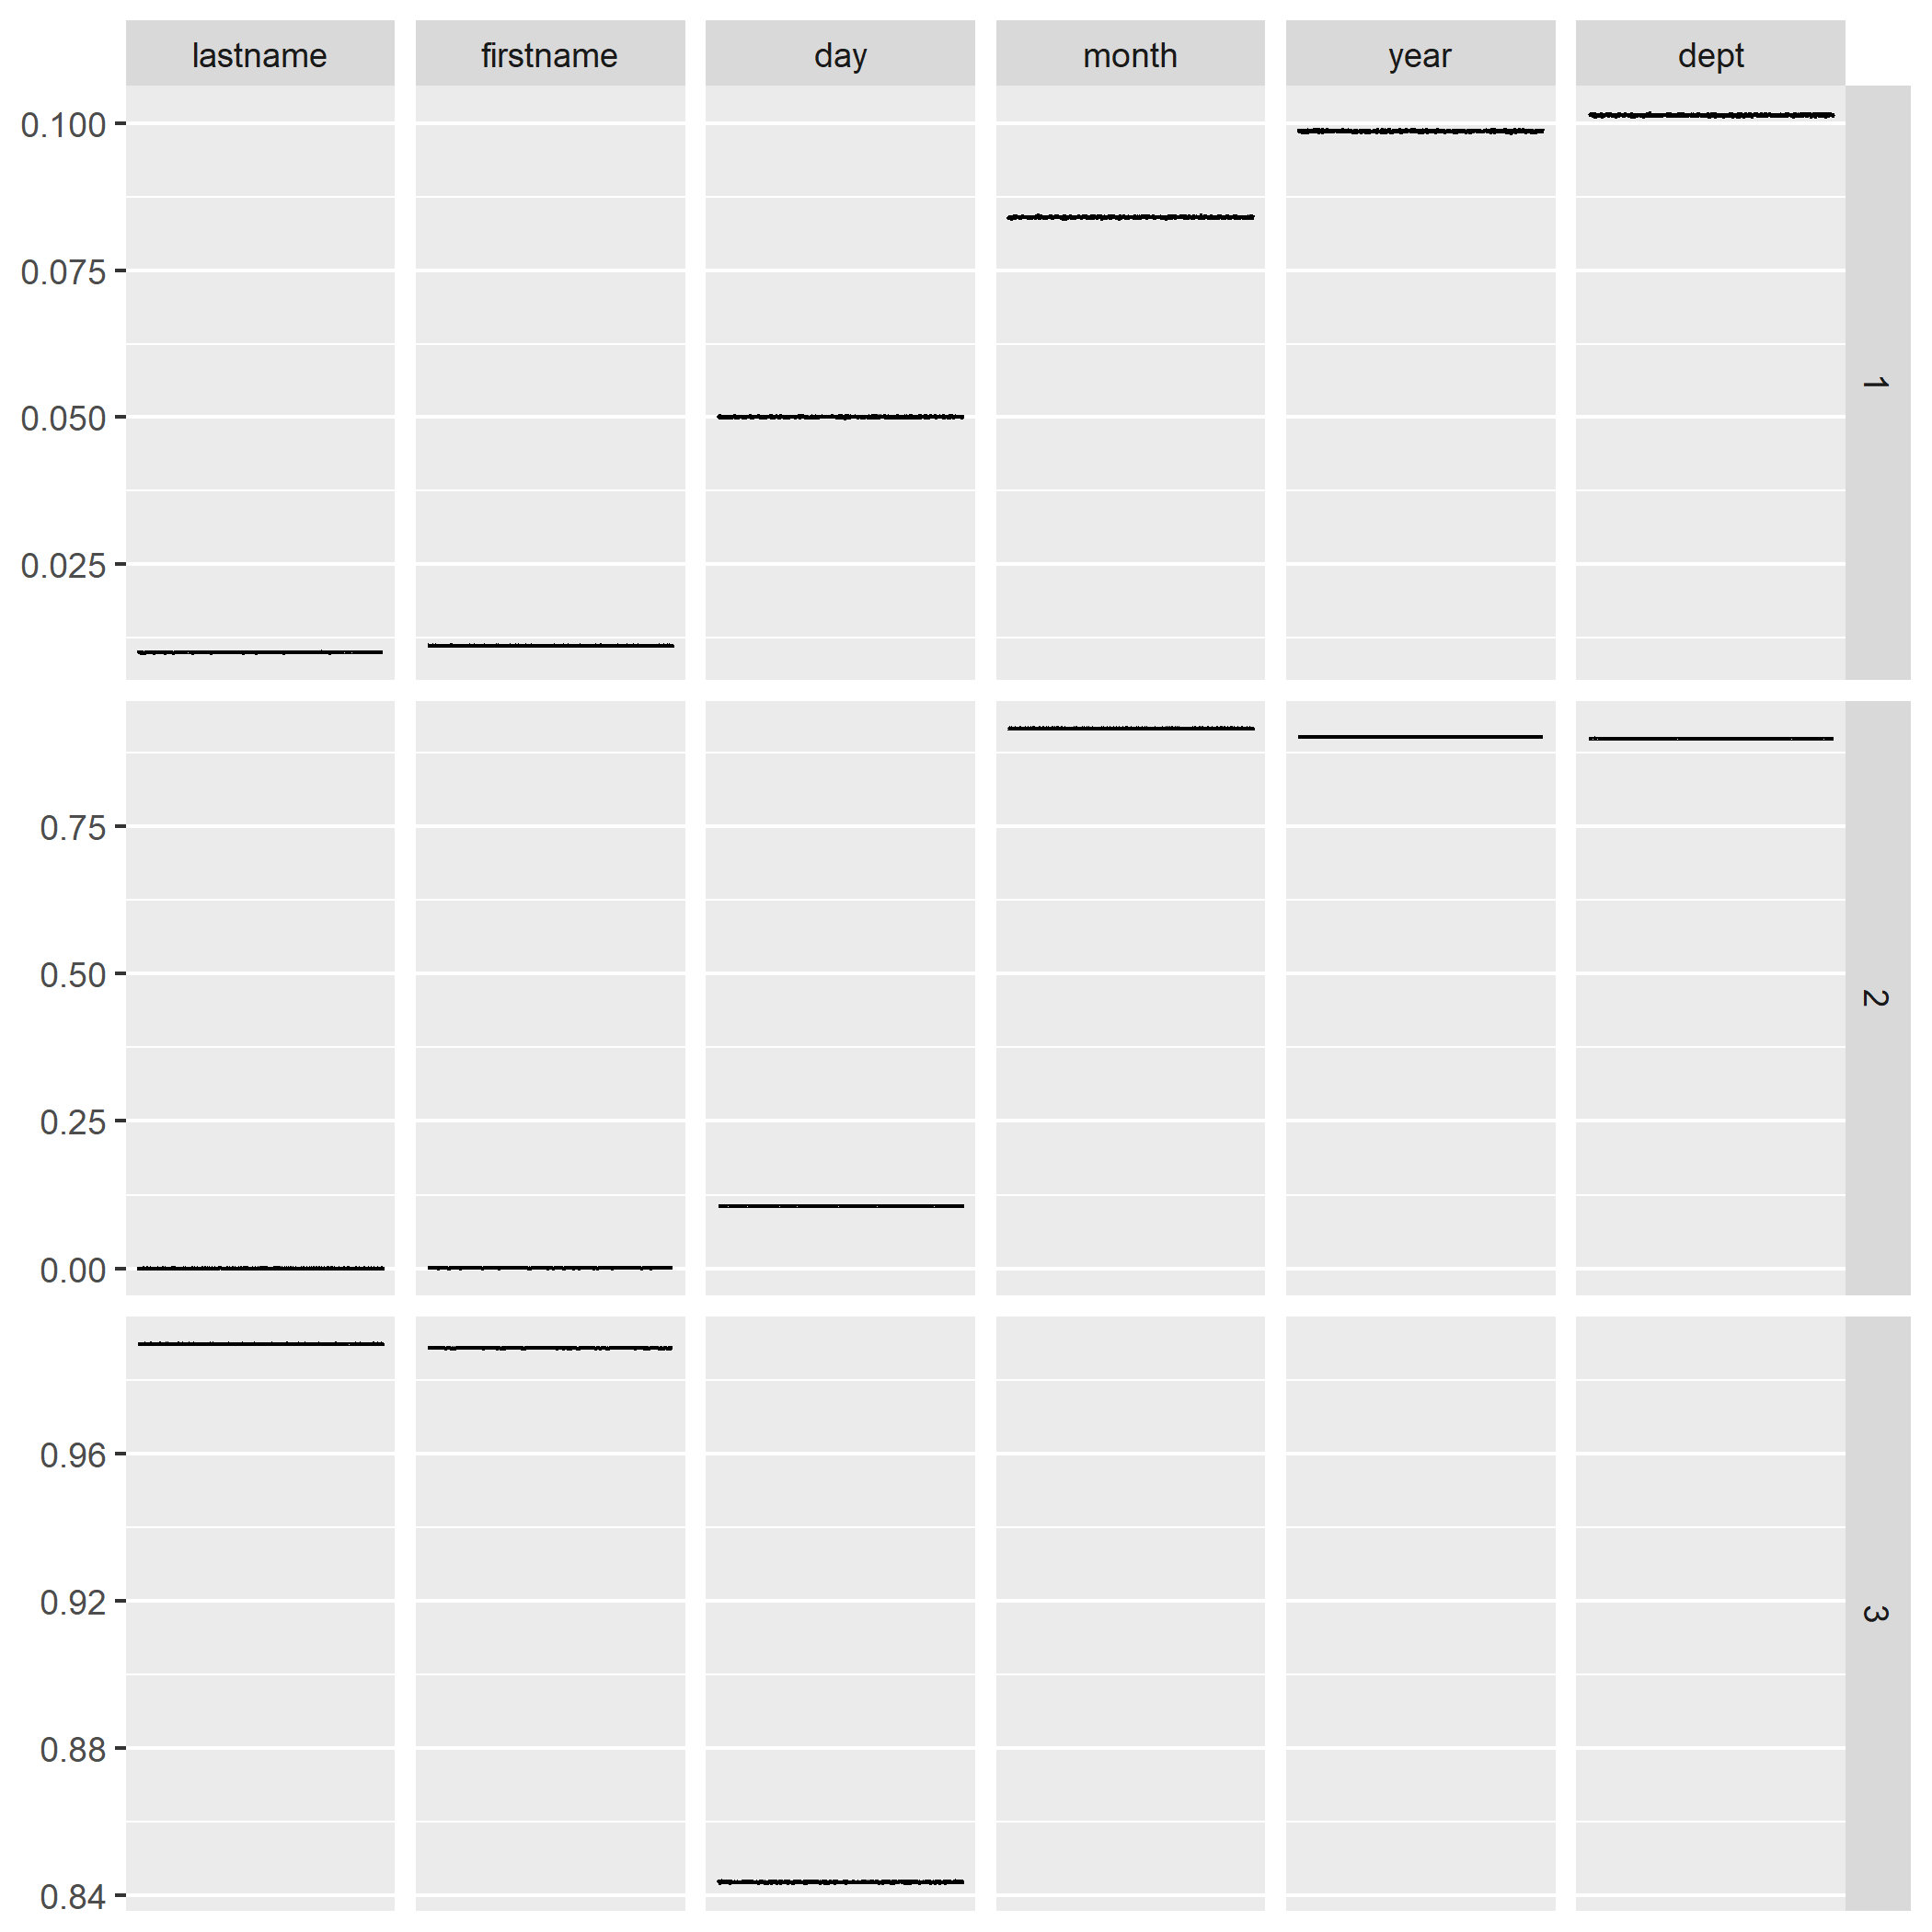
\includegraphics[width=0.6\textwidth]{../notes/figures/el_salvador/u_trace} 
			\caption{Traceplot for u parameter in El Salvador case study}\label{fig:u_trace}
		\end{center}
	\end{figure}
\end{document}
